% =====================================================================
%  Memoria del Trabajo Final de Máster
%  Plantilla propia que replica el aspecto del TFM modelo (UJI, 2025):
%  clase book, A4, babel inglés (memoria íntegramente en inglés americano), hyperref, IEEEtran.
% =====================================================================
\documentclass[a4paper,11pt,oneside]{book}

% --- Idioma y fuentes. Funciona con pdfLaTeX (por defecto en Overleaf) y con XeLaTeX/LuaLaTeX.
\usepackage{iftex}
\ifPDFTeX
  \usepackage[utf8]{inputenc}
  \usepackage[T1]{fontenc}
  \usepackage{lmodern}
  \usepackage[english]{babel}
\else
  \usepackage{fontspec}
  \setmainfont{Latin Modern Roman}[SmallCapsFont={Latin Modern Roman Caps}]
  \setsansfont{Latin Modern Sans}
  \setmonofont{Latin Modern Mono}
  \usepackage{polyglossia}
  \setmainlanguage{english}
\fi
\usepackage[a4paper,top=2.5cm,bottom=2.5cm,left=3cm,right=2.5cm]{geometry}
\usepackage{graphicx}
\usepackage{booktabs}
\usepackage{array}
\usepackage{longtable}
\usepackage{multirow}
\usepackage{tabularx}
\usepackage{caption}
\usepackage{subcaption}
\usepackage{amsmath,amssymb}
\usepackage{enumitem}
\usepackage{xcolor}
\usepackage{microtype}
\usepackage{csquotes}
\usepackage{setspace}
\usepackage{float}
\usepackage{rotating}
\usepackage{tikz}
\usetikzlibrary{arrows.meta,positioning,shapes.geometric,calc,fit,backgrounds}
\usepackage{pgfplots}
\pgfplotsset{compat=1.18}
\usepackage[hidelinks,pdfusetitle]{hyperref}
\usepackage{url}
\usepackage{emptypage}
\usepackage{etoolbox}
% IEEEtran.bst escribe «et al.» en cursiva; la norma de formato lo exige en redonda
\AtBeginEnvironment{thebibliography}{\renewcommand{\emph}[1]{\ifstrequal{#1}{et~al.}{et~al.}{\textit{#1}}}}

\graphicspath{{figuras/}}
\captionsetup{font=small,labelfont=bf}
\setlength{\parskip}{6pt}
\onehalfspacing
\setlist{nosep}
\newcolumntype{L}[1]{>{\raggedright\arraybackslash}p{#1}}
\newcolumntype{C}[1]{>{\centering\arraybackslash}p{#1}}
\newcommand{\code}[1]{\texttt{#1}}
\setlength{\emergencystretch}{2em}

% ---------- datos de la portada ----------
\newcommand{\tfmTitulo}{Evaluating Algorithms for Predictive Process Monitoring in Adult Inpatient Care Processes}
\newcommand{\tfmAutorNombre}{Miguel}
\newcommand{\tfmAutorApellidos}{Rebolledo Romero}
\newcommand{\tfmTutorA}{Reyes \textsc{Grangel Seguer}}
\newcommand{\tfmTutorB}{Juan Carlos \textsc{Amengual Argudo}}
\newcommand{\tfmMaster}{University Master's Degree in Intelligent Systems}
\newcommand{\tfmFecha}{October 27, 2026}
\newcommand{\tfmCurso}{2025/2026}
\newcommand{\HRule}{\rule{\linewidth}{0.5mm}}

\begin{document}

% =====================================================================
\frontmatter
\pagestyle{empty}

% ---------- Portada (plantilla UJI / VALGRAI) ----------
\begin{titlepage}
\begin{center}

% Logotipos

\includegraphics[width=0.18\textwidth]{logoUJI2.jpg}~\\[2cm]

\textsc{\LARGE \tfmMaster}\\[1.5cm]

\textsc{\LARGE Master Thesis}\\[1.5cm]
%%%%%%\textsc{\LARGE Provisional Version}\\[1.5cm]

% Título
\HRule \\[0.4cm]
{ \huge \bfseries \tfmTitulo \\[0.4cm] }
\HRule \\[1.5cm]

% Autor y supervisores
\begin{minipage}{0.48\textwidth}
\begin{flushleft} \large
\emph{Author:}\\
\tfmAutorNombre\ \textsc{\tfmAutorApellidos}
\end{flushleft}
\end{minipage}
\begin{minipage}{0.48\textwidth}
\begin{flushright} \large
\emph{Supervisors:} \\
\tfmTutorA \\
\tfmTutorB
\end{flushright}
\end{minipage}

\vfill

% Pie de la portada
{\large Date of presentation: \tfmFecha\\
Academic year \tfmCurso}

\end{center}
\end{titlepage}

% ---------- Dedicatoria ----------
\cleardoublepage
\vspace*{\fill}
\begin{flushright}
\itshape
[Dedication]
\end{flushright}
\vspace*{\fill}

% ---------- Agradecimientos ----------
\cleardoublepage
\chapter*{Acknowledgments}
I would like to express my gratitude to my supervisors, Reyes Grangel Seguer and Juan Carlos Amengual Argudo, for their guidance and dedication throughout this work, and for the methodological decisions that have given it its final shape. I thank the \emph{Hospital Universitari de La Plana} for providing the data on which the study has been built. I also thank the two research groups of Universitat Jaume I that work with them, the \emph{Grupo de Investigaci\'on en Aprendizaje Autom\'atico para Entornos Inteligentes} (GIANT) and the \emph{Grupo de Investigaci\'on en Enfermer\'ia} (GIENF), for the access to the database and their support during its analysis. Finally, I thank my family for their patience during the months of work.

% ---------- Resumen ----------
\cleardoublepage
\chapter*{Abstract}
The research work presented in this report aims to apply Predictive Process Monitoring (PPM) techniques to adult inpatient data, with the objective of experimentally comparing several prediction algorithms on a real care process. As a prior step to the predictive work, classic Process Mining (PM) techniques were applied to the \code{ftr\_cige\_v01} database. An event log of the elective surgical admission care process was built and the process was modeled in Business Process Model and Notation (BPMN). The event log was analyzed with four PM tools (ProM, Disco, Celonis and PM4Py) and validated, together with the model, by means of process discovery and conformance checking. The event log is built around the observable precursors of Failure To Rescue (FTR): ICU admission, prolonged length of stay and death.

On that event log, five prediction algorithms were evaluated, Decision Tree (DT), Random Forest (RF), Extreme Gradient Boosting (XGBoost), Long Short-Term Memory (LSTM) and Transformer, for three prediction types: next-activity prediction, the prediction of ICU admission without planning information and the prediction of prolonged length of stay. The results show that the next activity is predicted with an accuracy clearly above that of a trivial predictor, and that both ICU admission and prolonged length of stay can be anticipated with high discriminative ability. Sequence models outperform the classical ensemble by a small margin, while RF proves to be the most robust and best calibrated model, which agrees with what the process entropy predicts by placing the event log in the medium band. As future lines, hyperparameter tuning, calibration and explainability of the models are pointed out, as well as the extension of the studied population to address the scarcest clinical outcomes.

\section*{Keywords}
Process Mining, Predictive Process Monitoring, Event Log, Failure To Rescue, Inpatient Care, Machine Learning.

% ---------- Índices ----------
\cleardoublepage
\pagestyle{plain}
\tableofcontents
\cleardoublepage
\listoffigures
\cleardoublepage
\listoftables
\cleardoublepage
\chapter*{List of Acronyms}
\begin{longtable}{@{}p{3.4cm}p{11.2cm}@{}}
AUC-PR & Area under the precision--recall curve \\
AUC-ROC & Area under the receiver operating characteristic curve \\
BiLSTM & Bidirectional Long Short-Term Memory \\
BPIC & Business Process Intelligence Challenge \\
BPM & Business Process Management \\
BPMN & Business Process Model and Notation \\
CNN & Convolutional Neural Network \\
CPU & Central processing unit \\
CSV & Comma-separated values \\
DAW-Transformer & Dynamic Attribute-Aware Transformer \\
DFG & Directly-follows graph \\
DL & Deep Learning \\
DT & Decision Tree \\
ECTS & European Credit Transfer and Accumulation System \\
FFN & Feed-forward network \\
FTR & Failure To Rescue \\
GIANT & \emph{Grupo de Investigaci\'on en Aprendizaje Autom\'atico para Entornos Inteligentes} \\
GIENF & \emph{Grupo de Investigaci\'on en Enfermer\'ia} \\
ICD-10 & International Classification of Diseases, 10th revision \\
ICU & Intensive care unit \\
iDHM & Interactive Data-aware Heuristics Miner \\
LSTM & Long Short-Term Memory \\
ML & Machine Learning \\
PM & Process Mining \\
PPM & Predictive Process Monitoring \\
ReLU & Rectified linear unit \\
RF & Random Forest \\
ROC & Receiver operating characteristic \\
SHAP & SHapley Additive exPlanations \\
TFM & \emph{Trabajo de Fin de M\'aster} (Master's Thesis) \\
UJI & Universitat Jaume I \\
XAI & Explainable Artificial Intelligence \\
XES & eXtensible Event Stream \\
XGBoost & Extreme Gradient Boosting \\
\end{longtable}

% =====================================================================
\mainmatter
\pagestyle{headings}

\chapter{Introduction}
\label{cap:introduccion}

This chapter introduces the work carried out. It explains the healthcare and technological context in which the research is framed and the motivation behind it, presents the objectives set out in the proposal and the scope that was defined, describes the technological framework employed, the methodology and the follow-up of the project, and ends with the structure of this report.

\section{Context and Motivation}
\label{sec:contexto}

During the care of an inpatient, data of very different nature are continuously recorded. Each admission generates an administrative record of entry and discharge and, throughout the stay, surgical interventions, inter-service consultations, transfers between units, nursing assessments, vital signs and laboratory results, among other data. Taken together, these data describe the \emph{care process} that each patient follows from admission to discharge. Although they are recorded for care and management purposes, they can be transformed into an \emph{event log}. That event log can then be analyzed with Process Mining (PM) techniques in order to understand how care flows actually unfold and to improve patient safety \cite{aalst2016}.

One of the challenges of the inpatient care process is the early identification of the adverse situations that lead to what the medical literature calls Failure To Rescue (FTR). FTR is the inability to prevent the deterioration of a patient once a complication has appeared \cite{silber1992}. It is a phenomenon that is still poorly characterized in the medical literature, particularly regarding the data that precede it in hospital information systems. It is therefore of interest to analyze the situations that may lead to an FTR from the data that the hospital already records, with the aim of anticipating them. These situations are the unplanned admission to the intensive care unit (ICU), the prolonged length of stay and the onset of postoperative complications. That is the clinical motivation of this work.

From a technical point of view, PM \cite{aalst2016} provides the appropriate framework to address the problem. It makes it possible to build an event log from hospital data, to discover the process that patients follow and to compare it with the expected process. Its predictive branch, Predictive Process Monitoring (PPM) \cite{difrancescomarino2022,teinemaa2019}, builds models capable of anticipating how a case that is still running will continue. PPM covers different prediction types, such as the next activity, the remaining time, risks or the final outcome of the case \cite{difrancescomarino2022}. It relies on Machine Learning (ML) algorithms ranging from decision trees and their ensembles to sequential neural networks. An open question in the field is which family of algorithms suits each process. Zare et al.\ \cite{zare2025} propose answering it before training any model by means of the \emph{process entropy}, and this work evaluates that proposal on a real care process.

The present work is part of a broader research project on the characterization of FTR in inpatients by means of ML and PM techniques. In that project, the \emph{Hospital Universitari de La Plana} collaborates with two research groups of Universitat Jaume I (UJI): the \emph{Grupo de Investigaci\'on en Aprendizaje Autom\'atico para Entornos Inteligentes} (GIANT) and the \emph{Grupo de Investigaci\'on en Enfermer\'ia} (GIENF). The \code{ftr\_cige\_v01} database comes from that project. It is hosted on a UJI server and contains, in anonymized form, the data of the adult patients hospitalized between March 2023 and April 2024. In addition to demographic data, the data included are diagnoses, surgical interventions, inter-service consultations, transfers between units, nursing assessments, vital signs and laboratory results. They are real, heterogeneous data with the limitations inherent to a clinical information system. This makes them a suitable case study to assess to what extent PPM techniques, usually developed and evaluated on public event logs, are applicable in a clinical setting.

\section{Objectives}
\label{sec:objetivos}

The main objective of this \emph{Trabajo de Fin de M\'aster} (TFM) is \textbf{to evaluate and compare different PPM algorithms applied to healthcare event logs of inpatients}. This general objective is broken down into the sub-objectives listed below, stated as they appear in the thesis proposal, with the acronyms normalized to those used in this report, and followed by a brief explanation of how each one was addressed.

\begin{enumerate}[leftmargin=*]
  \item \textbf{Transform the healthcare dataset into an event log suitable for Process Mining and Predictive Process Monitoring analysis.} An event log was built from the hospital database, with case identifiers, activities, timestamps and contextual attributes.
  \item \textbf{Analyze the structure and characteristics of the generated healthcare event log.} The event log was analyzed by means of process discovery techniques and conformance checking against a reference model.
  \item \textbf{Study the state of the art of Predictive Process Monitoring methods, including model-based and Machine Learning-based approaches.} The PPM literature was reviewed and the experimental framework best suited to the clinical problem was identified.
  \item \textbf{Select the most suitable algorithms to apply to the dataset.} Five algorithms representative of the ML families used in PPM were selected.
  \item \textbf{Implement and evaluate several predictive algorithms for outcome prediction in healthcare processes.} The algorithms were implemented and evaluated on the event log for three prediction types.
  \item \textbf{Compare different predictive approaches, including model-based and ML-based.} Both families were considered in the planning; after the literature analysis it was decided to focus the comparison on ML-based approaches, as explained in Chapter~\ref{cap:relatedwork}.
  \item \textbf{Evaluate predictive performance using metrics such as accuracy, precision, recall, F1-score and AUC-ROC.} The results were evaluated with these metrics (AUC-ROC is the area under the receiver operating characteristic curve) and with complementary ones suited to imbalanced classes.
  \item \textbf{Identify the most suitable predictive approaches for healthcare event logs related to Failure To Rescue scenarios.} The most suitable algorithms were identified and the results were contrasted with those predicted by the process entropy.
\end{enumerate}

\section{Scope}

The project database contains a large amount of data of different nature about each hospitalization episode. In a first iteration of the work it was decided to narrow the study to the adult inpatient care process, considering only the events of the process: admissions, interventions, consultations, transfers and discharges. Vital-sign readings, laboratory results and nursing assessments were discarded because, owing to their frequency and nature, they do not describe the flow of the process but the state of the patient. The complete process has four branches, defined by two attributes of the admission: the admission type (elective or urgent) and the process type (surgical or medical). In a second iteration, in view of the variability of the complete process, the study was narrowed to one of the four branches, the \textbf{elective surgical care process}, i.e., to the episodes whose admission type is elective (scheduled) and whose process is surgical. This process is modeled with a Business Process Model and Notation (BPMN) diagram designed for this work. Its event log is built solely from the hospitalization, consultations, surgical interventions and transfers tables.

Regarding prediction, the work focuses on three prediction types. The first is next-activity prediction, which is the reference prediction of the experimental approach followed and allows a direct comparison with the literature. The other two are outcome predictions and answer the clinical question of the project: the prediction of ICU admission without using the planning information recorded in the operating theater, and the prediction of prolonged length of stay. Two other clinical targets are also explored, unplanned ICU admission and postoperative complication. Because of the number of available cases or the nature of the label, they are presented as complementary analyses.

The five algorithms evaluated are run with a basic configuration, without hyperparameter search, so that the comparison is between model families rather than between tuning efforts. Tuning, calibration and explainability of the models are left as future work.

\section{Technological Framework}
\label{sec:marco}

The work was carried out with four PM tools, which are used in the analysis of the event log in Chapter~\ref{cap:implementacion}, and with a set of ML libraries. The event log was exported to the eXtensible Event Stream (XES) format for the first three tools.

\begin{itemize}[leftmargin=*]
  \item \textbf{ProM}\footnote{\url{https://promtools.org/}} \cite{verbeek2010} is the reference research environment in PM, with hundreds of plug-ins. ProM Lite 1.4 was used for the Interactive Data-aware Heuristics Miner (iDHM), the Inductive Miner and alignment-based replay.
  \item \textbf{Disco}\footnote{\url{https://fluxicon.com/disco/}} (Fluxicon) \cite{gunther2012}, version 4.2.6, is a desktop tool oriented to exploratory analysis, with frequency and performance process maps, filters and case and variant statistics.
  \item \textbf{Celonis}\footnote{\url{https://www.celonis.com/}} is a commercial cloud platform, used in its academic edition. It offers the Process Explorer and the Process Adherence Manager, which compares the event log with a reference BPMN model.
  \item \textbf{PM4Py}\footnote{\url{https://processintelligence.solutions/pm4py}} \cite{berti2019}, version 2.7, is an open-source Python library that implements event-log import from comma-separated values (CSV) and XES files, the directly-follows graph (DFG), the Inductive Miner, the Heuristics Miner, alignments and the conversion between BPMN, Petri nets and process trees. It was the main tool of the work because it is programmable and reproducible.
\end{itemize}

The source database was downloaded from a PostgreSQL server by means of PowerShell scripts and the work was done on its CSV export. The event log and the whole analysis were programmed in Python 3 with pandas and NumPy. The tree-based predictive models were implemented with scikit-learn and the Extreme Gradient Boosting (XGBoost) library, and the two neural networks with PyTorch, trained on a two-core central processing unit (CPU); the metrics come from scikit-learn and the figures from Matplotlib. The code, the results of the final run and the LaTeX sources of this report are available in a public GitHub repository\footnote{\url{https://github.com/mr7security/tfm-ppm-ftr}}; the event logs and the database are not published because they contain clinical data. The scripts were written as standalone Python files, with the support of an AI coding assistant (Claude Code, by Anthropic) for their development and debugging, and were executed from the Windows PowerShell console; the code is versioned with Git. The reference BPMN model was designed with Camunda Modeler. The intermediate reports were written in Markdown and converted to PDF, and this report was written in \LaTeX. The code and the results are organized with one script per experiment and one results folder per run; each script fixes the random seeds and writes its metric tables, figures and execution log, so that any figure or table in this report can be regenerated by running the corresponding script again on the event log.

\section{Methodology}
\label{sec:metodologia}

This section describes the academic context of the work and the initial planning and its deviations; the follow-up of the project by phases is described in Section~\ref{sec:seguimiento}.

\subsection{Context of the Work}

This TFM was carried out within the University Master's Degree in Intelligent Systems at UJI, as the compulsory course SIU043, with a workload of 14 European Credit Transfer and Accumulation System (ECTS) credits, which corresponds to 350 hours of student work. The work integrates knowledge from the courses Machine Learning (SJK003), Big Data Analytics (SJK006) and Process Mining (SJK013), and was developed under the supervision of two supervisors from the Department of Computer Languages and Systems.

\subsection{Project Planning}

Table~\ref{tab:planificacion} shows the schedule established in the thesis proposal, with the estimated hours for each task and its objective, up to a total of 348 hours; the remaining 2 hours of the 350 hours of the course correspond to the presentation of the work. The proposal structured the work in six phases. The first was the literature review and the definition of the predictive approach. The second, data preparation and event-log generation. The third, process modeling and feature engineering. The fourth, the implementation of the predictive models. The fifth, the experimental evaluation and the comparative analysis. The sixth, the interpretation of the results and the writing of this report.

\begin{table}[htbp]
\centering
\caption{Project planning with tasks and hours.}
\label{tab:planificacion}
\begin{tabular}{L{5.2cm}C{1.8cm}L{6.6cm}}
\toprule
Task & Planned hours & Objective \\
\midrule
Problem analysis & 15 & Understand the information domain \\
Study of process modeling & 10 & Propose and design a model of the care process \\
State-of-the-art study & 30 & Understand the literature related to the problem domain \\
Data preparation & 100 & Search, interpret, clean and format the information to apply PM \\
Process discovery & 10 & Apply discovery techniques to obtain the real model of the care process \\
Implementation of the predictive models & 120 & Program and test the predictive models on the case study \\
Analysis of results & 15 & Compare the results obtained \\
Supervision & 20 & Supervise the research work \\
Writing of technical reports & 28 & Document the work carried out and the skills acquired \\
\midrule
\textbf{TOTAL} & \textbf{348} & \\
\bottomrule
\end{tabular}
\end{table}

The plan was fulfilled in its entirety in terms of the objectives achieved, but it was necessary to redistribute the time among tasks, since some of them required more hours than initially estimated. Data preparation took longer than planned because the event log was built three times. A first version covering the complete hospital process was discarded when the scope was defined. A second version was built on the elective surgical admission process. A third version incorporated the postoperative destination as an activity in its own right, a decision that emerged from the discovery analysis. Process discovery also exceeded the ten hours estimated, since it was carried out with four tools and with conformance checking against two versions of the reference model. By contrast, the implementation of the predictive models was less costly than planned. Once the pipeline had been fixed in a preliminary test, the complete experiments ran in less than ten minutes of CPU time, and the time was devoted to the analysis of the results and to the writing of intermediate reports. Had all the objectives of the proposal been kept, with the complete hospital process and both families of predictive approaches, the time would clearly have exceeded the allocation.

\section{Project Follow-Up}
\label{sec:seguimiento}

The development followed a sequential and iterative approach. Each phase produced a technical report that was reviewed with the supervisors and conditioned the next one. This way of working made it possible to take two decisions that proved decisive, the definition of the scope and the incorporation of the postoperative destination into the event log, without redoing the previous work.

\subsection{Research Phase and Context Analysis}

This phase included the problem analysis, the state-of-the-art study and the study of process modeling. The literature analysis, reported in Chapter~\ref{cap:background} and~\ref{cap:relatedwork}, covered PM in healthcare, PPM in its different prediction types, and the evaluation benchmarks of the field. From that analysis it was concluded that the Entropy-Driven Next Activity Prediction Approach of Zare et al.\ \cite{zare2025} was the one that best fitted the clinical problem to be solved, for three reasons. It explicitly compares interpretable models with deep models, which is the comparison of interest in a clinical setting. It proposes a criterion prior to training, the process entropy, which can be applied to any event log. Moreover, one of its evaluation event logs comes from healthcare, which makes it possible to place the event log of this work on its scale. The structure of the \code{ftr\_cige\_v01} database, with its 20 tables and its catalogs, was also studied, and a first BPMN model of the care process was designed.

\subsection{Data Preparation and Event-Log Construction}

This was the central phase of the project. The database was downloaded from the UJI server by means of export scripts, its tables were exported to CSV and the event log was built in three successive versions. The first version covered the complete hospital process, with one event per clinical act, including vital-sign readings, laboratory tests and nursing assessments. It served for a first exploration with the discovery tools, but proved intractable for a dedicated reference model. The second version, after the definition of the scope, covered only the elective surgical admission, built from four tables and aligned with a BPMN model designed for this work. On this version a preliminary PPM test was run that fixed the experimental pipeline. The third version incorporated the postoperative destination planned at the exit of the operating theater as an activity in its own right, after observing in the discovery that this decision almost completely explains the planned ICU admissions. It is the final version, described in Chapter~\ref{cap:datos}.

In each version the data were checked for null values, duplicates and out-of-range dates, formats and encodings were unified, the relevant variables were selected and the warnings about possible information leakage were documented.

\subsection{Process Discovery and Conformance Checking}

On each version of the event log, discovery techniques (DFG, Inductive Miner and Heuristics Miner) were applied with ProM, Disco, Celonis and PM4Py, and conformance checking against the reference BPMN model with PM4Py and Celonis. The use of four tools served a twofold purpose. On the one hand, to validate that the event log is interpreted identically in all of them. On the other, to contrast the discovery algorithms with independent implementations. From this phase came the finding that conditions the experimental design, namely that the postoperative destination ICU implies ICU admission in 100\% of the cases.

\subsection{Design and Implementation of the Predictive Models}

The experimental design was fixed incrementally. A preliminary test on the second version of the event log established the prefixes, the two encodings, the temporal split and the basic configuration of the five prediction algorithms. On the third version, two sources of information leakage were identified and handled. The first is the planned postoperative destination recorded in the operating theater, which reveals the ICU admission: it gave rise to the variants of ICU-admission prediction, in which that information is hidden (A), kept (B) or made legitimate by restricting the population (C). The second is the number of coded diagnoses (\code{n\_diag}), which is assigned at discharge and grows with the complications: it was excluded from the models. Then prolonged length of stay and postoperative complication were added as targets. Finally, the three prediction types of the work were consolidated into a single reproducible run. Table~\ref{tab:cronologia} summarizes the milestones of this phase and the decision taken at each one.

\begin{table}[htbp]
\centering
\caption{Milestones of the predictive phase and the decision taken at each one.}
\label{tab:cronologia}
\small
\begin{tabular}{L{1.6cm}L{4.6cm}L{7.2cm}}
\toprule
Date & Milestone & Decision or finding \\
\midrule
Sep 17 & Scope narrowed with the supervisors & Only the elective surgical admission, with a BPMN model designed for this work and four tables of the database. Second version of the event log. \\
Sep 19 & Preliminary PPM test on the second version & Pipeline fixed: prefixes, two encodings, temporal split and five algorithms. Discriminative ability of 0.85--0.88 for ICU admission. \\
Sep 28 & Third version of the event log & The postoperative destination becomes an activity (\code{DESTINO\_*}). Discovery with four tools shows that \code{DESTINO\_UCI} always precedes \code{INGRESO\_UCI}. \\
Sep 29 & Variants A, B and C of ICU admission & The destination is planning, not prediction; leakage through \code{n\_diag} detected; next-activity prediction (F) added. \\
Oct 2 & Targets D and E; final run & Postoperative complication (D) and prolonged length of stay (E) added. Scope fixed: Predictions~1 (F), 2 (A) and 3 (E) in a single reproducible run. \\
\bottomrule
\end{tabular}
\end{table}

\subsection{Evaluation and Analysis}

The evaluation was iterative. Each experiment was documented in a report with its metric tables, curves and interpretation, which was discussed before deciding the next step. Special attention was paid to interpreting why a model performs as it does, i.e., which variables it uses, what happens when the prefix is lengthened and where information leakage may occur, and not only to comparing figures. That interpretation is what made it possible to identify that part of the apparent performance came from planning information and not from predictive ability.

\subsection{Future Work}

Throughout the project, the avenues that could not be addressed without deviating from the objectives were noted. Four of them stand out. Hyperparameter tuning and the calibration of the deep models would improve performance, but would not change the nature of the comparison. Explainability through SHapley Additive exPlanations (SHAP) values would make it possible to contrast with clinical judgment which variables support each prediction. An intermediate target of `unplanned complication', which excludes the planned ICU admissions, would have more cases than unplanned ICU admission without the heterogeneity of postoperative complication. Finally, the extension of the population to all surgical admissions, elective and urgent, would increase the number of cases of the scarcest outcomes. They are collected in Chapter~\ref{cap:conclusiones}.

\section{Structure of the Report}

The report is organized into six chapters.

\textbf{Chapter~\ref{cap:introduccion}}, Introduction, presents the context, the motivation, the objectives, the scope and the technological framework of the work, together with the methodology followed and the follow-up of the project by phases.

\textbf{Chapter~\ref{cap:background}}, Background, reviews the foundations on which the study rests: the clinical data of inpatients and the concept of FTR, PM, PPM and the ML algorithms compared.

\textbf{Chapter~\ref{cap:relatedwork}}, Related Work, reviews previous work on PPM and its application to healthcare processes, and presents in detail the Entropy-Driven Next Activity Prediction Approach of Zare et al.\ \cite{zare2025}, which this work adopts.

\textbf{Chapter~\ref{cap:datos}}, Data and Event Log, presents the source database, the reference BPMN model of the elective surgical admission process, the construction of its event log, its activities, attributes and candidate labels, the warnings about information leakage and the process entropy that condition the experimental design.

\textbf{Chapter~\ref{cap:implementacion}}, Implementation, covers process discovery and conformance checking with the four tools, the PPM experimental design, the results of the three prediction types (next activity, ICU admission and prolonged length of stay), the complementary analyses and the comparison with the protocol of Zare et al.\ \cite{zare2025}.

\textbf{Chapter~\ref{cap:conclusiones}}, Conclusions, summarizes the findings, contrasts them with the objectives and proposes lines of future work.

\chapter{Background}
\label{cap:background}

This chapter presents the foundations needed to put the project in context. First, the clinical data generated during the hospitalization of adult patients and the concept of FTR are described. Then PM and the concept of event log are introduced. After that, PPM is described, together with its prediction types and the usual way of evaluating it. The chapter ends with a description of the five ML algorithms compared in this work.

\section{Clinical Data of Inpatients and Failure To Rescue}
\label{sec:datos_clinicos}

During the hospitalization of an adult patient, the hospital information system records the episode from admission to discharge. Associated with the episode are the administrative data (admission and discharge dates, admission type, responsible service, discharge reason), the demographic data of the patient, the admission diagnosis and the diagnostic coding at discharge according to the International Classification of Diseases (ICD-10), and the care acts that take place during the stay. These acts include surgical interventions, with their type, anesthesia and postoperative destination; inter-service consultations; transfers between units, in particular to the ICU; nursing assessments; vital-sign readings; and laboratory results.

In the nursing field, the assessment of the inpatient relies on standardized indices that measure fall risk, functional capacity, pressure injury risk and comorbidity. The VALENF instrument \cite{lunaaleixos2022}, developed and validated in adult hospitalization units, integrates that assessment into a single meta-instrument. It is one of the sources of the nursing assessments recorded in the project database.

The term FTR was coined by Silber et al.\ \cite{silber1992} to describe the death of a patient after a complication that, had it been detected and treated in time, might not have been fatal. Unlike the raw complication rate, which depends mainly on the patient's risk, FTR reflects the hospital's ability to recognize deterioration and respond to it, and it has been proposed as an indicator of quality of care \cite{ghaferi2009}. However, FTR is not well characterized in the medical literature: there is no consensus on which complications to consider, on the time horizon or on the precursors that announce it. In hospital information systems, those observable precursors are unplanned admission to the ICU, urgent consultations, prolonged length of stay and, ultimately, death. Analyzing the situations that may lead to an FTR from the data recorded during hospitalization is therefore a necessary first step toward characterizing it.

The care process studied in this work is the elective surgical admission. It takes place as follows. The patient is admitted to the hospital on a scheduled date to undergo a planned surgery. Before the surgery, the surgical team assesses the postsurgical risk. If the risk is high, an ICU bed is reserved for the patient. The patient then goes through the operating theater. At the end of the surgery, the patient leaves the theater with a planned postoperative destination: the ward, the ICU, the post-anesthesia care unit or another unit. During the stay, the clinical team may request consultations to other specialists. If a complication arises, the patient may be transferred to the ICU or to another hospital. Finally, the patient is discharged. In this process, FTR manifests itself as the difference between what was planned and what happened: the patient whose planned destination was the ward and who ends up in the ICU, or whose stay is prolonged well beyond what was expected. That distinction between \emph{planning} and \emph{evolution} is central to the experimental design of Chapter~\ref{cap:implementacion}. The reference model of this process, designed for this work, is presented in Section~\ref{sec:modelo}.

\section{Process Mining}
\label{sec:pm}

PM is the discipline that connects data science with Business Process Management (BPM). From the records left by information systems, it extracts knowledge about how processes are actually executed \cite{aalst2016}. Its starting point is the event log, a collection of events each of which belongs to a case (an instance of the process), corresponds to an activity and carries a timestamp. Events may also carry additional attributes, such as the resource that executes them, the service or the result of a decision. The ordered sequence of the events of a case is called a trace, and the set of distinct traces that appear in the event log, variants.

Three types of analysis are distinguished on an event log \cite{aalst2016}.

\begin{itemize}[leftmargin=*]
  \item \textbf{Process discovery}. It consists of building a model of the process from the event log, without prior information. The most widely used algorithms are the Heuristics Miner, which builds a causal net from the frequency dependencies between activities and tolerates noise, and the Inductive Miner, which discovers process trees guaranteeing well-formed models \cite{leemans2014}. The DFG is the simplest representation, with one node per activity and one arc per pair of consecutive activities, annotated with its frequency.
  \item \textbf{Conformance checking}. It consists of comparing the event log with a reference model, either normative or discovered, in order to measure how far the observed behavior matches the expected one. The reference technique is \emph{alignments}, which search, for each trace, the most similar path in the model and quantify the deviations \cite{carmona2018}. From them are derived \emph{fitness}, which measures what fraction of the behavior in the event log the model explains, and \emph{precision}, which measures what fraction of the behavior of the model appears in the event log.
  \item \textbf{Enhancement}. It consists of enriching the model with performance, resource or decision information.
\end{itemize}

In healthcare, PM has been applied to emergency flows, oncology processes and patient trajectories, with the particularity that clinical processes are highly variable, poorly structured and strongly patient-dependent \cite{munoz2022}. That variability is the reason why the choice of the scope and of the granularity of the event log is a central decision of the work.

\section{Predictive Process Monitoring}
\label{sec:ppm}

PPM is the branch of PM that, from the historical event log, builds models capable of predicting how a case that is still running will continue \cite{difrancescomarino2022}. The unit of prediction is the prefix, formed by the first $k$ events of a trace. For each prefix, something about the future of the case is to be predicted. Di Francescomarino et al.\ \cite{difrancescomarino2018} classify PPM methods into three types according to what is predicted:

\begin{itemize}[leftmargin=*]
  \item \textbf{Outcome-based predictions}: predictions related to predefined categorical or boolean outcome values of the case, for example whether it will end in a deadline violation, in a complaint or, in this work, in an ICU admission \cite{teinemaa2019}.
  \item \textbf{Numeric value predictions}: predictions related to measures of interest taking numeric or continuous values, such as the remaining time until the end of the case \cite{aalst2011} or its cost.
  \item \textbf{Next event predictions}: predictions related to sequences of future activities and their data payloads, of which the prediction of the next activity is the simplest case \cite{tax2017}.
\end{itemize}

This classification is used in the rest of the report to name the three predictions carried out. Prediction~1 is a next event prediction (the next activity of the case). Predictions~2 and~3 are outcome-based predictions with a boolean outcome: whether the patient will be admitted to the ICU and whether the length of stay will be prolonged. No numeric value prediction is addressed.

PPM approaches are traditionally divided into two families \cite{difrancescomarino2018}. Model-based approaches rely on an explicit representation of the process, such as a transition system or a stochastic Petri net, annotated with statistics from the event log. ML-based approaches encode prefixes as feature vectors or as sequences and train a classifier or a neural network. Within this second family there are two ways of encoding a prefix \cite{teinemaa2019}. In aggregate encoding the prefix is summarized in a fixed-length vector with the count of each activity, the last activity, the elapsed times and the case attributes; it is the natural input of decision trees, ensembles and linear models. In sequence encoding the prefix is kept as a sequence of events, each represented by an embedding of its activity and by numerical features, padded up to a maximum length; it is the input of recurrent networks and Transformers.

The evaluation of a PPM model generally follows the protocol set by the benchmark of Teinemaa et al.\ \cite{teinemaa2019} for outcome prediction. Cases are split between training and test with a temporal split, so that the oldest cases train and the most recent ones evaluate. All prefixes of length $1 \ldots k_{\max}$ of each case are generated. Performance is measured with the area under the receiver operating characteristic (ROC) curve (AUC-ROC), which quantifies the ability of the model to rank positive cases above negative ones regardless of the decision threshold. The AUC-ROC is also reported per prefix length, because it is of interest to know how much the prediction improves as the case progresses. When the positive class is a minority, as happens with adverse clinical outcomes, the AUC-ROC can be high even if the model gets few positives right, because negatives dominate. For this reason it is complemented with the area under the precision--recall curve (AUC-PR), whose random baseline is the prevalence of the positive class \cite{saito2015}, and with the Brier score, which measures the calibration of the probabilities. For next-activity prediction, being a multiclass problem, accuracy and macro F1-score are used, against a baseline that predicts the most frequent transition.

\section{Machine Learning Algorithms Evaluated}

Five algorithms are compared, covering the two ML families usual in PPM: three tree-based models, which work on the aggregate encoding, and two sequential neural networks.

\paragraph{Decision Tree (DT).} A DT \cite{quinlan1986,breiman1984} recursively partitions the feature space by choosing at each node the variable and the threshold that best separate the classes. It is the most interpretable model, since the prediction is explained as a chain of conditions, but it tends to overfit and is unstable under small changes in the data. It is included as the interpretable reference model, as in Zare et al.\ \cite{zare2025}.

\paragraph{Random Forest (RF).} RF \cite{breiman2001} trains many trees on bootstrap samples of the training set, choosing at each node a random subset of variables, and averages their predictions. Averaging reduces the variance of the individual tree and yields well-calibrated probabilities, and it also provides a measure of variable importance. It is the reference ensemble in the benchmark of Teinemaa et al.

\paragraph{Extreme Gradient Boosting (XGBoost).} XGBoost \cite{chen2016} is an implementation of gradient boosting \cite{friedman2001} in which trees are built sequentially, each correcting the errors of the previous ensemble, with regularization and early stopping. It is usually the most accurate tabular model when its hyperparameters are tuned, but it is more sensitive to the configuration than RF.

\paragraph{Long Short-Term Memory (LSTM).} LSTM networks \cite{hochreiter1997} are recurrent networks with memory cells and gates that control what is remembered and what is forgotten, which allows them to capture dependencies along a sequence. Tax et al.\ \cite{tax2017} introduced them in PPM to predict the next activity and the remaining time, and since then they have been the reference Deep Learning (DL) model in the field.

\paragraph{Transformer.} The Transformer \cite{vaswani2017} replaces recurrence with a multi-head \emph{self-attention} mechanism that directly relates all the elements of the sequence to each other, with a positional encoding that preserves order. In PPM it has been applied both in its standard form (ProcessTransformer \cite{bukhsh2021}) and in variants that attend to each attribute separately, such as the Dynamic Attribute-Aware Transformer (DAW-Transformer) of Zare et al.\ \cite{zare2025}. In this work a standard Transformer encoder of reduced size is used, in accordance with the size of the event log.

\chapter{Related Work}
\label{cap:relatedwork}

This chapter reviews the previous work on which the study rests. First, research on PPM is reviewed in general terms, from model-based approaches to ML-based ones, together with its application to healthcare processes. Then the work of Zare et al.\ \cite{zare2025}, whose experimental framework this work adopts, is presented in greater detail and that choice is justified.

\section{Approaches to Predictive Process Monitoring}

PPM has become a research area in its own right within PM, aimed at predicting the future behavior of a process from historical event logs and partially executed instances. Early approaches relied on explicit representations of the process. Van der Aalst et al.\ \cite{aalst2011} annotate a transition system derived from the event log with time statistics to predict the remaining time; de Leoni et al.\ \cite{deleoni2016} propose a general framework for correlating, predicting and clustering dynamic behavior from event logs; and Conforti et al.\ \cite{conforti2015} predict risks across multiple process instances. These model-based approaches have the advantage of interpretability, but their predictive capacity depends on the process model capturing the relevant dependencies, which is difficult in highly variable processes.

Subsequent research has shifted toward ML-based approaches. Di Francescomarino et al.\ \cite{difrancescomarino2018} analyze which PPM method suits each situation, and M\'arquez-Chamorro et al.\ \cite{marquez2018} offer a systematic review of predictive monitoring approaches for business processes. These contributions establish the methodological foundations of the field, but their conclusions also motivate additional empirical evaluation when the techniques are transferred to domains characterized by highly variable and complex executions.

The diversity of prediction types introduces additional methodological considerations. Teinemaa et al.\ \cite{teinemaa2019} systematically investigate outcome prediction and propose the evaluation protocol that has become the reference: temporal split, prefixes of increasing length and AUC-ROC per prefix length. Tax et al.\ \cite{tax2017} introduce LSTM networks to predict the next activity and the remaining time, and Rama-Maneiro et al.\ \cite{ramamaneiro2021} review and compare DL approaches for PPM on a broad set of public event logs, concluding that no architecture dominates on all of them. Di Francescomarino and Ghidini \cite{difrancescomarino2022} offer a broader perspective of PPM covering the different prediction types, including the process outcome, the remaining time and future activities. Although these contributions provide valuable methodological guidance, prediction on healthcare processes poses specific challenges. In particular, patient trajectories may follow alternative paths, repeat clinical activities, show highly variable time intervals and depend on decisions influenced by the individual characteristics of the patient.

Beyond predictive performance, the interpretability of the models is another relevant research challenge. Mehdiyev et al.\ \cite{mehdiyev2023} review interpretable and Explainable Artificial Intelligence (XAI) methods for PPM and highlight the importance of understanding the factors that underlie each prediction. This question is especially important in healthcare applications, where the usefulness of a predictive model depends not only on its accuracy but also on the extent to which its outputs can be understood and assessed by clinicians.

Recent work has also extended PPM toward non-stationary and more complex scenarios. Pasquadibisceglie et al.\ \cite{pasquadibisceglie2026} revisit PPM through the lens of deep online learning, where the predictive model is updated continuously as new events arrive, in order to cope with concept drift in the process; and Munoz-Gama et al.\ \cite{munoz2022} characterize the specific challenges of PM in healthcare, where such drift and variability are the norm. However, predicting clinical outcomes and predicting the next activity of a patient's trajectory are distinct research objectives, and further research is needed on the extent to which PPM techniques adequately model the sequential behavior of adult inpatient processes.

\section{The Entropy-Driven Next Activity Prediction Approach}
\label{sec:zare}

A particularly relevant contribution for this work is the Entropy-Driven Next Activity Prediction Approach of Zare et al.\ \cite{zare2025}, who address the question of which model should be used to predict the next activity in a given event log and propose answering it before training anything by means of the \textbf{process entropy}. The probability of each direct transition between activities, $p(a \rightarrow b)$, is computed as its relative frequency in the event log, and the Shannon entropy of that distribution:
\begin{equation}
  H = -\sum_{t} p(t)\,\log_2 p(t),
\end{equation}
where $t$ ranges over the observed transitions. A highly deterministic process, with few very frequent transitions, has low entropy; a process with many equiprobable branches has high entropy. The authors classify event logs into low entropy ($H < 3$ bits), medium ($3 \le H \le 5$) and high ($H > 5$).

On six public event logs (Table~\ref{tab:zare_entropias}), three of them from the Business Process Intelligence Challenge (BPIC), they compare DTs, RF and XGBoost with Convolutional Neural Network (CNN)-LSTM and CNN-Bidirectional LSTM (BiLSTM) networks and a Transformer of their own, the DAW-Transformer, which attends to all the attributes of the event log with a dynamic window. Their conclusion is that \textbf{on low- and medium-entropy event logs interpretable models match deep ones}, which are only advantageous on high-entropy event logs such as Sepsis (5.07 bits). The study explicitly considers process complexity as a factor influencing the selection of the predictive model, and its evaluation includes event logs with different entropy levels, one of them from healthcare.

\begin{table}[htbp]
\centering
\caption[Event logs evaluated by Zare et al.\ and their process entropy.]{Event logs evaluated by Zare et al.\ and their process entropy \cite{zare2025}.}
\label{tab:zare_entropias}
\begin{tabular}{lrrrr}
\toprule
Event log & Cases & Events & Activities & Entropy (bits) \\
\midrule
Helpdesk & 3,804 & 13,710 & 9 & 2.60 \\
Road Traffic Fine Management & 150,370 & 561,470 & 11 & 2.96 \\
BPIC 2020 Request for Payment & 6,886 & 36,795 & 18 & 3.21 \\
BPIC 2017 & 31,509 & 193,849 & 8 & 3.24 \\
BPIC 2020 Prepaid Travel Cost & 2,092 & 18,017 & 18 & 3.64 \\
Sepsis & 781 & 9,165 & 15 & 5.07 \\
\bottomrule
\end{tabular}
\end{table}

\section{Positioning of this Work}

Adult inpatient care provides a relevant scenario in which to test the Entropy-Driven Next Activity Prediction Approach \cite{zare2025}. Hospitalization processes follow different paths depending on the admission type and the treatment, and the event logs reconstructed from hospital information systems contain repeated activities, simultaneous timestamps and substantial differences in case length and activity frequency. These characteristics may influence both the estimation of the process entropy and the performance of the predictive models.

Based on these considerations, this work proposes an empirical evaluation of the algorithms studied by Zare et al.\ \cite{zare2025} on a real adult inpatient event log, narrowed to the elective surgical admission process. With respect to the paper, two extensions are introduced. The first is that, alongside next-activity prediction, two outcome-based predictions are evaluated: ICU admission and prolonged length of stay. They are the ones that answer the clinical question of the project, and they are evaluated with the protocol of Teinemaa et al. The second is that a detailed analysis is made of which information in the event log is legitimate at each prediction point, a question that is rarely raised on public event logs and that is decisive on a clinical event log.

The literature analysis also motivated a scope decision. The proposal of this work considered comparing model-based approaches with ML-based ones. Recent literature, and in particular the benchmarks of Teinemaa et al.\ and Rama-Maneiro et al., shows that ML-based approaches dominate in predictive capacity. The Entropy-Driven Next Activity Prediction Approach \cite{zare2025} already includes an interpretable model (the DT) as reference. For these two reasons, it was decided to focus the comparison on the five algorithms of the paper and to leave model-based approaches as future work.

A second scope decision concerns the Transformer. The Entropy-Driven Next Activity Prediction Approach \cite{zare2025} uses the DAW-Transformer, a model of dimension 256 that attends to every attribute of the event log with a dynamic window, and whose advantage appears on the high-entropy event logs of the paper, such as Sepsis (5.07 bits). The event log of this work is in the medium band (3.39 bits, Section~\ref{sec:entropia}), has few attributes per event (the activity and two temporal features, with the case attributes kept apart), prefixes of at most six events and between four and six thousand prefixes. In that setting the attribute-wise attention of the DAW-Transformer has little to attend to and its size would add parameters without data to fit them. For this reason a standard Transformer encoder of reduced size ($d = 32$) was used, which keeps the comparison between the Transformer family and the other four algorithms while matching the size of the event log; Section~\ref{sec:encoding} details its configuration.

The expected contribution is not a new predictive architecture, but a systematic evaluation of the generalization, robustness and practical applicability of existing PPM approaches in a real healthcare setting, providing evidence on the relationship between process entropy, model choice and predictive performance in adult hospitalization.

\chapter{Data and Event Log}
\label{cap:datos}

This chapter describes the data of the work and the event log built from them. It presents the source database and the tables used, with an example of their content. It then describes the case attributes and the selected population. Next, it presents the reference model of the process and the construction of the event log. Finally, it defines the candidate outcome labels, analyzes the relation between the planned destination and the actual ICU admission, lists the sources of information leakage and computes the entropy of the process. All of this conditions the experiments of Chapter~\ref{cap:implementacion}.

\section{The \code{ftr\_cige\_v01} Database}
\label{sec:bd}

The data come from a research project on FTR in inpatients. In that project, the two research groups of UJI introduced in Section~\ref{sec:contexto} collaborate: GIANT, which contributes the ML and PM expertise, and GIENF, which contributes the clinical and nursing expertise. The data are real: they are the records of the \emph{Hospital Universitari de La Plana} (Vila-real, Castell\'o) for the adult patients hospitalized between March 2023 and April 2024, extracted from its hospital information system and anonymized before being handed over to the research groups. The result is the \code{ftr\_cige\_v01} database, hosted on a PostgreSQL server at UJI. The copy used in this work was exported in March 2026.

The database has 20 tables. The central concept is the \textbf{episode}: a hospitalization of one patient, from the admission date to the discharge date, identified by an anonymized episode code. A patient may have several episodes in the period, and therefore the patient code is a different, also anonymized, identifier. Every other table refers to the episode through its code. The tables can be grouped as follows.

\begin{itemize}[leftmargin=*]
  \item \textbf{Hospitalization}. The main table \code{ftr\_hosp} (9,304 rows, one per episode) and its satellite tables: inter-service consultations (\code{ftr\_hosp\_interconsultas}, 6,704 rows), surgical interventions (\code{ftr\_hosp\_int\_quirurgicas}, 2,319), transfers between beds and units (\code{ftr\_hosp\_traslados}, 1,993) and ICD-10 coding at discharge (\code{ftr\_hosp\_codificacion}, 79,417).
  \item \textbf{Emergency care}. The visit to the emergency department that precedes an urgent admission (\code{ftr\_hosp\_urg}), with its vital signs, coding and laboratory tests (four tables).
  \item \textbf{Monitoring during the stay}. Vital-sign readings (\code{ftr\_hosp\_ctes}, 621,752 rows), laboratory requests and results (\code{ftr\_hosp\_lab} and \code{ftr\_hosp\_lab\_resultados}, 459,354 results) and nursing assessments (\code{ftr\_hosp\_valenf}, 16,942).
  \item \textbf{Catalogs}. Code tables with the description of each code: services (\code{codigo\_servicio}), discharge reasons (\code{motivo\_alta\_pk}), anesthesia types (\code{tipo\_anestesia\_pk}), postoperative destinations (\code{destinos\_postoperatorio\_quirofano}) and laboratory parameters.
\end{itemize}

\subsection{From the Whole Database to the Tables Used}
\label{sec:historia_tablas}

The tables used in the final event log were not fixed from the start. They were selected in three steps, which also define the three versions of the event log mentioned in this report.

\begin{enumerate}[leftmargin=*]
  \item \textbf{Event log version 1} (preliminary version). A first event log was built from all 20 tables, with the whole hospitalization process and all the 9,304 episodes as cases. Each clinical act was an event: every vital-sign reading, every laboratory request and result, every nursing assessment. The purpose was to become familiar with the case study: which acts are recorded, with which timestamps and with which quality. The result was an event log of about 516,000 events, with a median of 42 events per case and 9,063 distinct variants among 9,304 cases. Almost every case was unique. Such an event log cannot be represented by a process model of reasonable size, and the monitoring tables (vital signs and laboratory) contribute many events but no decision of the process.
  \item \textbf{Event log version 2 (scope reduction)}. The work was limited to one branch of the process, the elective surgical admission (Section~\ref{sec:poblacion}), and to the acts that define its course: admission, consultations, surgery, transfers and discharge. These acts live in four tables, the hospitalization, consultations, interventions and transfers tables, which were enough to model the hospitalization. The coding table and the catalogs were kept only for the case attributes and the descriptions. The emergency care, vital signs, laboratory and nursing assessment tables were left outside the scope. This gave \textbf{event log version 2}, with 10 activities.
  \item \textbf{Event log version 3} (final version). The postoperative destination recorded in the surgical table became an activity of its own (Section~\ref{sec:construccion}). This is the version used in the whole report. When the report compares `version 2' with `version 3', it refers to these two event logs, which differ only in the destination activities.
\end{enumerate}

Table~\ref{tab:tablas} summarizes the tables used in the final event log and the use given to each one.

\begin{table}[H]
\centering
\caption{Tables of \code{ftr\_cige\_v01} used in the event log.}
\label{tab:tablas}
\small
\begin{tabular}{L{4.7cm}L{8.9cm}}
\toprule
Table & Content and use \\
\midrule
\code{ftr\_hosp} & Hospitalization episode: anonymized patient and episode, age and sex, admission and discharge dates, admission type, process type, admitting and discharge services, discharge reason, admission diagnosis, date of death, readmission within 7 days, beds and palliative care. Main table; it defines the case. \\
\code{ftr\_hosp\_interconsultas} & Consultations requested during the episode: date, priority, requesting service, target service and text of the request. \\
\code{ftr\_hosp\_int\_quirurgicas} & Surgical interventions: start and end, service, type, diagnosis, procedure, anesthesia, planned postoperative destination (\code{codigo\_destino}), approach and category. \\
\code{ftr\_hosp\_traslados} & Actual movements of the patient between beds and units within the hospital: bed, service, start and end dates and the ordinal of the movement. \\
\code{ftr\_hosp\_codificacion} & ICD-10 diagnostic coding of the episode, performed at discharge, with the order of each diagnosis. Only for the case attributes. \\
Catalogs & \code{codigo\_servicio}, \code{motivo\_alta\_pk}, \code{tipo\_anestesia\_pk} and \code{destinos\_postoperatorio\_quirofano}, for the descriptions of the codes. \\
\bottomrule
\end{tabular}
\end{table}

\subsection{The Content of the Tables}
\label{sec:contenido_tablas}

The main table \code{ftr\_hosp} has one row per episode and 17 columns. Table~\ref{tab:ejemplo_hosp} shows one real episode through all the tables used: its row in \code{ftr\_hosp} and the rows that refer to it in the surgical, transfers, consultations and coding tables, with the meaning of each column. The patient, a 69-year-old woman, was admitted to the gynecology service on 3 May 2023 at 11:51 for a scheduled surgery. On the next day, from 09:07 to 13:18, a laparoscopic diagnostic surgery with adnexectomy and biopsy was performed, with general anesthesia and planned postoperative destination ICU (code 7). The transfers table records that the patient occupied the bed \code{C-177} of gynecology from the admission and the bed \code{UCI-12} of the ICU (service code 1) from 13:24 on 4 May to 12:36 on 5 May, when she returned to the ward. On 8 May a preferential consultation to the pharmacy service was requested by the gynecology outpatient clinic, and the patient was discharged the same day at 11:02 as cured or improved, with six coded diagnoses, the main one being \code{C56.1} (malignant neoplasm of the ovary). The two columns of \code{ftr\_hosp} that select the population of this work are \code{tipo\_ingreso} (admission type: \code{P} elective, \code{U} urgent) and \code{tipoproceso} (process type: \code{Q} surgical, \code{M} medical). The discharge reason \code{motivo\_alta\_pk} is a code of the catalog of the same name: 1 is cure or improvement, 3 is transfer to another hospital and 4 is death. The codes of anesthesia and of postoperative destination, and the way in which the destination codes are grouped into activities of the event log, are given in Table~\ref{tab:catalogos} of Section~\ref{sec:construccion}.

\begin{longtable}{@{}L{5.0cm}L{3.3cm}L{5.3cm}@{}}
\caption{One real elective surgical episode through the tables used: its row in \code{ftr\_hosp} and the rows that refer to it in the satellite tables.}
\label{tab:ejemplo_hosp}\\
\toprule
Column & Value & Meaning \\
\midrule
\endfirsthead
\toprule
Column & Value & Meaning \\
\midrule
\endhead
\bottomrule
\endlastfoot
\multicolumn{3}{@{}l}{\textbf{\code{ftr\_hosp}} (one row per episode)} \\
\code{id\_anonim\_paciente} & 2691370 & Anonymized patient code \\
\code{id\_anonim\_episodio} & 143982156 & Anonymized episode code (the case) \\
\code{edad\_ingreso} & 69 & Age at admission \\
\code{sexo} & M & Sex (\code{M} female, \code{H} male) \\
\code{diag\_ing} & (empty) & Admission diagnosis, free text \\
\code{tipo\_ingreso} & P & Admission type: elective \\
\code{tipoproceso} & Q & Process type: surgical \\
\code{cod\_serv\_ingreso} & 12 & Admitting service (12 = gynecology) \\
\code{cod\_serv\_alta} & 12 & Discharge service \\
\code{fecha\_ingreso} & 2023-05-03 11:51 & Admission date and time \\
\code{fecha\_alta} & 2023-05-08 11:02 & Discharge date and time \\
\code{motivo\_alta\_pk} & 1 & Discharge reason (1 = cure or improvement) \\
\code{fecha\_exitus} & (empty) & Date of death, if any \\
\code{reingreso7d\_sn} & N & Readmission within 7 days (yes/no) \\
\code{cama\_al\_alta} & C-177 & Bed at discharge \\
\code{primera\_cama\_ingreso\_his} & C-177 & First bed of the admission \\
\code{proceso\_paliativo} & No & Palliative process (yes/no) \\
\midrule
\multicolumn{3}{@{}l}{\textbf{\code{ftr\_hosp\_int\_quirurgicas}} (one row, the intervention)} \\
\code{id} & 641 & Row identifier \\
\code{fecha\_inicio} & 2023-05-04 09:07 & Start of the intervention \\
\code{fecha\_fin} & 2023-05-04 13:18 & End of the intervention \\
\code{codigo\_servicio} & 12 & Surgical service \\
\code{tipo\_intervencion} & Programada & Type: scheduled \\
\code{diagnostico} & (free text) & Surgical diagnosis \\
\code{procedimiento} & (free text) & Procedure: diagnostic laparoscopy, adnexectomy and biopsy \\
\code{codigo\_tipo\_anestesia} & 8 & Anesthesia (8 = \code{Gral-REA}, Table~\ref{tab:catalogos}) \\
\code{codigo\_destino} & 7 & Planned postoperative destination (7 = ICU) \\
\code{abordaje\_quirurgico} & Laparosc\'opica & Approach: laparoscopic \\
\code{categoria\_intervencion} & Mayor & Category: major \\
\midrule
\multicolumn{3}{@{}l}{\textbf{\code{ftr\_hosp\_traslados}} (two rows, the beds occupied)} \\
\code{cod\_cama} / \code{codigo\_servicio} & C-177 / 12 & First bed, gynecology (\code{num\_traslado\_asc} = 1) \\
\code{fecha\_desde} / \code{fecha\_hasta} & 2023-05-03 11:51 / 2023-05-04 13:24 & Stay in the first bed \\
\code{cod\_cama} / \code{codigo\_servicio} & UCI-12 / 1 & Second bed, ICU (\code{num\_traslado\_asc} = 2): the actual ICU admission \\
\code{fecha\_desde} / \code{fecha\_hasta} & 2023-05-04 13:24 / 2023-05-05 12:36 & Stay in the ICU \\
\midrule
\multicolumn{3}{@{}l}{\textbf{\code{ftr\_hosp\_interconsultas}} (one row, the consultation)} \\
\code{fecha\_interconsulta} & 2023-05-08 09:14 & Date and time of the request \\
\code{prioridad} & Preferente & Priority: preferential \\
\code{cod\_servicio\_solicitante} & 38 & Requesting service (38 = gynecology outpatient clinic) \\
\code{cod\_servicio\_destino} & 950 & Target service (950 = pharmacy) \\
\code{texto\_peticion} & (free text) & Text of the request, not used \\
\midrule
\multicolumn{3}{@{}l}{\textbf{\code{ftr\_hosp\_codificacion}} (six rows, one per diagnosis; first row shown)} \\
\code{codigo\_cie} & C56.1 & ICD-10 code (malignant neoplasm of the right ovary) \\
\code{descripcion\_cie} & (text) & Description of the code \\
\code{orden\_diagnostico} & 1 & Order of the diagnosis \\
\code{diagnostico\_principal\_sn} & S & Main diagnosis (yes/no) \\
\end{longtable}

In general, each row of \code{ftr\_hosp\_interconsultas} is a consultation with its date, its priority (ordinary, preferential or urgent), the requesting service and the target service; the ICU is service code 1 of \code{codigo\_servicio}. Each row of \code{ftr\_hosp\_int\_quirurgicas} is an intervention with its start and end timestamps, its service, type, anesthesia, approach, category and the destination decided at the end of the operation. Each row of \code{ftr\_hosp\_traslados} is a stay in a bed, with the bed, the service, the start and end dates and an ordinal (\code{num\_traslado\_asc}): the ordinal 1 is the first bed of the admission and the following ones are the actual movements of the patient. Each row of \code{ftr\_hosp\_codificacion} is one ICD-10 diagnosis of the episode, with its order and whether it is the main one.

\section{Case Attributes}
\label{sec:atributos}

From these tables, each episode is described by a set of case attributes. They are divided into two groups according to the moment at which they are known, because that moment decides whether a predictive model may use them.

\begin{itemize}[leftmargin=*]
  \item \textbf{Attributes known at admission}, used as model input: age at admission, sex, palliative process, hour and day of the week of admission, admitting service and chapter of the main ICD-10 diagnosis. The last one comes from the coding at discharge, but in elective surgery it coincides with the reason for admission, and therefore it is kept with the reservation explained in Section~\ref{sec:fugas}.
  \item \textbf{Attributes known when the surgery takes place}, also used as model input, but only from the moment the surgery appears in the trace: category, approach, anesthesia and duration of the intervention.
  \item \textbf{Attributes known only at discharge}, used to define the labels but never as input: discharge service and reason, length of stay in days, readmission within 7 days, number of coded diagnoses and the indicators derived from the events of the episode (ICU admission, consultations by phase, postoperative destination).
\end{itemize}

The number of coded diagnoses deserves a separate mention. It is the count of rows of \code{ftr\_hosp\_codificacion} for the episode. It is known only at discharge and it grows with the complications, and therefore it is a source of leakage (Section~\ref{sec:fugas}).

\section{Population: The Elective Surgical Admission}
\label{sec:poblacion}

Each hospitalization episode in the database belongs to one of four branches of the inpatient process, defined by the two attributes of \code{ftr\_hosp} introduced above. The first attribute is the admission type: \emph{elective}, when the admission is scheduled in advance, or \emph{urgent}, when the patient enters through the emergency department. The second attribute is the process type: \emph{surgical}, when the episode includes a planned intervention, or \emph{medical}, when it does not. The four branches and their sizes are urgent medical (5,608 episodes), urgent surgical (1,739), elective surgical (1,475) and elective medical (482). This work selects the \textbf{elective surgical branch: 1,475 episodes} (15.9\%), corresponding to 1,308 patients, with admission dates between 1 March 2023 and 29 February 2024. The median age is 65 years (interquartile range 55 to 75) and 48\% of the patients are women.

This branch was chosen for three reasons. First, it is the only one in which the process is planned before it starts, so that the planning can be compared with what actually happened, which is the essence of FTR. Second, it has a well-defined sequence of steps (admission, surgery, postoperative destination and discharge) that can be represented by a reference model. Third, it contains the surgical complications that the project studies, in a population homogeneous enough for the predictive models.

\section{The Reference Model of the Process}
\label{sec:modelo}

Before building the event log, the process was modeled. Figure~\ref{fig:bpmn} shows the reference model of the elective surgical admission, designed for this work in BPMN with Camunda Modeler from the description of the process given in Section~\ref{sec:datos_clinicos} and from the information available in the database. It is a TO-BE model, validated by nursing professionals. It describes how the process is expected to take place, and it is the model against which the behavior recorded in the data is compared in Chapter~\ref{cap:implementacion}. The models discovered from the event log with PM in that chapter are, by contrast, AS-IS models: they describe what actually happens according to the data. The model has ten tasks, one business rule and four exclusive decisions, and its labels are in Spanish, as in the project documentation. It reads from left to right as follows.

\begin{enumerate}[leftmargin=*]
  \item The patient is admitted to the hospital (\emph{Ingresar paciente en hospital}).
  \item First decision, \emph{¿Riesgo post-quirúrgico y condiciones para realizar cirugía?}: if the postsurgical risk is high, a priority consultation to the ICU is requested (\emph{Realizar interconsulta preferente a UCI}) and an ICU bed is reserved (data object \emph{Reserva cama UCI}). If there is no risk and the surgery can be performed, the process continues directly. If the surgery cannot be performed (\emph{No cirugía}), the patient goes straight to the discharge.
  \item The scheduled surgery is performed (\emph{Realizar cirugía programada}).
  \item Second decision, \emph{¿Complicación post-quirúrgica?}: if there is a complication and a bed was reserved, the patient is admitted to the ICU (\emph{Ingresar paciente en UCI}); the business rule of the model states that a patient is admitted to the ICU if a priority consultation to the ICU exists. Otherwise, the third decision selects the postoperative destination: the ward, the ICU, the post-anesthesia care unit (\emph{reanimación}) or other services, each with its transfer task (\emph{Trasladar post-quirúrgicamente paciente a\ldots}).
  \item Fourth decision, \emph{¿Otras complicaciones?}: if other complications appear, an ordinary consultation to a specialist is requested (\emph{Realizar interconsulta normal especialista}); a complication may also send the patient back to the destination decision.
  \item Finally, the patient receives the hospital discharge (\emph{Recibir alta hospitalaria}).
\end{enumerate}

The event log of Section~\ref{sec:construccion} is built so that its activities correspond to the tasks and decisions of this model: the column \emph{BPMN element} of Table~\ref{tab:actividades} gives that correspondence. Two elements of the data have no task of their own in the model: the death during the stay and the transfer to another hospital. The model does not represent them as activities because, in the hospital information system, neither is a care act: both are recorded as values of the discharge reason (\code{motivo\_alta\_pk}, with code 4 for death and code 3 for transfer), that is, as the way in which the episode ends. They are nevertheless present in the event log. Table~\ref{tab:actividades} derives from that discharge reason the activities \code{EXITUS} (9 events) and \code{TRASLADO\_OTRO\_HOSPITAL} (1 event), which close the case in place of \code{ALTA}, so that the outcome of every episode is kept in the data even though the model has no task for it. Section~\ref{sec:destino_uci} shows how the ICU bed reservation of the model is recorded in the data, and Chapter~\ref{cap:implementacion} checks the event log against the model.

\begin{sidewaysfigure}[p]
\centering
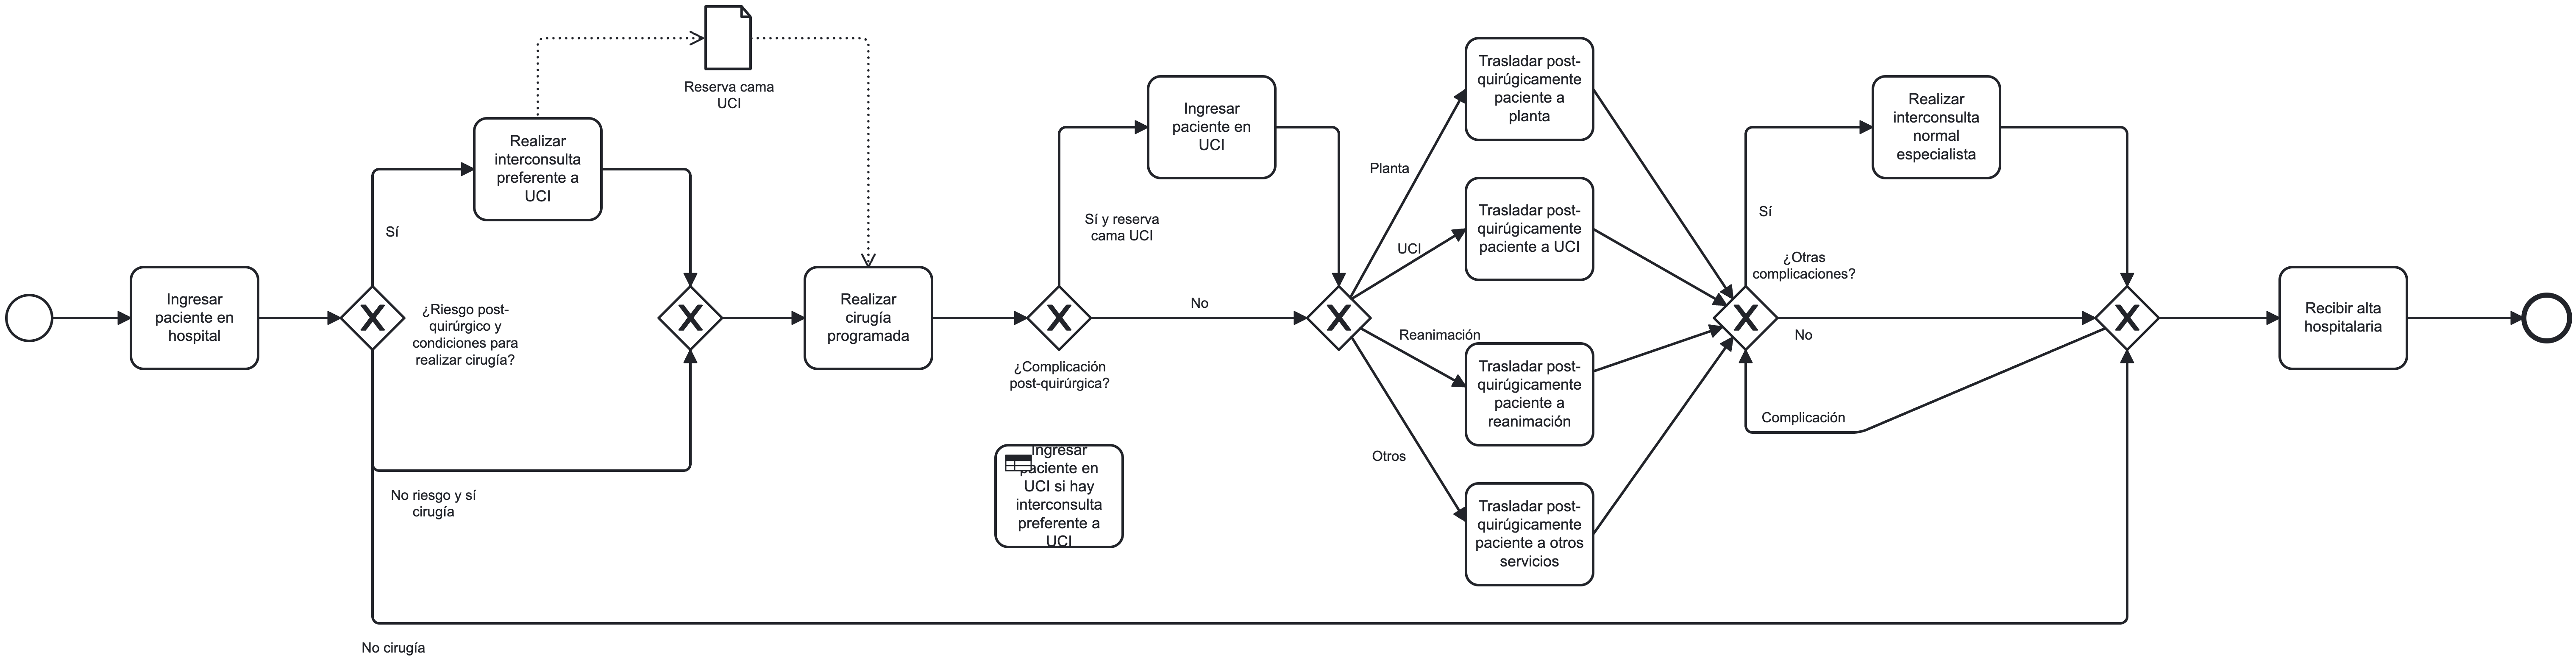
\includegraphics[width=\textheight]{bpmn_proceso_asistencial}
\caption{BPMN reference model of the elective surgical admission process (TO-BE model).}
\label{fig:bpmn}
\end{sidewaysfigure}

\section{Construction of the Event Log}
\label{sec:construccion}

This section describes how the event log was built from the tables of Section~\ref{sec:bd} for the population of Section~\ref{sec:poblacion}: the input and the definition of case and events, the ordering and cleaning of the events, the outputs produced, the two design decisions that shape the event log and the resulting event log.

\subsection{Input, Case and Events}

The event log was generated with a Python script (\code{build\_event\_log\_v3.py}). Its input is the export of the database to CSV files, one file per table with the same name as the table, produced from the PostgreSQL server with semicolon as separator and UTF-8 encoding. The script reads the four event tables of Table~\ref{tab:tablas} (\code{ftr\_hosp}, \code{ftr\_hosp\_interconsultas}, \code{ftr\_hosp\_int\_quirurgicas} and \code{ftr\_hosp\_traslados}), the coding table and the catalogs, and keeps only the episodes of the elective surgical branch.

The case is the hospitalization episode, identified by \code{id\_anonim\_episodio}. The patient code is kept as a case attribute, which allows grouping the episodes of the same patient. Each row of the four event tables is transformed into one or more events according to the rules in Table~\ref{tab:actividades}, which also gives the element of the reference model that each activity represents and the number of events obtained. The activity names are kept in Spanish, as they appear in the source database and in the code. The timestamp of each event is the date and time recorded in its source table. For \code{INGRESO}, \code{ALTA}, \code{EXITUS} and \code{TRASLADO\_OTRO\_HOSPITAL} it is the admission or discharge date. For the consultations it is the date of the consultation. For \code{QUIROFANO\_INICIO} and \code{QUIROFANO\_FIN} it is the start and the end of the intervention. For the \code{DESTINO\_*} activities it is also the end of the intervention, because the surgical table does not record a time of its own for the destination decision. For \code{INGRESO\_UCI} and \code{TRASLADO\_PLANTA} it is the start of the stay in the new bed.

\begin{table}[htbp]
\centering
\caption{Activities of the event log, their origin and their frequency.}
\label{tab:actividades}
\footnotesize
\begin{tabular}{L{4.5cm}L{3.9cm}L{3.6cm}r}
\toprule
Activity & Construction rule & BPMN element (Figure~\ref{fig:bpmn}) & Events \\
\midrule
\code{INGRESO} & Admission date from \code{ftr\_hosp} & Ingresar paciente en hospital & 1,475 \\
\code{INTERCONSULTA\_UCI} & Consultation with target service ICU & Realizar interconsulta preferente a UCI & 18 \\
\code{INTERCONSULTA\_ESPECIALISTA} & Consultation to any other service & Realizar interconsulta normal especialista & 452 \\
\code{QUIROFANO\_INICIO} / \code{FIN} & Start and end of each intervention & Realizar cirugía programada & 1,396 / 1,396 \\
\code{DESTINO\_PLANTA} & \code{codigo\_destino} ward or recovery room & Destination decision: Planta & 1,212 \\
\code{DESTINO\_UCI} & \code{codigo\_destino} ICU & Destination decision: UCI (bed reservation) & 124 \\
\code{DESTINO\_REANIMACION} & \code{codigo\_destino} post-anesthesia care unit & Destination decision: Reanimación & 53 \\
\code{DESTINO\_OTROS} & Home, day surgery unit, emergency care or others & Destination decision: Otros & 7 \\
\code{INGRESO\_UCI} & Actual transfer to the ICU (\code{ftr\_hosp\_traslados}) & Ingresar paciente en UCI & 148 \\
\code{TRASLADO\_PLANTA} & Actual transfer to another unit other than the ICU & Trasladar post-quirúrgicamente paciente a planta & 24 \\
\code{TRASLADO\_OTRO\_HOSPITAL} & Discharge reason: transfer & Not in the model & 1 \\
\code{EXITUS} & Discharge reason: death & Not in the model (discharge reason) & 9 \\
\code{ALTA} & Discharge date, remaining reasons & Recibir alta hospitalaria & 1,465 \\
\bottomrule
\end{tabular}
\end{table}

Two catalogs of the database intervene in the rules of Table~\ref{tab:actividades}: the anesthesia types and the postoperative destinations. Table~\ref{tab:catalogos} lists the codes of both catalogs, one block per catalog, and shows how each code is used: the anesthesia code becomes an attribute of the surgery, and the destination codes are grouped into the four \code{DESTINO\_*} activities. The ward and the recovery room are merged because the recovery room is a transit before the ward; the ICU and the post-anesthesia care unit are kept as destinations of their own; and the remaining destinations (home, day surgery unit, emergency care and others), which are rare, are grouped together.

\begin{table}[htbp]
\centering
\caption{Catalog codes used in the construction of the event log. The anesthesia codes feed a surgery attribute; the destination codes are grouped into the four \code{DESTINO\_*} activities.}
\label{tab:catalogos}
\small
\begin{tabular}{rL{6.0cm}L{5.2cm}}
\toprule
Code & Value & Use in the event log \\
\midrule
\multicolumn{3}{l}{Catalog \code{tipo\_anestesia\_pk} (anesthesia type)} \\
1 & Local & Surgery attribute (anesthesia) \\
2 & General & Surgery attribute (anesthesia) \\
4 & [Sin anestesia] (no anesthesia) & Surgery attribute (anesthesia) \\
5 & Regional & Surgery attribute (anesthesia) \\
6 & [Sin datos] (no data) & Surgery attribute (anesthesia) \\
7 & Gral-UCI (general, ICU destination) & Surgery attribute (anesthesia) \\
8 & Gral-REA (general, post-anesthesia care unit) & Surgery attribute (anesthesia) \\
9 & Sedaci\'on (sedation) & Surgery attribute (anesthesia) \\
\midrule
\multicolumn{3}{l}{Catalog \code{destinos\_postoperatorio\_quirofano} (postoperative destination)} \\
1 & PLANTA (ward) & Activity \code{DESTINO\_PLANTA} \\
2 & DESPERTAR (recovery room) & Activity \code{DESTINO\_PLANTA} \\
7 & UCI (ICU) & Activity \code{DESTINO\_UCI} \\
9 & REANIMACI\'ON (post-anesthesia care unit) & Activity \code{DESTINO\_REANIMACION} \\
3 & DOMICILIO (home) & Activity \code{DESTINO\_OTROS} \\
4 & UCSI (day surgery unit) & Activity \code{DESTINO\_OTROS} \\
5 & OTROS (others) & Activity \code{DESTINO\_OTROS} \\
8 & URGENCIAS (emergency care) & Activity \code{DESTINO\_OTROS} \\
\bottomrule
\end{tabular}
\end{table}

\subsection{Ordering and Cleaning of the Events}

Once the events were created, they were sorted within each case by timestamp. The timestamps of the database have a resolution of one minute, and therefore several events of the same case may share the same minute. This happens mainly at the end of the surgery: \code{QUIROFANO\_FIN} and the \code{DESTINO\_*} event take, by construction, the same timestamp, and in some cases the transfer to the ICU is recorded in the same minute. For these ties a fixed order was applied that reproduces the logic of the process: first the end of the surgery (\code{QUIROFANO\_FIN}), then the destination decision (\code{DESTINO\_*}) and then the actual admission to the ICU (\code{INGRESO\_UCI}). More generally, the tie-break follows the order admission, consultations, operating theater, destination, ICU, transfer and discharge. Without this rule, the order of two events in the same minute would depend on the order of the rows in the source files, and the same situation could produce different traces.

Then the events that fall outside the episode were discarded. An event was kept if its timestamp lies in the interval from one day before the admission date to one day after the discharge date, that is, in [\code{fecha\_ingreso} $-$ 1 day, \code{fecha\_alta} $+$ 1 day]. The one-day margin absorbs the acts recorded just before the admission (for example a preoperative consultation on the previous day) or just after the discharge. Only three events of the whole event log fell outside this interval: the start, the end and the destination of a single intervention whose recorded date is six years before its episode, which is a recording error.

\subsection{Outputs}

The script produces three outputs, each with a use of its own.

\begin{itemize}[leftmargin=*]
  \item \textbf{The event table}, in CSV and Parquet format (\code{eventlog\_pq.csv} and \code{.parquet}): one row per event, with the case, the activity, the timestamp, the attributes inherited from its source row (service, bed, priority, requesting and target service, type, category, approach and anesthesia of the intervention, postoperative destination, discharge reason) and the phase attribute (\code{fase} in the code) described below. This is the input of the PPM experiments of Chapter~\ref{cap:implementacion}, which read the Parquet file with pandas. The CSV copy allows inspecting the data with any tool.
  \item \textbf{The case table} (\code{eventlog\_pq\_casos.csv} and \code{.parquet}): one row per episode with the case attributes of Section~\ref{sec:atributos} and the candidate labels of Section~\ref{sec:etiquetas}. The experiments join it with the event table through the case code to obtain the static vector of each prefix and the label of each case.
  \item \textbf{The XES file} (\code{eventlog\_pq.xes.gz}), the standard format of PM, written with PM4Py. It contains the activities, the timestamps and the light attributes of each event, without missing text values, so that Disco, ProM and Celonis import it without errors. It is the input of the discovery and conformance checking of Section~\ref{sec:discovery}.
\end{itemize}

\subsection{Two Design Decisions}

Two design decisions deserve a detailed explanation, because they determine what the event log can say about the planning of the process and about what actually happened.

The first decision is the \textbf{distinction between planned destination and actual transfer}. The surgical table records, at the end of the operation, the postoperative destination decided by the surgical team: the ward, the ICU, the post-anesthesia care unit or another unit. It is a decision, not a movement, and the table does not even store a time for it. The transfers table, on the other hand, records the physical movement of the patient from one bed to another, with the time at which the new bed was occupied. The two are different and the event log keeps them as different activities: \code{DESTINO\_*} for the decision, with the timestamp of the end of the surgery, and \code{INGRESO\_UCI} or \code{TRASLADO\_PLANTA} for the movement, with its actual time. Version 2 of the event log did not have the \code{DESTINO\_*} activities and recorded only the movements; the decision was visible only as an attribute of the surgery event. Making the decision an activity of its own is what allows comparing, in Section~\ref{sec:destino_uci}, what was planned with what happened. The actual times are kept even when they contradict the expected order: in 34 cases the transfer to the ICU is recorded before the end of the surgery, because the bed in the ICU is assigned while the patient is still in the operating theater. These cases were not corrected, since altering the times would hide a feature of the recording system that conformance checking must detect.

The second decision is the \textbf{phase attribute} (\code{fase} in the code). Each event is labeled with the phase of the episode in which it occurs, computed with respect to the first \code{QUIROFANO\_INICIO} of the case. An event is \emph{preoperative} if it precedes it, \emph{surgery} if it is the start or the end of an intervention, \emph{postoperative} if it follows the first surgery and \emph{without surgery} if the case has no recorded intervention. The event log has 1,472 preoperative, 4,188 surgery, 1,769 postoperative and 351 without-surgery events. This attribute has two uses. In the construction of the prefixes (Section~\ref{sec:prefijos}) it indicates whether the surgery is already in the prefix, and therefore whether the surgery attributes may be used. In the definition of the labels it separates, for example, the ICU consultations before and after the surgery, or the postoperative complication from the preoperative events.

\subsection{The Resulting Event Log}

Table~\ref{tab:resumen_log} summarizes the event log obtained. The dominant variant, \code{INGRESO} $\rightarrow$ \code{QUIROFANO\_INICIO} $\rightarrow$ \code{QUIROFANO\_FIN} $\rightarrow$ \code{DESTINO\_PLANTA} $\rightarrow$ \code{ALTA}, covers 916 cases (62\%). It is followed by the variants with a specialist consultation before, during or after the surgery (186 cases), the admission without recorded surgery (100 of the 142 episodes without a recorded intervention go directly from \code{INGRESO} to \code{ALTA}; the rest have consultations or transfers), the exit to the post-anesthesia care unit (44) and the planned ICU (36). Some episodes have more than one transfer to the ICU, which is why Table~\ref{tab:actividades} counts 148 \code{INGRESO\_UCI} events for the 131 episodes with an ICU admission. Figure~\ref{fig:dfg} shows the complete DFG of the elective surgical process obtained with PM4Py, and Figure~\ref{fig:disco} the frequency map of the same event log in Disco, which draws the same 14 activities and the same transitions with the frequency of each one.

\begin{table}[htbp]
\centering
\caption{Summary of the event log (version 3).}
\label{tab:resumen_log}
\small
\begin{tabular}{L{8cm}r}
\toprule
Measure & Value \\
\midrule
Cases (episodes) & 1,475 \\
Patients & 1,308 \\
Events & 7,780 \\
Activities & 14 \\
Variants & 97 \\
Directly-follows transitions & 59 \\
Events per case: median (minimum, maximum) & 5 (2, 32) \\
Cases with recorded surgery & 1,333 (90.4\%) \\
Cases with more than one intervention & 46 \\
Length of stay in days: median (mean, maximum) & 3.2 (4.9, 195) \\
Admission dates & 1 March 2023 to 29 February 2024 \\
\bottomrule
\end{tabular}
\end{table}

\begin{figure}[htbp]
\centering
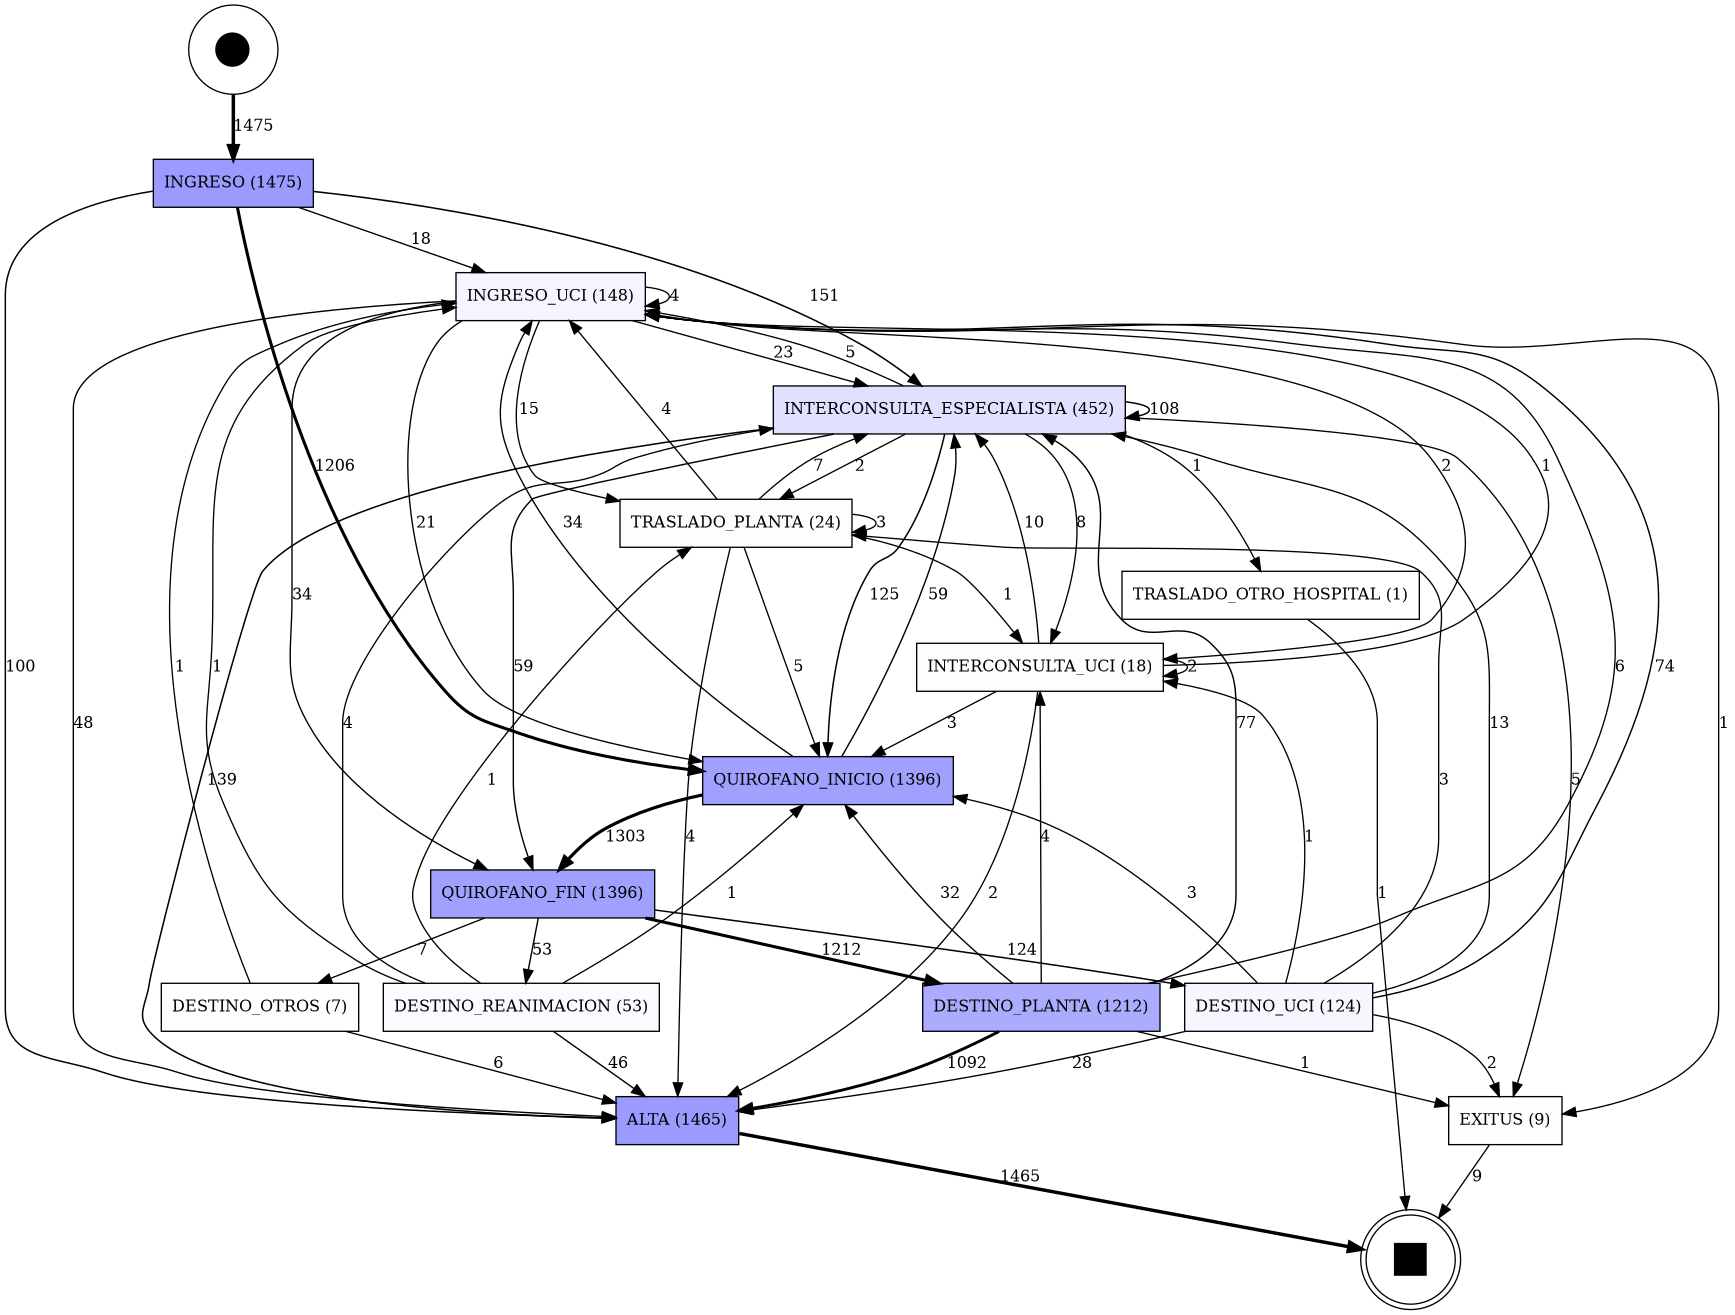
\includegraphics[width=0.85\textwidth]{dfg_v3}
\caption{DFG of the elective surgical process (PM4Py), with the frequency of each activity and of each transition.}
\label{fig:dfg}
\end{figure}

\begin{figure}[htbp]
\centering
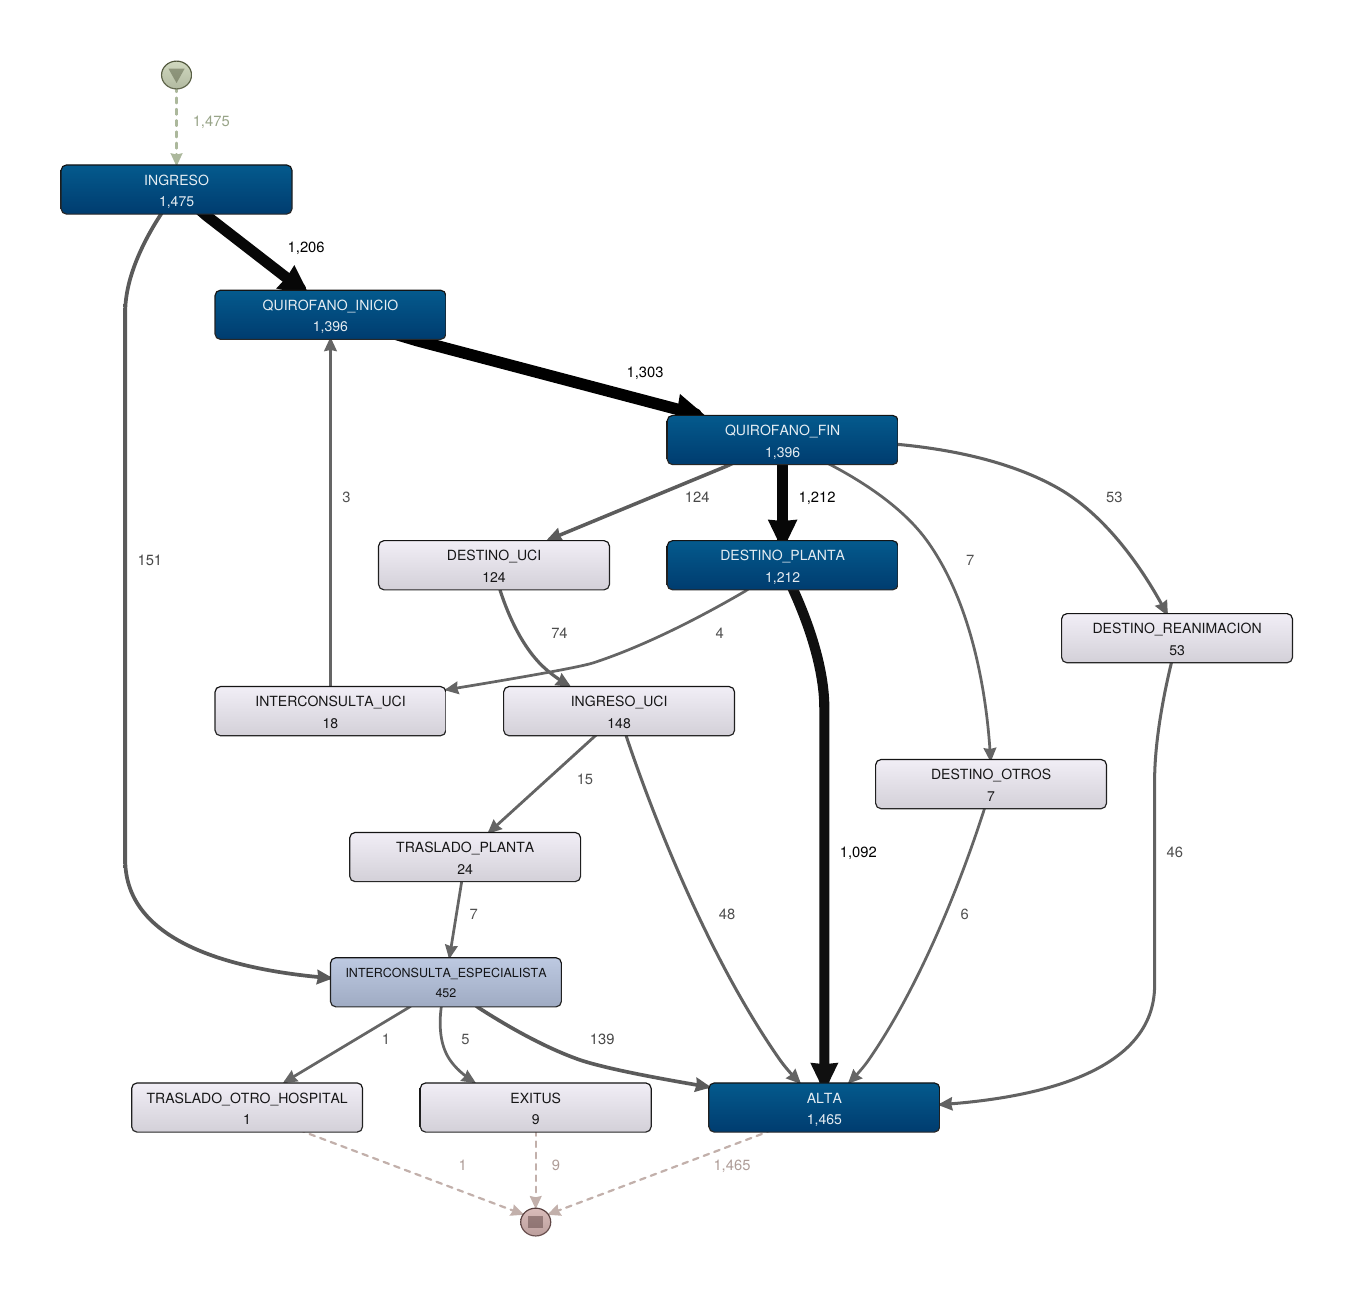
\includegraphics[width=0.95\textwidth]{disco_frecuencia}
\caption{Frequency map of the event log in Disco.}
\label{fig:disco}
\end{figure}

\section{Candidate Outcome Labels}
\label{sec:etiquetas}

The first thing predicted in this work is the \textbf{next activity} of a running case (Prediction~1). This prediction needs no label: the target of each prefix is the activity that follows it in the trace, and it is the prediction addressed by the Entropy-Driven Next Activity Prediction Approach of Zare et al.\ \cite{zare2025}, with which this work is compared.

The outcome-based predictions (Predictions~2 and~3) do need a label per case, and here the work meets a limitation of the data. FTR, as defined in Section~\ref{sec:datos_clinicos}, is the death after a complication that could have been treated. The database does not record whether a complication occurred, whether it was detected or whether the response was adequate. Therefore FTR cannot be labeled directly. What can be done is to define \textbf{candidate labels} from the observable precursors of FTR that the data do record: the admission to the ICU, the prolonged length of stay, the consultations, the death and the transfer to another hospital. Ten binary labels were defined from the case table. Table~\ref{tab:etiquetas} lists them with their number of positive cases and the assessment of their feasibility as a prediction target. The feasibility criterion is the number of positives available for evaluation: with a temporal split in which the 20\% most recent cases form the test set (295 cases), a label with 1\% of positives leaves three positive cases in the test set, which is not enough to measure anything.

\begin{table}[htbp]
\centering
\caption{Candidate outcome labels and their feasibility.}
\label{tab:etiquetas}
\small
\begin{tabular}{L{4.6cm}L{4.6cm}L{1.9cm}L{2.5cm}}
\toprule
Label & Definition & Positives & Feasibility \\
\midrule
\code{label\_ingreso\_uci} & Any \code{INGRESO\_UCI} in the episode & 131 (8.9\%) & Feasible (Prediction~2) \\
\code{label\_estancia\_prolongada} & Length of stay above the 90th percentile (8.74 days) & 148 (10.0\%) & Feasible (Prediction~3) \\
\code{label\_complicacion\_postop} & Postoperative ICU, postoperative specialist consultation, death or transfer & 240 (16.3\%) & Complementary \\
\code{label\_uci\_no\_planificada} & \code{INGRESO\_UCI} without postoperative destination ICU & 21 (1.4\%) & Complementary, with cross-validation \\
\code{label\_ftr\_compuesto} & Death, ICU admission or transfer & 135 (9.2\%) & Redundant with Prediction~2 (131 of 135) \\
\code{label\_reingreso\_7d} & Readmission within 7 days & 23 (1.6\%) & Unfeasible \\
\code{label\_exitus\_intrahosp} & In-hospital death & 9 (0.6\%) & Unfeasible \\
\code{label\_exitus\_30d} / \code{90d} & Death within 30 / 90 days & 10 / 26 & Unfeasible \\
\code{label\_traslado\_otro\_hosp} & Transfer to another hospital & 1 & Unfeasible \\
\bottomrule
\end{tabular}
\end{table}

The labels are read as follows.

\begin{itemize}[leftmargin=*]
  \item \textbf{ICU admission} (\code{label\_ingreso\_uci}) is positive when the episode has at least one actual transfer to the ICU, whatever its moment and whether or not it was planned. With 131 positives (8.9\%) it is feasible and it is the label of \textbf{Prediction~2}. Its relation with the planning of the surgery is analyzed in Section~\ref{sec:destino_uci}.
  \item \textbf{Prolonged length of stay} (\code{label\_estancia\_prolongada}) is positive when the stay exceeds the 90th percentile of the population, 8.74 days. The threshold is a percentile, and not a clinical value, because the expected length of stay depends on the surgery. With 148 positives (10.0\%) it is feasible and it is the label of \textbf{Prediction~3}.
  \item \textbf{Postoperative complication} (\code{label\_complicacion\_postop}) is a broad label: it is positive when, after the surgery, there is an ICU admission, a consultation to a specialist, a death or a transfer. It has the most positives (240, 16.3\%), but it mixes very different situations, from a routine consultation to a death. It is studied as a complementary analysis.
  \item \textbf{Unplanned ICU admission} (\code{label\_uci\_no\_planificada}) is positive when there is an ICU admission and the postoperative destination recorded in the operating theater was not the ICU. It is the label closest to FTR, because it captures the complication that nobody anticipated, but it has only 21 positives (1.4\%). It is studied as a complementary analysis with cross-validation instead of a temporal split, so that no positive case is lost to the split.
  \item \textbf{Composite FTR} (\code{label\_ftr\_compuesto}), positive on death, ICU admission or transfer, is redundant with ICU admission: 131 of its 135 positives are ICU admissions. It is not studied separately.
  \item \textbf{Readmission within 7 days}, \textbf{in-hospital death}, \textbf{death within 30 or 90 days} (computed from \code{fecha\_exitus}) and \textbf{transfer to another hospital} have between 1 and 26 positives. They are unfeasible as prediction targets. Death, the most serious outcome of FTR, is almost nonexistent in elective surgery (0.6\%), which rules out any mortality-based target.
\end{itemize}

In summary, ICU admission and prolonged length of stay are the only outcomes with enough positives for an evaluation with a temporal split. Postoperative complication has even more positives but is heterogeneous, and unplanned ICU admission, the purest clinical target, has only 21 cases.

\section{Planned Destination versus Actual ICU Admission}
\label{sec:destino_uci}

Before predicting the ICU admission, it was checked how it relates to the destination decided in the operating theater. The result, shown in Table~\ref{tab:destino_uci}, is the finding that most conditions the work. The table crosses the postoperative destination recorded for the first intervention of each episode with the actual ICU admission. Of the 110 cases with planned destination ICU, \textbf{all 110 are admitted to the ICU}: the ICU destination is, in practice, the bed reservation. Of the 1,165 cases with destination ward, only 11 end up in the ICU; of the 52 with destination post-anesthesia care unit, two. The \textbf{21 ICU admissions without a planned ICU destination} (11 + 2 + 1 + 7 without surgery) are the \emph{unplanned} ICU admissions, the complication that nobody anticipated: FTR in the strict sense.

\begin{table}[htbp]
\centering
\caption{Planned postoperative destination (first intervention) versus actual ICU admission.}
\label{tab:destino_uci}
\begin{tabular}{lrr}
\toprule
Planned destination & Cases & Admitted to the ICU \\
\midrule
Ward (ward + recovery room) & 1,165 & 11 \\
ICU & 110 & 110 (100\%) \\
Post-anesthesia care unit & 52 & 2 \\
Others (day surgery unit) & 6 & 1 \\
No surgery / no data & 142 & 7 \\
\midrule
\textbf{Total} & \textbf{1,475} & \textbf{131} \\
\bottomrule
\end{tabular}
\end{table}

Two consequences follow from this table. The first affects the reading of the reference model: the `priority consultation to the ICU' that the BPMN model places before the surgery does not exist before the surgery in the data (zero preoperative cases; the 18 ICU consultations recorded are postoperative). The bed reservation of the model materializes in the data as the postoperative destination recorded in the operating theater, and this is how it is read in the conformance checking of Chapter~\ref{cap:implementacion}. The second affects prediction: any model that sees \code{DESTINO\_UCI} in the prefix predicts the ICU admission trivially, because it is reading a decision already taken. Measuring real predictive ability therefore requires hiding that information or changing the target.

This single table gives rise to three ways of asking the question `will the patient be admitted to the ICU?', which differ in the information available to the model and in the population. Figure~\ref{fig:variantes} summarizes them.

\begin{itemize}[leftmargin=*]
  \item \textbf{Variant A: without planning information}. The population is the whole event log (1,475 cases) and the label is the ICU admission (131 positives). The planned destination is removed from the prefixes, and the anesthesia that reveals it (\code{Gral-UCI}, general anesthesia with ICU destination, recorded at the start of the surgery) is recoded as plain general anesthesia. The model must predict the admission with what the patient, the service and the surgery say. This is \textbf{Prediction~2}, the one reported in Chapter~\ref{cap:implementacion} as the main result, because it measures what a model could add to the decision of the surgical team.
  \item \textbf{Variant B: with planning information}. Same population and same label, but the destination and the anesthesia stay in the prefix. The model only has to read them. The result is not a prediction but an \textbf{upper bound}: it measures how much of the ICU admission is already decided in the operating theater, and it serves as a reference for the other two variants.
  \item \textbf{Variant C: unplanned ICU admission}. The population is restricted to the 1,365 cases without a planned ICU destination and the label is the unplanned admission (21 positives). Here the destination is legitimate information, because no positive case has the ICU as destination, and therefore nothing has to be hidden. It is the purest clinical question, but with only 21 positives it is evaluated as a complementary analysis.
\end{itemize}

\begin{figure}[htbp]
\centering
\begin{tikzpicture}[
  ev/.style={draw=black!60, fill=black!5, rounded corners=2pt, font=\tiny\ttfamily, minimum height=4.5mm, inner sep=2.5pt},
  hid/.style={ev, draw=red!70, fill=red!8, text=red!70!black},
  rec/.style={ev, draw=orange!80!black, fill=yellow!25},
  lab/.style={font=\footnotesize, anchor=east, align=right, text width=3.3cm},
  note/.style={font=\scriptsize, anchor=north west, text width=9.2cm, align=left}]
\node[lab] at (-0.2,3.7) {\textbf{A}: Prediction~2\\ 1,475 cases, 131 positives};
\node[ev, anchor=west] (a1) at (0,3.7) {INGRESO};
\node[ev, right=1.5mm of a1] (a2) {QUIROFANO\_INICIO};
\node[rec, right=1.5mm of a2] (a3) {Gral-UCI $\to$ General};
\node[ev, right=1.5mm of a3] (a4) {QUIROFANO\_FIN};
\node[hid, right=1.5mm of a4] (a5) {DESTINO\_UCI};
\node[note] at (0,3.4) {Planning information hidden: the destination is removed and the anesthesia recoded. The model predicts.};
\node[lab] at (-0.2,2.05) {\textbf{B}: upper bound\\ 1,475 cases, 131 positives};
\node[ev, anchor=west] (b1) at (0,2.05) {INGRESO};
\node[ev, right=1.5mm of b1] (b2) {QUIROFANO\_INICIO};
\node[ev, right=1.5mm of b2] (b3) {Gral-UCI};
\node[ev, right=1.5mm of b3] (b4) {QUIROFANO\_FIN};
\node[ev, right=1.5mm of b4] (b5) {DESTINO\_UCI};
\node[note] at (0,1.75) {Planning information visible: the model reads the decision already taken.};
\node[lab] at (-0.2,0.4) {\textbf{C}: unplanned ICU\\ 1,365 cases, 21 positives};
\node[ev, anchor=west] (c1) at (0,0.4) {INGRESO};
\node[ev, right=1.5mm of c1] (c2) {QUIROFANO\_INICIO};
\node[ev, right=1.5mm of c2] (c3) {Gral-REA};
\node[ev, right=1.5mm of c3] (c4) {QUIROFANO\_FIN};
\node[ev, right=1.5mm of c4] (c5) {DESTINO\_PLANTA};
\node[note] at (0,0.1) {Cases with planned destination ICU excluded: no positive has it, and therefore nothing has to be hidden.};
\end{tikzpicture}
\caption{The three variants of the ICU admission question. Each row shows a prefix as the model sees it: the red element is removed from the prefix and the yellow one is recoded.}
\label{fig:variantes}
\end{figure}

Chapter~\ref{cap:implementacion} evaluates the three variants with the same models and the same protocol: variant A as Prediction~2 (Section~\ref{sec:pred2}) and variants B and C as complementary analyses (Sections~\ref{sec:compl_b} and~\ref{sec:compl_c}). Figure~\ref{fig:niveles_abc} in that chapter gives the detail of the implementation of each one.

\section{Warnings About Information Leakage}
\label{sec:fugas}

Information leakage occurs when a model uses, as input, information that would not be available at the moment of the prediction, or that is a consequence of the outcome to be predicted. The planned destination of the previous section is the clearest case. In addition, the following variables of the case table were identified as leakage and excluded from the models.

\begin{itemize}[leftmargin=*]
  \item \textbf{Discharge service} (\code{servicio\_alta}) and \textbf{discharge reason} (\code{motivo\_alta}). They are known at discharge. The reason reveals death and transfer directly, and the service reveals whether the patient was in the ICU at the end.
  \item \textbf{Length of stay} (\code{estancia\_dias}), the difference between the discharge and admission dates. It is the variable from which the label of Prediction~3 is derived, and it is also longer in the cases with ICU admission.
  \item \textbf{Number of events} of the case (\code{n\_eventos}) and \textbf{bed at discharge} (\code{cama\_al\_alta}). The number of events is only known when the case ends and it grows with the complications; the bed at discharge identifies the unit in which the patient ended.
  \item \textbf{Number of coded diagnoses} (\code{n\_diag}), the less obvious one. ICD-10 coding is performed at discharge by the coding unit, which reviews the whole episode and records one diagnosis per condition treated. Complications add diagnoses: the cases with unplanned ICU admission have 11.5 diagnoses on average versus 5.9 for the rest. The variable looks like a comorbidity measure available at admission, but it is in fact a summary of what happened. As shown in Section~\ref{sec:sens_ndiag}, including \code{n\_diag} doubles the apparent performance on the scarcest target, an unmistakable symptom of leakage.
\end{itemize}

The \textbf{ICD chapter of the main diagnosis} (\code{cie\_capitulo}) comes from the same coding, but it is kept with reservations, because in elective surgery the main diagnosis is the condition for which the surgery was scheduled, and it is known at admission.

\section{Process Entropy}
\label{sec:entropia}

The entropy of the event log was computed with the definition of the Entropy-Driven Next Activity Prediction Approach \cite{zare2025}, introduced in Section~\ref{sec:zare}. The computation has three steps. First, every pair of consecutive events of each trace is counted as one directly-follows transition $a \rightarrow b$. The 1,475 traces of the event log produce 6,305 transitions of 59 distinct types. Second, the probability of each transition type is its relative frequency: for example, the most frequent one, \code{QUIROFANO\_INICIO} $\rightarrow$ \code{QUIROFANO\_FIN}, appears 1,303 times, and therefore $p = 1{,}303 / 6{,}305 = 0.207$. Third, the Shannon entropy of this distribution is computed as $H = -\sum_t p(t)\log_2 p(t)$. The four dominant transitions (surgery start to end, surgery end to ward destination, admission to surgery and ward destination to discharge, each with $p$ between 0.17 and 0.21) contribute 1.82 bits, and the other 55 transitions, 27 of them with five occurrences or fewer, contribute 1.57 bits. The total is \textbf{3.39 bits} (3.54 bits if the artificial start and end markers of each trace are included, which adds four transition types).

Version 2 of the event log, the one without the destination activities (Section~\ref{sec:historia_tablas}), had 3.04 bits. Adding the postoperative destination contributes about 0.35 bits, because the operating theater comes to have four exits instead of one. The event log falls in the medium band of the paper, between BPIC 2017 (3.24) and BPIC 2020 Prepaid Travel Cost (3.64), the band in which, according to the authors, classical models should perform close to deep ones. Figure~\ref{fig:entropia} places both versions of the event log on the scale of the paper. This prediction is contrasted with the results of the next chapter.

\begin{figure}[htbp]
\centering
\begin{tikzpicture}
\begin{axis}[
  xbar, bar shift=0pt, width=0.72\textwidth, height=7.4cm, bar width=7pt,
  xmin=0, xmax=5.8, ymin=-0.7, ymax=7.9,
  xlabel={Process entropy (bits)}, xlabel style={font=\small},
  ytick={0,1,2,3,4,5,6,7},
  yticklabels={Sepsis, BPIC 2020 Prepaid Travel Cost, Event log v3 (this work), BPIC 2017, BPIC 2020 Request for Payment, Event log v2 (this work), Road Traffic Fine Management, Helpdesk},
  yticklabel style={font=\footnotesize}, tick label style={font=\footnotesize},
  nodes near coords, nodes near coords style={font=\footnotesize, /pgf/number format/fixed, /pgf/number format/precision=2, /pgf/number format/fixed zerofill},
  axis x line*=bottom, axis y line*=left, clip=false,
  legend style={at={(0.98,0.45)}, anchor=east, font=\footnotesize, draw=black!30}, legend cell align=left]
\addplot[fill=blue!60, draw=blue!60] coordinates {(2.60,7) (2.96,6) (3.21,4) (3.24,3) (3.64,1) (5.07,0)};
\addplot[fill=red!70, draw=red!70] coordinates {(3.04,5) (3.39,2)};
\legend{Zare et al. (2025), This work}
\draw[black!40, dashed] (axis cs:3,-0.7) -- (axis cs:3,7.9);
\draw[black!40, dashed] (axis cs:5,-0.7) -- (axis cs:5,7.9);
\node[font=\footnotesize, black!60] at (axis cs:1.5,7.65) {low ($< 3$ bits)};
\node[font=\footnotesize, black!60] at (axis cs:4.0,7.65) {medium (3--5 bits)};
\node[font=\footnotesize, black!60] at (axis cs:5.4,7.65) {high};
\end{axis}
\end{tikzpicture}
\caption[Process entropy of the two versions of the event log compared with the six event logs of the Entropy-Driven Next Activity Prediction Approach.]{Process entropy of the two versions of the event log of this work compared with the six event logs evaluated in the Entropy-Driven Next Activity Prediction Approach \cite{zare2025}; the dashed lines separate the low, medium and high entropy bands of the paper.}
\label{fig:entropia}
\end{figure}

\chapter{Implementation}
\label{cap:implementacion}

This chapter reports the experimental work. It begins with process discovery and conformance checking of the event log with four tools, which validate the event log and the reference model and reveal the finding that conditions the predictive design. It then describes the PPM experimental design: the experiments and their nomenclature, the prefixes and their cutting rules, the encodings, the split, the models and the metrics. Next, it presents the results of the three predictions carried out: next-activity prediction, ICU admission without planning information and prolonged length of stay. It then presents the complementary analyses and, finally, a comparative synthesis and the contrast with the Entropy-Driven Next Activity Prediction Approach of Zare et al.\ \cite{zare2025}.

\section{Process Discovery and Conformance Checking}
\label{sec:discovery}

Before training any predictive model, the event log was analyzed with the PM techniques of Section~\ref{sec:pm}, with two aims: to validate the event log and the reference model, and to understand the process as it is recorded in the data. The work was carried out with four tools: ProM\footnote{\url{https://promtools.org/}}, Disco\footnote{\url{https://fluxicon.com/disco/}}, Celonis\footnote{\url{https://www.celonis.com/}} and PM4Py\footnote{\url{https://processintelligence.solutions/pm4py}}. This section is organized in four parts. Section~\ref{sec:cuatro_herramientas} describes the loading of the event log in the four tools and the reading of the discovered process with the visual tools, Disco and Celonis. Section~\ref{sec:descubiertos} applies two discovery algorithms, the Heuristics Miner and the Inductive Miner, in ProM and PM4Py, to see which one produces the best model of the event log. Section~\ref{sec:conformance} checks the event log against the reference model of Section~\ref{sec:modelo}. Section~\ref{sec:aporte_discovery} collects what this analysis contributes to the predictive design.

\subsection{The Event Log in the Four Tools}
\label{sec:cuatro_herramientas}

The XES file of the event log was loaded into ProM, Disco, Celonis and PM4Py. The four tools read 1,475 cases, 7,780 events and 14 activities; Disco and PM4Py also agree on 97 variants and 59 arcs of the DFG, and on a median case duration of 3.2 days (mean 4.9). This agreement validates the event log as a common input and rules out formatting errors or misinterpretation of the timestamps. The two visual tools give the first reading of the process. The frequency map of Disco (Figure~\ref{fig:disco}, in Chapter~\ref{cap:datos}) shows the dominant path through the operating theater and the ward destination, and the secondary paths through the consultations, the post-anesthesia care unit and the ICU. The Process Explorer of Celonis (Figure~\ref{fig:celonis}) shows the same 14 activities with their case frequencies and allows filtering the cases by variant, which was used to inspect the atypical trajectories one by one.

\begin{figure}[htbp]
\centering
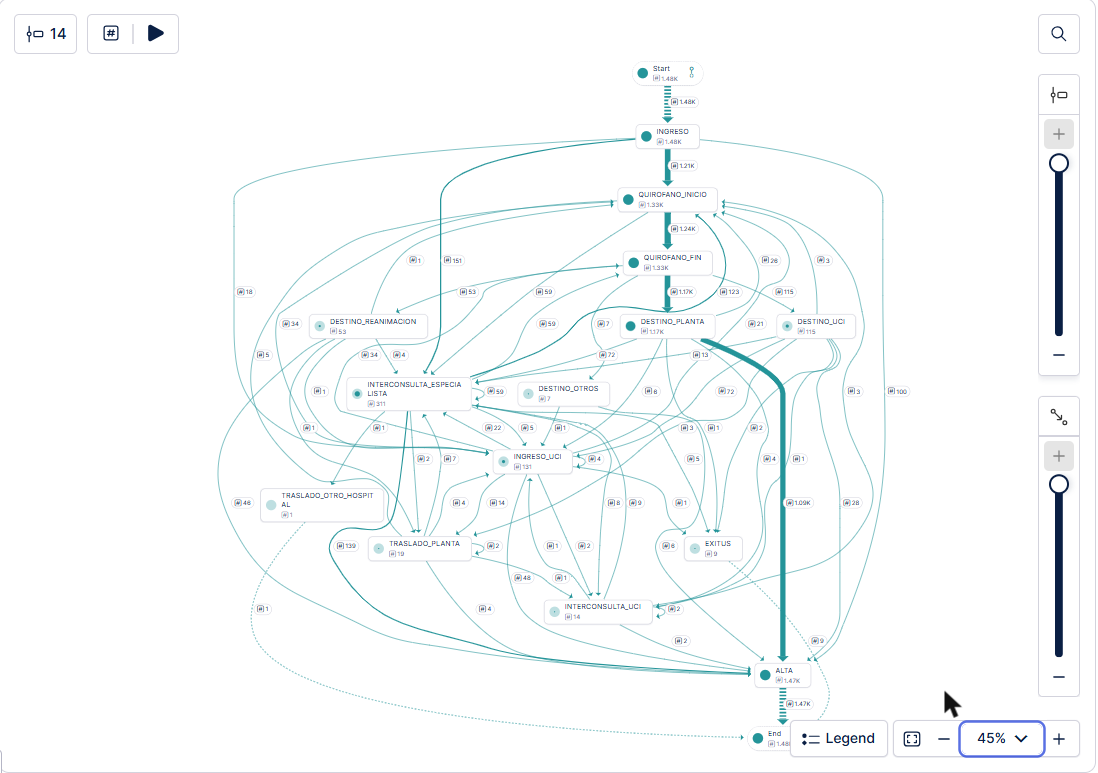
\includegraphics[width=0.9\textwidth]{celonis_explorer}
\caption{Process Explorer of Celonis with the 14 activities of the event log.}
\label{fig:celonis}
\end{figure}

\subsection{Discovered Models}
\label{sec:descubiertos}

Two discovery algorithms were applied, each in two tools, ProM and PM4Py, so that the results could be compared between independent implementations. The Heuristics Miner was run with a dependency threshold of 0.9, which keeps only the transitions that appear in a stable way and filters the infrequent ones; the Inductive Miner was run in its infrequent variant with a noise threshold of 0.2, which guarantees a sound model at the cost of generalizing more. These are the two algorithms described in Section~\ref{sec:pm} and the thresholds are the usual starting values of both tools. Their quality was measured with alignments against the complete event log (Table~\ref{tab:discovery}).

\begin{table}[htbp]
\centering
\caption{Quality of the discovered models (alignments against the event log).}
\label{tab:discovery}
\begin{tabular}{lccc}
\toprule
Model & Fitness & Fitting traces & Precision \\
\midrule
Heuristics Miner, dependency 0.9 (PM4Py) & \textbf{0.972} & 89.9\% & \textbf{0.915} \\
Heuristics Miner (iDHM), dependency 0.9 (ProM) & \textbf{0.984} & -- & -- \\
Inductive Miner infrequent 0.2 (PM4Py) & 0.917 & 76.1\% & 0.510 \\
Inductive Miner infrequent 0.2 (ProM) & 0.912 & -- & -- \\
\bottomrule
\end{tabular}
\end{table}

The Heuristics Miner (Figure~\ref{fig:heuristics}) is the best discovered model in both tools: it represents three of the four exits of the operating theater (\code{DESTINO\_OTROS}, with seven events, is discarded) and the step \code{DESTINO\_UCI} $\rightarrow$ \code{INGRESO\_UCI}, and discards the infrequent activities. ProM, with its reference implementation, the iDHM (Figure~\ref{fig:prom}), reproduces the result with the same thresholds. The Inductive Miner, on the other hand, loses precision. In 34 ICU admissions the actual transfer has a timestamp earlier than the end of the surgery (21 of them form the variant \code{QUIROFANO\_INICIO} $\rightarrow$ \code{INGRESO\_UCI} $\rightarrow$ \code{QUIROFANO\_FIN} $\rightarrow$ \code{DESTINO\_UCI} $\rightarrow$ \code{ALTA}). To cover that order, the algorithm takes the ICU branch out of the surgical block and makes it concurrent, which admits much more behavior than appears in the event log.

\begin{figure}[htbp]
\centering
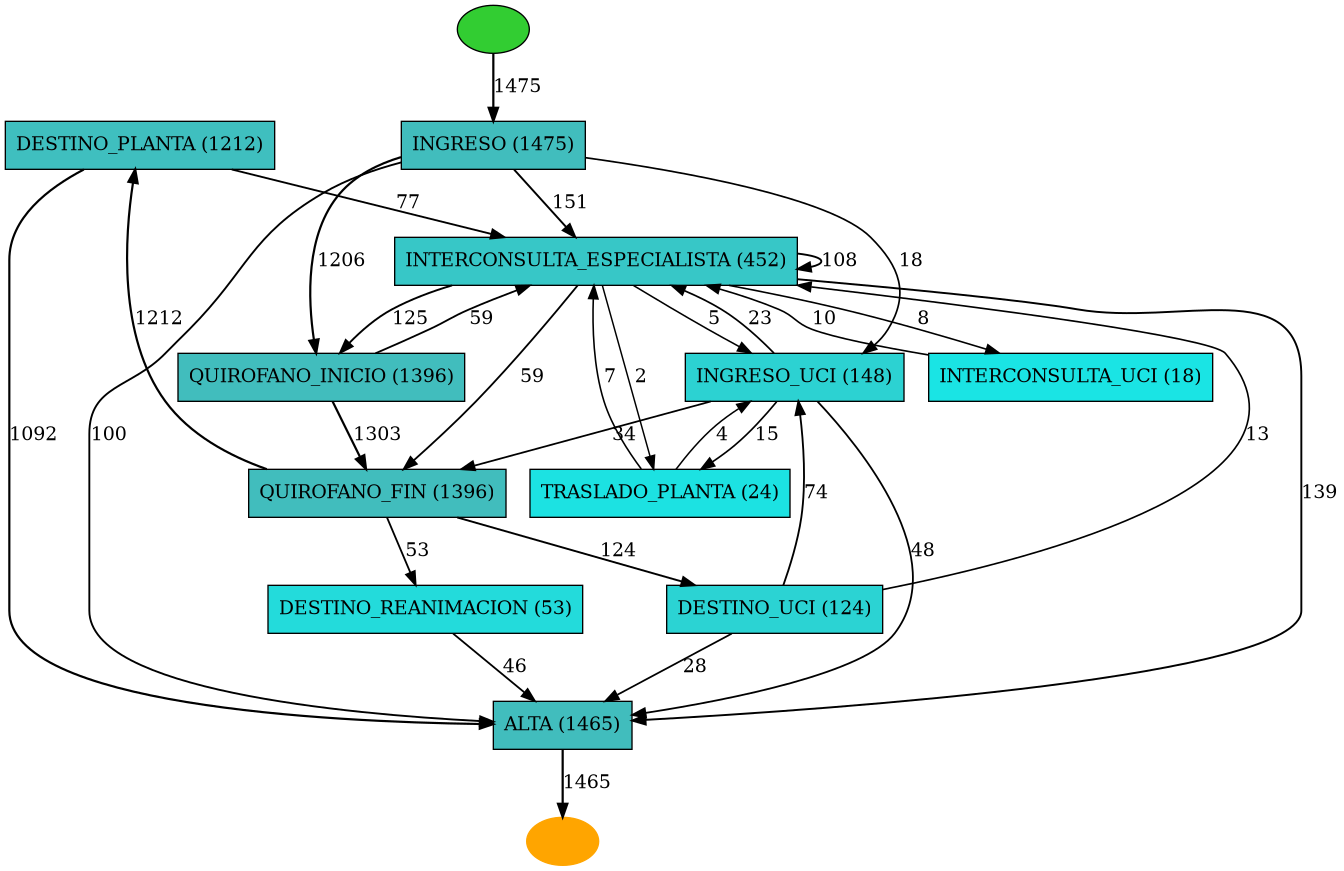
\includegraphics[width=0.9\textwidth]{pm4py_heuristics}
\caption{Heuristic net discovered by PM4Py (dependency 0.9).}
\label{fig:heuristics}
\end{figure}

\begin{figure}[htbp]
\centering
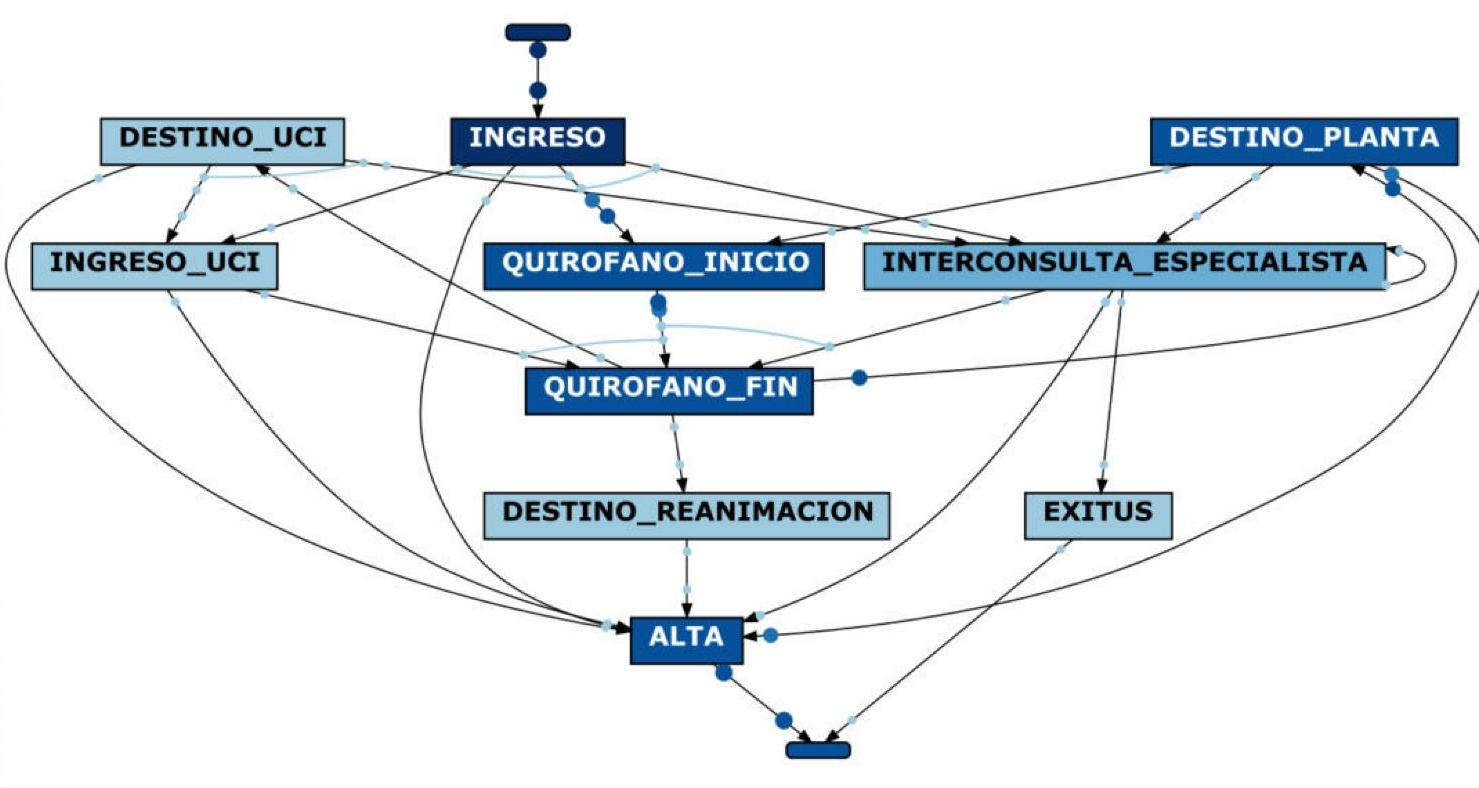
\includegraphics[width=0.9\textwidth]{prom_idhm}
\caption{iDHM in ProM Lite with the same thresholds.}
\label{fig:prom}
\end{figure}

\subsection{Conformance Checking Against the Reference Model}
\label{sec:conformance}

The event log was checked against the reference model of Section~\ref{sec:modelo} (Figure~\ref{fig:bpmn}). For the replay, the tasks of the model were mapped to the activities of the event log as in Table~\ref{tab:actividades}, with one reading imposed by the data (Section~\ref{sec:destino_uci}): the ICU bed reservation of the model corresponds to the ICU destination recorded in the operating theater (\code{DESTINO\_UCI}), which follows the surgery and precedes the ICU admission. The check was made in two tools. In PM4Py, the BPMN model was converted into a Petri net and aligned with the event log: the model reaches a fitness of 0.951 with \textbf{80.9\%} of fitting traces and a precision of 0.639. In the Process Adherence Manager of Celonis, which maps the tasks of the BPMN model to the activities of the event log and counts the cases without deviations, \textbf{80.95\%} of the cases conform (Figure~\ref{fig:celonis_conf}). The agreement between two independent implementations validates the model as the reference of the work.

\begin{figure}[htbp]
\centering
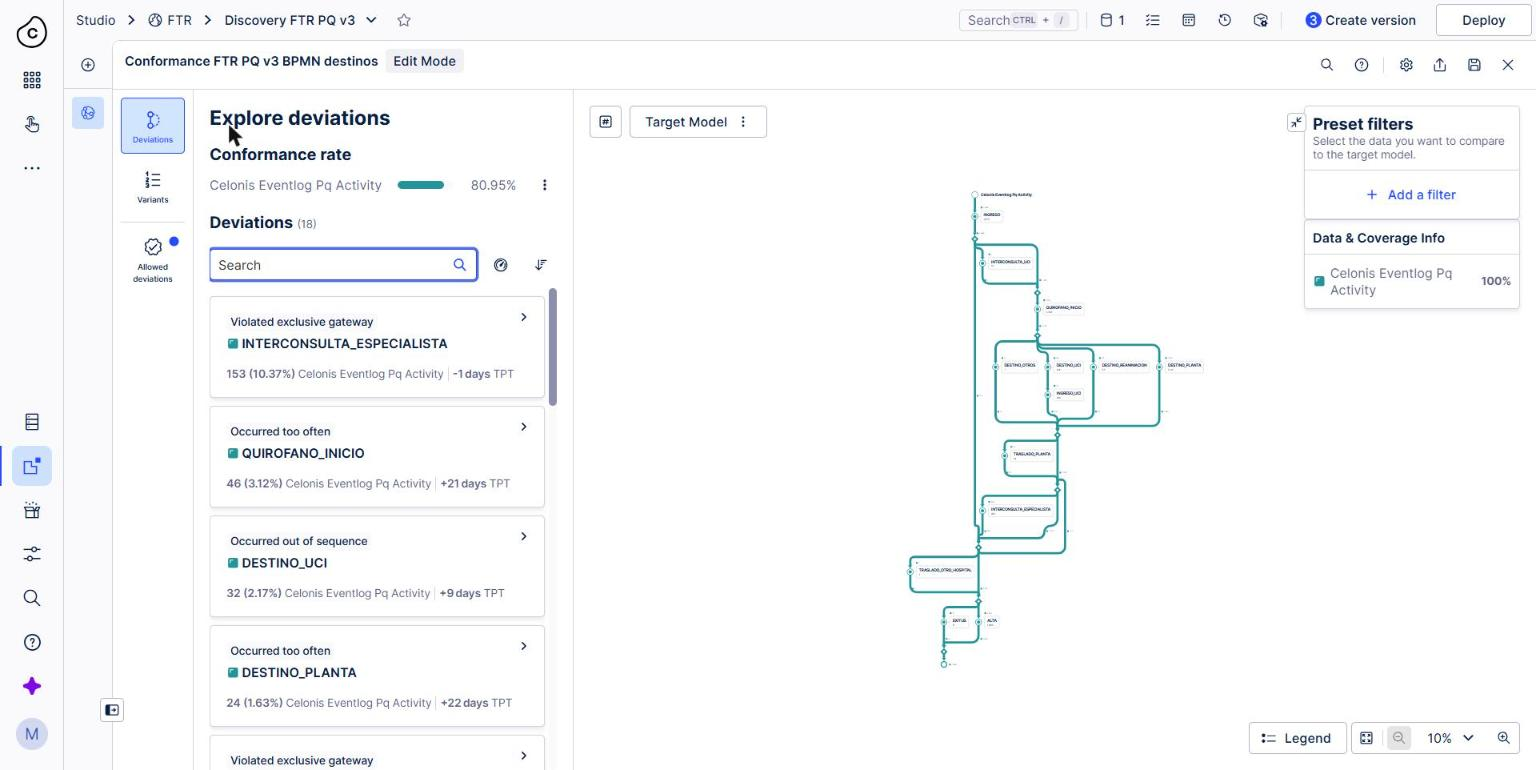
\includegraphics[width=0.85\textwidth]{celonis_conformance}
\caption{Conformance of the event log against the reference BPMN model in the Process Adherence Manager of Celonis (80.95\%).}
\label{fig:celonis_conf}
\end{figure}

The 19\% of cases that do not conform are informative, because their deviations are the behavior that the planned process does not foresee. Three deviations account for most of them.

\begin{itemize}[leftmargin=*]
  \item \textbf{Transfer to the ICU recorded before the destination} (32 cases). Source: the alignments of PM4Py (32 of the 34 transfers of Section~\ref{sec:construccion}; the other two traces are explained by the alignment through another deviation), which report an \code{INGRESO\_UCI} move present in the event log but not allowed by the model at that point. These are the cases of Section~\ref{sec:construccion} in which the ICU bed is occupied while the patient is still in the operating theater, and therefore the actual transfer precedes the end of the surgery and the destination decision.
  \item \textbf{Repeated destinations in reinterventions} (24 cases). Source: the alignments of PM4Py. The model has a single surgery task and a single destination decision, whereas the episodes with two or more interventions record a destination after each one.
  \item \textbf{ICU admission after a ward destination} (20 cases). Source: the Process Adherence Manager of Celonis, which flags it as a violation of the exclusive destination gateway: the case takes the ward branch (\code{DESTINO\_PLANTA}) and then executes \code{INGRESO\_UCI}, which belongs to the ICU branch. The count covers all the interventions of the episode, whereas Table~\ref{tab:destino_uci} considers only the first one, which is why it does not coincide exactly with the 21 unplanned admissions.
\end{itemize}

The third deviation is precisely the unplanned ICU admission: the normative model naturally identifies it as a breach of what was planned.

\subsection{What Discovery Contributes to the Predictive Design}
\label{sec:aporte_discovery}

The findings from the process discovery and conformance checking phases informed the selection of relevant variables, the identification of feasible prediction tasks and the subsequent design of the predictive experiments. Three of them pass directly into the experimental design and are explained below.

First, the postoperative destination ICU anticipates the ICU admission in 100\% of the cases (Table~\ref{tab:destino_uci}). A model that sees \code{DESTINO\_UCI} in the prefix does not predict anything: it reads a decision that the surgical team has already taken and recorded. Its results would measure the consistency of the recording system, not the ability to anticipate a complication. For this reason, the planned destination is removed from the prefixes of Prediction~2, and it is kept only in the complementary analysis B, whose purpose is to measure how much of the admission is decided in the operating theater.

Second, when the planned destination was the ward, the ICU admission arrives with a median of 2.1 days after the operating theater, versus 15 minutes when the ICU was planned. This provides a time horizon in which a prediction would have clinical value: there is time to act between the exit of the operating theater and the deterioration.

Third, the anesthesia recorded at the start of the surgery also reveals the planning. The catalog of anesthesia types of the database distinguishes, within general anesthesia, the values \code{Gral-UCI} and \code{Gral-REA}: general anesthesia for a patient who will be sent to the ICU, or to the post-anesthesia care unit, after the surgery. These values are recorded with \code{QUIROFANO\_INICIO}, that is, before the destination decision, and \code{Gral-UCI} ends in \code{DESTINO\_UCI} in 88 of 122 interventions. The anesthesia therefore anticipates almost the same as the destination and one event earlier. It must be treated in the same way: in Prediction~2 both values are recoded as plain general anesthesia.

\section{Predictive Process Monitoring Experimental Design}

The predictive part of the work follows a single pipeline, summarized in Figure~\ref{fig:pipeline}, which is identical for the three predictions and for the complementary analyses. The event log is cut into prefixes, each prefix is encoded in two ways, the cases are split temporally, the models are trained with three seeds each, and the results are evaluated with metrics suited to each prediction type. The following subsections describe each stage.

The whole experiment is implemented in Python and runs with a single script, \code{run\_final\_v3.py}. The script loads the event table and the case table of the event log, computes the process entropy, builds the prefixes of each prediction with its cutting rule, encodes them, splits the cases temporally, trains the five models with three seeds each and writes the results. It reuses two modules: \code{ppm\_data\_v3.py}, which contains the loading of the event log, the construction of the prefixes, the encodings and the temporal split, and \code{run\_experiments\_v3.py}, which contains the models, the training loop of the neural networks, the metrics and the figures. One complete run of the three predictions takes 551 s on a two-core CPU, without a graphics processing unit, which shows the modest size of the problem. The run leaves in a results folder the metric tables in CSV format, one row per model and seed, the ROC and precision--recall curves, the AUC-ROC per prefix length, the variable importances and an execution log with every figure reported in this chapter. Every table and figure of the chapter can therefore be regenerated from the event log with one command, and the complementary analyses are run with the same modules and different arguments.

\begin{figure}[htbp]
\centering
\begin{tikzpicture}[
  stage/.style={draw=black!60, rounded corners=3pt, fill=black!4, text width=2.38cm, minimum height=3.9cm, align=left, font=\footnotesize, inner sep=5pt, anchor=north},
  num/.style={circle, fill=black!75, text=white, font=\scriptsize\bfseries, minimum size=4.2mm, inner sep=0pt},
  arr/.style={-{Latex[length=2mm]}, thick, black!60}]
\node[stage] (s1) at (0,0) {\hspace*{5.5mm}\textbf{Prefixes}\\[4pt] Trace up to event $k$, $k = 1 \ldots 6$. Never ends in \code{ALTA}, \code{EXITUS} or a transfer to another hospital; cut before the event that defines the label.};
\node[stage, right=0.45cm of s1.north east, anchor=north west] (s2) {\hspace*{5.5mm}\textbf{Encodings}\\[4pt] Aggregate (59--61 variables) for the tree-based models; sequence (embedding + two temporal features + static vector) for LSTM and Transformer.};
\node[stage, right=0.45cm of s2.north east, anchor=north west] (s3) {\hspace*{5.5mm}\textbf{Temporal split}\\[4pt] By admission date, at case level: 64\% training, 16\% validation, 20\% test (the 295 most recent cases).};
\node[stage, right=0.45cm of s3.north east, anchor=north west] (s4) {\hspace*{5.5mm}\textbf{Models}\\[4pt] Five models $\times$ three seeds, basic configuration, no tuning. Threshold chosen on validation (maximum F1-score); early stopping on validation.};
\node[stage, right=0.45cm of s4.north east, anchor=north west] (s5) {\hspace*{5.5mm}\textbf{Metrics}\\[4pt] Outcome: AUC-ROC and AUC per prefix, AUC-PR, Brier, F1-score, recall, precision. Next activity: accuracy and macro F1-score.};
\foreach \i/\n in {s1/1,s2/2,s3/3,s4/4,s5/5} \node[num] at ([xshift=4.2mm,yshift=-4.2mm]\i.north west) {\n};
\foreach \a/\b in {s1/s2,s2/s3,s3/s4,s4/s5} \draw[arr] ([yshift=-1.95cm]\a.north east) -- ([yshift=-1.95cm]\b.north west);
\end{tikzpicture}
\caption{The experimental pipeline, common to the three predictions and to the complementary analyses.}
\label{fig:pipeline}
\end{figure}

\subsection{The Experiments and their Nomenclature}

Six experiments were defined. Three of them are the predictions of the work, named according to the classification of Section~\ref{sec:ppm}: Prediction~1 is a next event prediction (the next activity of the case), and Predictions~2 and~3 are outcome-based predictions with a boolean outcome (ICU admission and prolonged length of stay). The other three are complementary analyses that justify the design of Prediction~2. In the code and in the intermediate reports the six experiments are identified by letters: F is Prediction~1, A is Prediction~2, E is Prediction~3, and B, C and D are the complementary analyses. Each outcome-based experiment combines a label with a rule about the information visible in the prefix. Table~\ref{tab:logica} summarizes the rationale of each one: which label it predicts, which information the model sees, what it measures and how it differs from the others.

\begin{table}[htbp]
\centering
\caption{The six experiments: label, visible information, purpose and difference from the others.}
\label{tab:logica}
\footnotesize
\begin{tabular}{L{0.6cm}L{1.9cm}L{2.2cm}L{3.0cm}L{2.7cm}L{2.6cm}}
\toprule
Exp. & Prediction & Label & What the model sees in the prefix & What it measures & Differs from \\
\midrule
F & \textbf{Prediction 1} & Next activity (13 classes) & Trace up to event $k$; event $k+1$ is predicted & How much of the flow is predictable; the prediction of Zare et al. & A--E: multiclass; it measures the process, not the patient \\
\addlinespace
A & \textbf{Prediction 2} & ICU admission (131) & Trace up to before the first \code{INGRESO\_UCI}, without \code{DESTINO\_*}; anesthesia \code{Gral-UCI}/\code{Gral-REA} recoded as General & Real predictive ability with patient, service and surgery, before anyone decides & B: same label and cut; A hides the planning decision \\
\addlinespace
E & \textbf{Prediction 3} & Length of stay $>$ 8.74 days (148) & Complete trace with \code{DESTINO\_*}; without the prefixes that already exceed the threshold & Resource outcome; classic PPM target & A--D: another question; cut by time, not by event \\
\addlinespace
B & Comple\-mentary & ICU admission & As A, with \code{DESTINO\_*} and the original anesthesia & Upper bound: how much is decided in the operating theater. Not a prediction & A: only in the information. If B $\gg$ A, the difference is planning \\
\addlinespace
C & Comple\-mentary & Unplanned ICU (21) & Only the 1,365 cases without \code{DESTINO\_UCI}; with \code{DESTINO\_*} (no positive has it) & Anticipate the ICU that nobody foresaw: strict FTR & A and B: the label and the population change; the destination is no longer leakage \\
\addlinespace
D & Comple\-mentary & Postoperative complication (240) & Up to before the first postoperative event defining the label; without \code{DESTINO\_*} & FTR in the broad sense, with more positives & A: broader and more heterogeneous label (consultations) \\
\bottomrule
\end{tabular}
\end{table}

Variants A, B and C should be read together, because they are three ways of asking the same question, whether the patient will be admitted to the ICU, with three levels of information, as Figure~\ref{fig:niveles_abc} shows. In A the model sees the admission, the surgery with its anesthesia recoded and the end of the surgery, but not the planned destination: it measures real predictive ability. In B the model also sees the destination, which reveals the label in the 110 planned cases: it measures how much of ICU admission is decided in advance, and it is therefore an upper bound rather than a prediction. In C the population changes to the 1,365 cases without a planned ICU destination and the label to the 21 unplanned admissions; the destination is then legitimate information, because no positive case has it, and the variant measures the ability to anticipate the admission that nobody foresaw, which is FTR in the strict sense.

\begin{figure}[htbp]
\centering
\begin{tikzpicture}[
  ev/.style={draw=black!50, rounded corners=2pt, text width=2.2cm, minimum height=1.0cm, align=center, font=\scriptsize, inner sep=2pt},
  vis/.style={ev, fill=green!12}, rec/.style={ev, fill=yellow!35}, hid/.style={ev, fill=black!12, text=black!45}, rev/.style={ev, fill=red!18}, lab/.style={ev, fill=blue!12, draw=blue!60, very thick},
  rowlab/.style={font=\footnotesize, align=left, text width=3.0cm},
  hdr/.style={font=\tiny\bfseries, align=center, text width=2.3cm}]
% headers
\foreach \x/\h in {0/{\code{INGRESO}},2.4/{\code{QUIROFANO\_INICIO}\\(anesthesia)},4.8/{\code{QUIROFANO\_FIN}},7.2/{\code{DESTINO\_*}},9.6/{\code{INGRESO\_UCI}}} \node[hdr] at (\x,0) {\h};
% row A
\node[rowlab, anchor=east] at (-1.4,-1.15) {\textbf{A}: Prediction~2\\without planning};
\node[vis] at (0,-1.15) {visible};
\node[rec] at (2.4,-1.15) {recoded\\{\tiny\code{Gral-UCI}/\code{Gral-REA} $\to$ General}};
\node[vis] at (4.8,-1.15) {visible};
\node[hid] at (7.2,-1.15) {removed};
\node[lab] at (9.6,-1.15) {label\\(131 cases)};
% row B
\node[rowlab, anchor=east] at (-1.4,-2.4) {\textbf{B}: complementary\\with planning};
\node[vis] at (0,-2.4) {visible};
\node[vis] at (2.4,-2.4) {visible\\{\tiny(original anesthesia)}};
\node[vis] at (4.8,-2.4) {visible};
\node[rev] at (7.2,-2.4) {reveals the label\\{\tiny\code{DESTINO\_UCI} $\Rightarrow$ ICU}};
\node[lab] at (9.6,-2.4) {label\\(131 cases)};
% row C
\node[rowlab, anchor=east] at (-1.4,-3.65) {\textbf{C}: complementary\\unplanned ICU};
\node[vis] at (0,-3.65) {visible};
\node[vis] at (2.4,-3.65) {visible};
\node[vis] at (4.8,-3.65) {visible};
\node[vis] at (7.2,-3.65) {visible\\{\tiny(no positive has \code{UCI})}};
\node[lab] at (9.6,-3.65) {label\\(21 of 1,365 cases)};
% legend
\foreach \x/\s/\t in {0.4/vis/visible, 2.35/rec/recoded, 4.3/hid/hidden, 6.25/rev/{reveals label}, 8.2/lab/label}
  \node[\s, text width=1.6cm, minimum height=0.45cm, inner sep=1pt] at (\x,-4.75) {\t};
\end{tikzpicture}
\caption{The three ways of asking whether the patient will be admitted to the ICU: what the model sees in the prefix in variants A, B and C.}
\label{fig:niveles_abc}
\end{figure}

The design also makes explicit how the Entropy-Driven Next Activity Prediction Approach \cite{zare2025} is transferred to this work (Table~\ref{tab:zare_traslado}). Three elements are kept unchanged: the five algorithms, the process entropy as the measure that characterizes the event log, and next-activity prediction as the reference prediction, which allows a direct comparison with the results table of the paper. One element is added: the two outcome-based predictions that answer the clinical question of the project, which the paper does not address.

\begin{table}[htbp]
\centering
\caption{How the Entropy-Driven Next Activity Prediction Approach of Zare et al.\ is transferred to this work.}
\label{tab:zare_traslado}
\small
\begin{tabular}{L{3.4cm}L{10.2cm}}
\toprule
Element & In this work \\
\midrule
Same algorithm families & DT, RF, XGBoost, LSTM and Transformer, with basic configuration and without hyperparameter search (the paper uses CNN-LSTM and CNN-BiLSTM networks and its own DAW-Transformer). \\
Same measure of the event log & Process entropy: 3.39 bits (3.54 with start and end markers), in the medium band of the paper (Section~\ref{sec:entropia}). \\
Same prediction & Prediction~1 (F), next-activity prediction, comparable with the results table of the paper. \\
Added & Predictions~2 (A) and 3 (E), ICU admission without planning information and prolonged length of stay: the outcome-based predictions that answer the clinical question (FTR), which the paper does not cover. \\
\bottomrule
\end{tabular}
\end{table}

\subsection{Prefixes and Cutting Rules}
\label{sec:prefijos}

The models do not predict from complete traces but from prefixes, because the purpose of PPM is to predict while the case is still running. A prefix is the trace of an episode up to its $k$-th event, with $k = 1 \ldots 6$; the median of the event log is five events, and therefore six prefixes cover practically the whole history of each case. Each prefix is a prediction instance: with $k=1$ the prediction is made at the time of admission, with $k=3$ just after the operating theater. To avoid leakage, no prefix ends in \code{ALTA}, \code{EXITUS} or \code{TRASLADO\_OTRO\_HOSPITAL}, and each prediction cuts the trace \emph{before the event that defines its label}. The cutting rule is therefore specific to each prediction, because the event that reveals the label is different in each case:

\begin{itemize}[leftmargin=*]
  \item \textbf{Prediction~1 (F)}: $k = 1 \ldots \min(n-1, 6)$ and the class is activity $k+1$.
  \item \textbf{Prediction~2 (A)}: before the first \code{INGRESO\_UCI}. The \code{DESTINO\_*} events are removed and the anesthesia \code{Gral-UCI} or \code{Gral-REA} is recoded as General, because both are the decision to reserve a bed.
  \item \textbf{Prediction~3 (E)}: the prefix does not end in an end event and is discarded when the time elapsed since admission already exceeds 8.74 days, because at that point the label is known. No intermediate event is leakage for the length of stay, and therefore all of them are kept, destination included.
  \item \textbf{Complementary analysis D}: before the first postoperative \code{INGRESO\_UCI} or specialist consultation (\code{INTERCONSULTA\_ESPECIALISTA}), \code{EXITUS} or \code{TRASLADO\_OTRO\_HOSPITAL}; preoperative consultations are kept.
\end{itemize}

After applying these rules, Prediction~1 yields 6,013 prefixes with 13 possible classes; Prediction~2, 4,457 prefixes, of which 334 belong to cases that end in the ICU (the positives); and Prediction~3, 5,987 prefixes, of which 721 belong to cases with a prolonged stay. The number of prefixes is larger than the number of cases because each case contributes up to six prefixes, one per prediction point.

\subsection{Encodings}

A prefix is a sequence of events with heterogeneous attributes, and each family of models needs it in a different form: the tree-based models need a fixed-length numeric vector, whereas the neural networks can consume the sequence itself. For this reason the two usual encodings of PPM, introduced in Section~\ref{sec:ppm}, were used. The \textbf{aggregate} encoding, for the tree-based models, produces a vector of 59 to 61 variables. It contains, for each of the 14 activities, its count in the prefix and whether it is the last one; the time elapsed since admission and since the previous event; the case attributes known at admission (age, sex, palliative care, hour and day of the week of admission, the eight most frequent services and the eight most frequent ICD chapters as indicators); and the surgery attributes (category, approach, anesthesia and duration) only when the operating theater is already in the prefix. The \textbf{sequence} encoding, for LSTM and Transformer, keeps the sequence of activities as embeddings with two temporal features per event (logarithm of the time since admission and since the previous event), padded to six positions, and concatenates the same static case vector before the output layer. The next subsection describes this second encoding in detail, because it determines what the sequence models can and cannot learn.

\subsection{Event Encoding for the Sequence Models}
\label{sec:encoding}

The sequence models do not receive the 59--61 aggregate variables but a tensor of fixed shape, six positions by $d$ values, built as Figure~\ref{fig:encoding} shows. Three transformations are involved: homogenizing the length of the prefixes, merging the heterogeneous attributes of each event into a single vector, and keeping the static attributes of the case apart from the sequence.

\paragraph{Length.} Prefixes have between one and six events. All of them are padded to six positions with the reserved activity code 0 and zero temporal features, so that every prefix is a tensor of the same size. In the Transformer, the padding positions are excluded from the attention through a key padding mask and from the final pooling, and therefore a prefix of two events and a prefix of six events yield comparable representations; in the LSTM, the padding is simply read as a neutral token.

\paragraph{Event representation.} In the Transformer each event $i$ of the prefix is represented by a vector $h_i \in \mathbb{R}^{32}$ that is the sum of three learned vectors, as Equation~\ref{eq:encoding} shows:
\begin{equation}
  h_i = \mathrm{Emb}(a_i) + W x_i + p_i .
  \label{eq:encoding}
\end{equation}
The first term is the \textbf{activity embedding}. The activity is first mapped to an integer according to the fixed list of the 14 activities of the event log, from 1 for \code{INGRESO} to 14 for \code{ALTA}. That integer indexes a $15 \times 32$ table whose rows are initialized at random and adjusted by backpropagation. It is not a one-hot encoding: the network learns which 32 numbers represent each activity. The second term is the \textbf{temporal projection}. Two real features are computed per event, the logarithm of one plus the hours elapsed since admission and the logarithm of one plus the hours elapsed since the previous event (zero for the first event); the logarithm compresses the long tail of hospital durations, from minutes in the operating theater to days of stay. A linear layer with a $2 \times 32$ weight matrix and a bias brings these two values into the same 32-dimensional space as the embedding, so that both can be added. The third term is a \textbf{learned positional encoding}, a $6 \times 32$ parameter with one vector per position of the prefix, initialized with a normal distribution of standard deviation 0.02 and trained with the rest. It supplies the notion of order that the attention mechanism lacks on its own, so that \code{QUIROFANO\_FIN} in the second position is not the same as in the fourth. In the LSTM the same inputs are used, but the activity embedding has 16 dimensions and is concatenated with the two temporal features, giving 18 values per event, since a recurrent network does not require all its inputs to share one dimension and obtains the order from the recurrence itself.

\paragraph{Static attributes.} The attributes of the patient and of the surgery (age, sex, palliative care, hour and day of admission, service, ICD chapter, and category, approach, anesthesia and duration of the surgery when the operating theater is already in the prefix) are not events, and therefore they do not enter the sequence. They form a separate vector that is concatenated with the output of the sequence (the mean of the Transformer vectors over the real positions, or the final hidden state of the LSTM) immediately before the output head, a dense layer of 64 units with rectified linear unit (ReLU) activation and dropout of 0.2 followed by the output layer. This is the same information that the tree-based models receive in the aggregate encoding, and therefore the models are compared with the same information.

\paragraph{Size.} The representation of the events in the Transformer uses 768 parameters (the $15 \times 32$ table, the $2 \times 32$ matrix with its 32 biases and the $6 \times 32$ positional parameter). The rest of the model consists of the two encoder layers, with four attention heads of eight dimensions each and a feed-forward network (FFN) of 64 units, and the head. The dimension $d = 32$ is deliberately small compared with the 256 of the DAW-Transformer of Zare et al.\ \cite{zare2025}: with 14 activities, prefixes of at most six events and between four and six thousand prefixes, a larger model would add parameters without data to fit them.

\begin{figure}[htbp]
\centering
\begin{tikzpicture}[
  box/.style={draw=black!60, rounded corners=2pt, align=center, font=\scriptsize, inner sep=3pt},
  slot/.style={box, text width=1.75cm, minimum height=0.75cm, fill=black!4, inner sep=1pt},
  pad/.style={slot, fill=black!10, text=black!45, dashed},
  comp/.style={box, text width=3.3cm, minimum height=0.85cm},
  emb/.style={comp, fill=blue!10}, tim/.style={comp, fill=orange!15}, posn/.style={comp, fill=green!12}, sum/.style={circle, draw, inner sep=1pt, font=\small},
  blk/.style={box, text width=7.6cm, minimum height=0.75cm, fill=black!5},
  arr/.style={-{Latex[length=1.6mm]}, black!60}]
% prefix slots
\node[font=\footnotesize, anchor=west] at (-0.95,1.05) {Prefix padded to six positions ($k = 3$ in the example):};
\foreach \i/\t/\s in {0/{{\tiny\code{INGRESO}}\\$a_1{=}1,\ x_1{=}0$}/slot, 1/{{\tiny\code{QUIROFANO\_INICIO}}\\$a_2 = 4,\ x_2$}/slot, 2/{{\tiny\code{QUIROFANO\_FIN}}\\$a_3 = 5,\ x_3$}/slot, 3/{padding\\$a_4 = 0$}/pad, 4/{padding\\$a_5 = 0$}/pad, 5/{padding\\$a_6 = 0$}/pad}
  \node[\s] (p\i) at (\i*1.95,0) {\t};
% three components for event i
\node[emb] (e) at (1.3,-1.9) {$\mathrm{Emb}(a_i)$: embedding table\\$15 \times 32$, row 0 = padding};
\node[tim] (w) at (4.9,-1.9) {$W x_i$: linear layer $2 \to 32$\\$x_i = (\log(1+\Delta t_{\mathrm{adm}}),\ \log(1+\Delta t_{\mathrm{prev}}))$};
\node[posn] (q) at (8.5,-1.9) {$p_i$: learned positional vector\\$6 \times 32$ parameter};
\node[sum] (s) at (4.9,-3.05) {$+$};
\draw[arr] (e.south) -- (s); \draw[arr] (w.south) -- (s); \draw[arr] (q.south) -- (s);
\draw[arr, dashed] (p1.south) -- ++(0,-0.3) -| (e.north);
\draw[arr, dashed] (p1.south) -- ++(0,-0.3) -| (w.north);
\node[font=\scriptsize, anchor=west] at (5.25,-3.05) {$h_i \in \mathbb{R}^{32}$, one vector per position};
% encoder and head
\node[blk] (enc) at (4.9,-4.1) {Transformer encoder: 2 layers, 4 heads, FFN 64, dropout 0.1;\\padding positions excluded from the attention (\code{src\_key\_padding\_mask})};
\node[blk] (pool) at (4.9,-5.3) {Mean pooling over the real positions only $\to$ one vector of 32 for the prefix};
\node[box, fill=yellow!20, text width=2.9cm, minimum height=0.75cm] (st) at (10.75,-5.3) {Static case vector\\{\tiny age, sex, service, ICD chapter, surgery attributes}};
\node[blk] (head) at (4.9,-6.45) {Concatenation $[\,32 + n_{\mathrm{static}}\,] \to$ Dense 64 $\to$ ReLU $\to$ Dropout 0.2 $\to$ output};
\draw[arr] (s) -- (enc); \draw[arr] (enc) -- (pool); \draw[arr] (pool) -- (head); \draw[arr] (st.south) |- ([yshift=0.12cm]head.east);
\node[font=\scriptsize, align=left, anchor=north west, text width=12.6cm] at (-0.95,-7.1) {LSTM: same inputs, but the 16-dimensional embedding and $x_i$ are concatenated (18 values per event) and fed to an LSTM with 64 units; the static vector is concatenated to the final hidden state in the same way.};
\end{tikzpicture}
\caption{Encoding of a prefix for the sequence models. Each event is represented by the sum of three learned vectors of 32 dimensions; the static attributes of the case enter only after the pooling.}
\label{fig:encoding}
\end{figure}

\subsection{Split, Threshold and Seeds}

The evaluation protocol has to reproduce the situation in which the models would be used: trained on past cases and applied to new ones. The split is therefore \textbf{temporal by admission date, at case level}: the oldest 64\% of the cases train, the next 16\% serve as validation (early stopping and threshold selection) and the most recent 20\% (295 cases) form the test set. All the prefixes of a case fall in the same partition, so that the model never sees in training a prefix of a case that is evaluated in test. The decision threshold is chosen on validation by maximizing F1-score and applied on test. Each experiment is repeated with three seeds (0, 1 and 2) and the mean and standard deviation are reported. The prevalences quoted with the results are those of the test set, which differ slightly from the population prevalences of Table~\ref{tab:etiquetas}.

\subsection{Models}

Table~\ref{tab:modelos} shows the configuration of the five algorithms. It is deliberately basic and common to all the predictions: the comparison is between model families, not between tuning efforts, and this is also the setting of the Entropy-Driven Next Activity Prediction Approach, which uses the algorithms without hyperparameter search. The tree-based models use the implementations of scikit-learn and of the XGBoost library; the two neural networks were implemented in PyTorch and trained with the Adam optimizer, early stopping on the validation set and the same number of maximum epochs. Class imbalance is handled with class weights in the models, never with subsampling: each model gives more weight to the errors on the minority class (\code{class\_weight} and \code{balanced\_subsample} in the tree-based models, \code{scale\_pos\_weight} in XGBoost and \code{pos\_weight} in the loss of the networks), so that the training data are not altered.

\begin{table}[htbp]
\centering
\caption{Basic configuration of the five algorithms.}
\label{tab:modelos}
\small
\begin{tabular}{L{2.2cm}L{5.5cm}L{1.7cm}L{3.4cm}}
\toprule
Model & Configuration & Input & Imbalance \\
\midrule
DT & Maximum depth 6, minimum 5 samples per leaf & Aggregate & balanced \code{class\_weight} \\
RF & 300 trees, minimum 3 samples per leaf & Aggregate & \code{balanced\_subsample} \\
XGBoost & 400 trees, depth 4, learning rate 0.05, subsampling 0.9 / 0.8, early stopping at 30 rounds & Aggregate & \code{scale\_pos\_weight} \\
LSTM & Embedding 16 $\rightarrow$ LSTM 64 $\rightarrow$ [h ; static] $\rightarrow$ 64 $\rightarrow$ output; Adam $10^{-3}$, up to 80 epochs, early stopping 12 & Sequence & \code{pos\_weight} in the loss \\
Transformer & $d = 32$, 4 heads, 2 layers, FFN 64, dropout 0.1, learned positional encoding, mean pooling; same training & Sequence & \code{pos\_weight} in the loss \\
\bottomrule
\end{tabular}
\end{table}

\subsection{Metrics}

For Prediction~1 (next activity), accuracy, macro F1-score and weighted F1-score are used. The baseline predicts the most frequent transition from the last activity, as in the Entropy-Driven Next Activity Prediction Approach \cite{zare2025}. For the outcome-based predictions (Predictions~2 and 3), the reported metrics are AUC-ROC, AUC-PR, F1-score, recall and precision at the chosen threshold, the Brier score and AUC-ROC per prefix length (when there are at least three positives and three negatives in test). The variable importance of RF and XGBoost is also reported, shown as a figure for Predictions~2 and 3. AUC-ROC and the per-prefix evaluation follow the benchmark of Teinemaa et al.\ \cite{teinemaa2019}; AUC-PR is added because with 8--12\% positives the ROC is dominated by the negatives \cite{saito2015}; and the Brier score because in a clinical context a calibrated probability matters.

\section{Prediction 1: Next Activity}

Prediction~1, the next activity of the case and the reference prediction of the Entropy-Driven Next Activity Prediction Approach \cite{zare2025}, uses 6,013 prefixes and 13 classes (all the activities except \code{INGRESO}). The distribution is very uneven: \code{ALTA} (1,403), \code{QUIROFANO\_INICIO} (1,373), \code{QUIROFANO\_FIN} (1,366) and \code{DESTINO\_PLANTA} (1,184) concentrate most of the instances, versus five classes with fewer than 20 instances among the prefixes: the transfer to the ward, the consultation to the ICU, the destination \code{DESTINO\_OTROS}, death and the transfer to another hospital. Table~\ref{tab:tarea1} presents the results, Figure~\ref{fig:confusion} the confusion matrix of the best model and Table~\ref{tab:tarea1_k} the accuracy by prefix length.

\begin{table}[htbp]
\centering
\caption{Prediction 1: test results against the most-frequent-transition baseline.}
\label{tab:tarea1}
\begin{tabular}{lcccc}
\toprule
Model & Accuracy & Macro F1 & Weighted F1 & Time (s) \\
\midrule
Baseline & 0.867 & 0.399 & -- & -- \\
DT (balanced) & 0.746 $\pm$ 0.001 & 0.352 $\pm$ 0.000 & 0.807 & 0.0 \\
RF & 0.883 $\pm$ 0.002 & 0.527 $\pm$ 0.001 & 0.893 & 2.1 \\
XGBoost & 0.906 $\pm$ 0.002 & 0.518 $\pm$ 0.003 & 0.903 & 2.3 \\
LSTM & \textbf{0.913} $\pm$ 0.000 & \textbf{0.529} $\pm$ 0.004 & \textbf{0.909} & 12.7 \\
Transformer & 0.912 $\pm$ 0.005 & 0.526 $\pm$ 0.009 & 0.907 & 38.0 \\
\bottomrule
\end{tabular}
\end{table}

\begin{figure}[htbp]
\centering
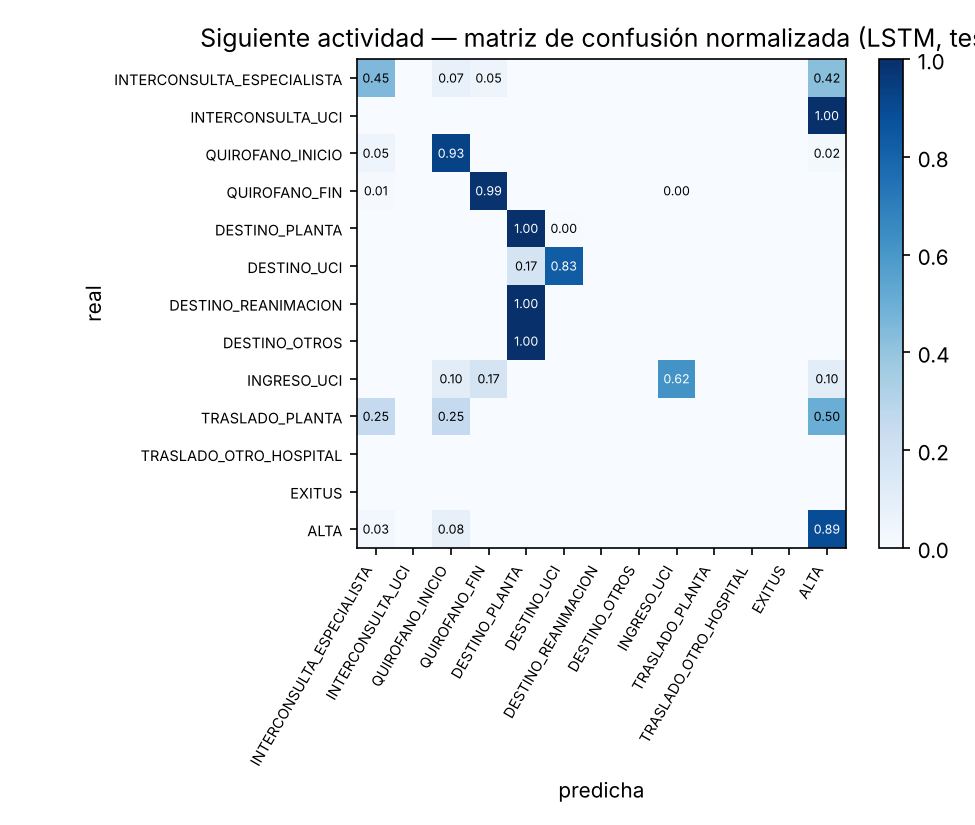
\includegraphics[width=0.75\textwidth]{nextact_confusion}
\caption{Prediction 1: row-normalized confusion matrix of the LSTM on test.}
\label{fig:confusion}
\end{figure}

The best models reach \textbf{0.91 accuracy, 4.6 points above the baseline}. The improvement comes from the fact that the destination decision, although newly added to the event log, is largely predictable: 87\% of the destinations are the ward and the \code{Gral-UCI} anesthesia anticipates \code{DESTINO\_UCI} in 88 of 122 interventions. By contrast, the \code{Gral-REA} anesthesia mostly ends in the ward (128 of 171), and therefore the post-anesthesia care unit is the exit of the operating theater that is worst predicted. The rare classes are not learned, hence the macro F1-score of 0.52--0.53; the DT with balanced weights sacrifices accuracy in favor of the rare classes. Compared with the results table of Zare et al.\ \cite{zare2025} (94\% on Helpdesk, 97\% on BPIC 2017, 60--70\% on Sepsis), the event log behaves as one of intermediate difficulty, consistent with its 3.39 bits of entropy.

\begin{table}[htbp]
\centering
\caption{Prediction 1: accuracy by prefix length on test, mean of three seeds.}
\label{tab:tarea1_k}
\small
\begin{tabular}{lrcccccc}
\toprule
$k$ & $n$ & Baseline & DT & RF & XGBoost & LSTM & Transformer \\
\midrule
1 (admission) & 295 & 0.868 & 0.834 & 0.859 & \textbf{0.875} & 0.856 & 0.858 \\
2 (in theater) & 269 & 0.922 & 0.836 & 0.908 & \textbf{0.943} & 0.939 & 0.938 \\
3 (after theater) & 265 & 0.883 & 0.616 & 0.887 & 0.923 & \textbf{0.971} & 0.970 \\
4 & 263 & 0.920 & 0.795 & \textbf{0.943} & 0.942 & 0.937 & 0.938 \\
5 & 53 & 0.415 & 0.415 & 0.679 & 0.742 & \textbf{0.805} & 0.786 \\
6 & 17 & 0.353 & 0.118 & 0.549 & \textbf{0.588} & 0.569 & 0.549 \\
\midrule
All & 1,162 & 0.867 & 0.746 & 0.883 & 0.906 & \textbf{0.913} & 0.912 \\
\bottomrule
\end{tabular}
\end{table}

Table~\ref{tab:tarea1_k} shows where the advantage of the models over the baseline comes from. At admission ($k=1$) the next event is almost always the operating theater and no model beats the trivial prediction by more than one point. The difference concentrates at the exit of the operating theater ($k=3$), where the next activity is the planned destination: the sequence models reach 0.97 against 0.88 for the baseline, because the anesthesia recorded at the start of the surgery anticipates the destination and the sequence models exploit it better than the tree-based models, which stay at 0.89--0.92. From $k=5$ onward, with 53 and 17 prefixes, the cases are the complicated episodes with consultations, ICU admissions and transfers, and the accuracy of every model except DT drops to 0.55--0.80; there the baseline collapses to 0.35--0.42, which shows that the models do learn something about the atypical trajectories even though they have few examples of them.

\section{Prediction 2: ICU Admission Without Planning Information}
\label{sec:pred2}

Table~\ref{tab:tarea2} presents the test results (860 prefixes, 70 positives, prevalence 8.1\%) and Figure~\ref{fig:tarea2_curvas} the ROC and precision--recall curves.

\begin{table}[htbp]
\centering
\caption{Prediction 2: test results, mean $\pm$ standard deviation over three seeds.}
\label{tab:tarea2}
\small
\begin{tabular}{lccccccc}
\toprule
Model & AUC-ROC & AUC-PR & F1 & Recall & Prec. & Brier & Time (s) \\
\midrule
DT & 0.754 $\pm$ 0.002 & 0.205 $\pm$ 0.004 & 0.291 & 0.34 & 0.25 & 0.165 & 0.0 \\
RF & 0.876 $\pm$ 0.002 & 0.399 $\pm$ 0.007 & 0.395 & 0.45 & 0.39 & \textbf{0.081} & 2.0 \\
XGBoost & 0.846 $\pm$ 0.005 & 0.280 $\pm$ 0.001 & 0.362 & 0.41 & 0.34 & 0.111 & 0.3 \\
LSTM & \textbf{0.886} $\pm$ 0.003 & \textbf{0.413} $\pm$ 0.014 & 0.448 & 0.51 & 0.40 & 0.161 & 22.2 \\
Transformer & \textbf{0.886} $\pm$ 0.004 & 0.411 $\pm$ 0.008 & \textbf{0.455} & 0.47 & 0.44 & 0.139 & 38.6 \\
\bottomrule
\end{tabular}
\end{table}

\begin{figure}[htbp]
\centering
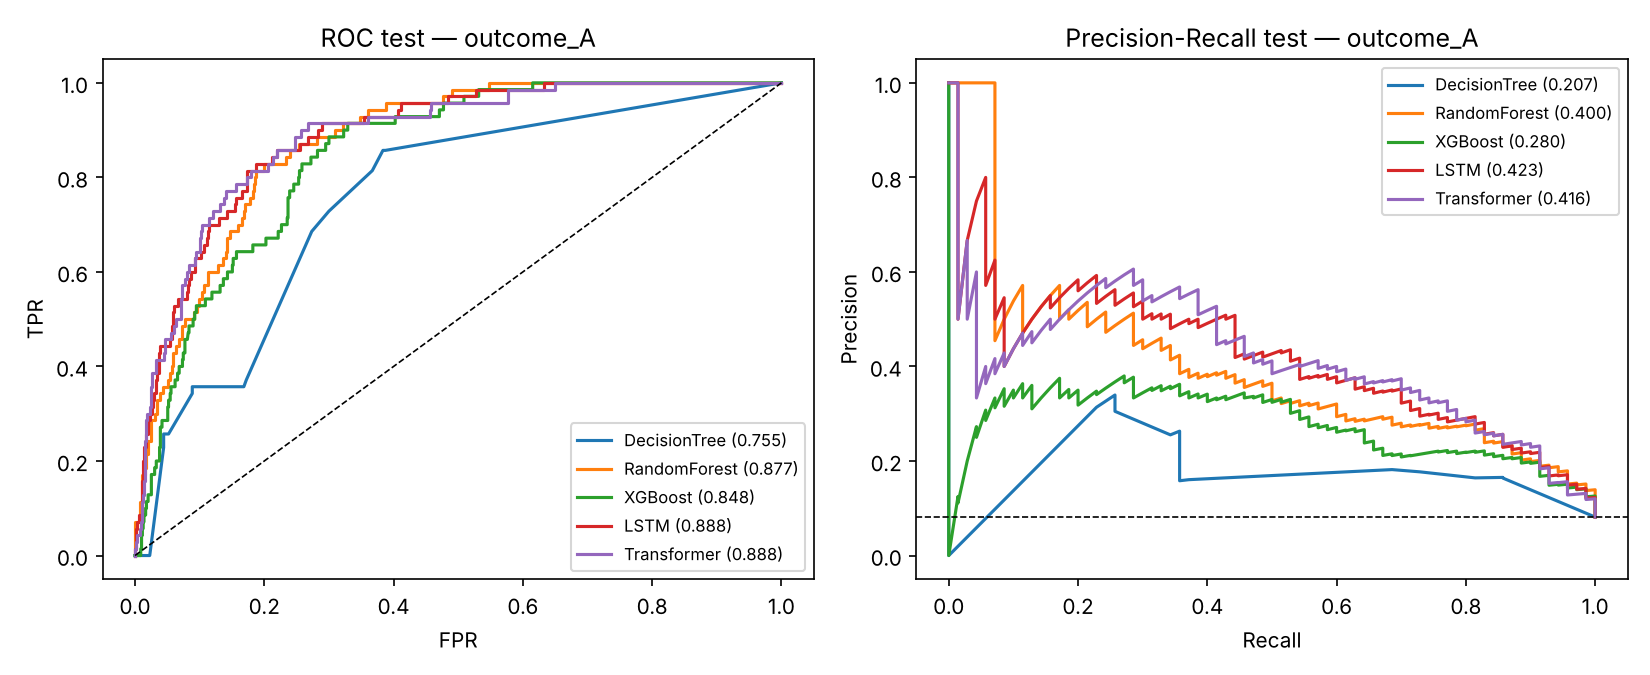
\includegraphics[width=\textwidth]{outcome_A_curvas}
\caption{Prediction 2: ROC and precision--recall curves on test.}
\label{fig:tarea2_curvas}
\end{figure}

Without the planning information, ICU admission is \textbf{predictable in a useful but not excellent way}: AUC-ROC of 0.85 to 0.89 and AUC-PR of 0.40, five times the prevalence of 8.1\%, which is the value a random classifier would obtain. LSTM and Transformer are one point above RF in AUC-ROC and on a par in AUC-PR, whereas RF is clearly the best calibrated: its Brier score of 0.081 is half that of the sequence models (0.161 for LSTM and 0.139 for Transformer), with XGBoost at 0.111 and DT at 0.165. DT and XGBoost with basic configuration are clearly behind in ranking. For reference, the same label with the planned destination in the prefix reaches an AUC-ROC of 0.969 overall and of 0.999 once the destination is in the prefix (complementary B, Section~\ref{sec:compl_b}); the gap between those values and 0.886 is exactly the planning information that variant A hides.

Table~\ref{tab:tarea2_k} and Figure~\ref{fig:tarea2_k} show how the prediction evolves with the prefix length, and Figure~\ref{fig:tarea2_imp} the variable importance. Each prefix length corresponds to a clinically meaningful moment: $k=1$ is the time of admission (295 test cases, 26 of them positive), $k=2$ is the entry into the operating theater, when the anesthesia is known (267 cases, 24 positive), and $k=3$ is the exit from the operating theater (258 cases, 19 positive). At admission, with only the patient and the service, 0.83--0.84 is already reached; in the operating theater the best models rise to 0.87--0.91; and after the operating theater to 0.92, because the anesthesia, the duration and the approach add real information about the risk. The test population shrinks with $k$ because the cases that are admitted to the ICU early, or that are discharged, stop producing prefixes.

\begin{table}[htbp]
\centering
\caption{Prediction 2: AUC-ROC per prefix length on test.}
\label{tab:tarea2_k}
\small
\begin{tabular}{lcccccc}
\toprule
$k$ & $n$ (positives) & DT & RF & XGBoost & LSTM & Transformer \\
\midrule
1 (admission) & 295 (26) & 0.723 & \textbf{0.843} & 0.799 & 0.832 & 0.825 \\
2 (in theater) & 267 (24) & 0.773 & 0.870 & 0.844 & 0.897 & \textbf{0.905} \\
3 (after theater) & 258 (19) & 0.773 & 0.921 & 0.894 & \textbf{0.924} & \textbf{0.924} \\
\bottomrule
\end{tabular}
\end{table}

\begin{figure}[htbp]
\centering
\begin{subfigure}[t]{0.56\textwidth}
\centering
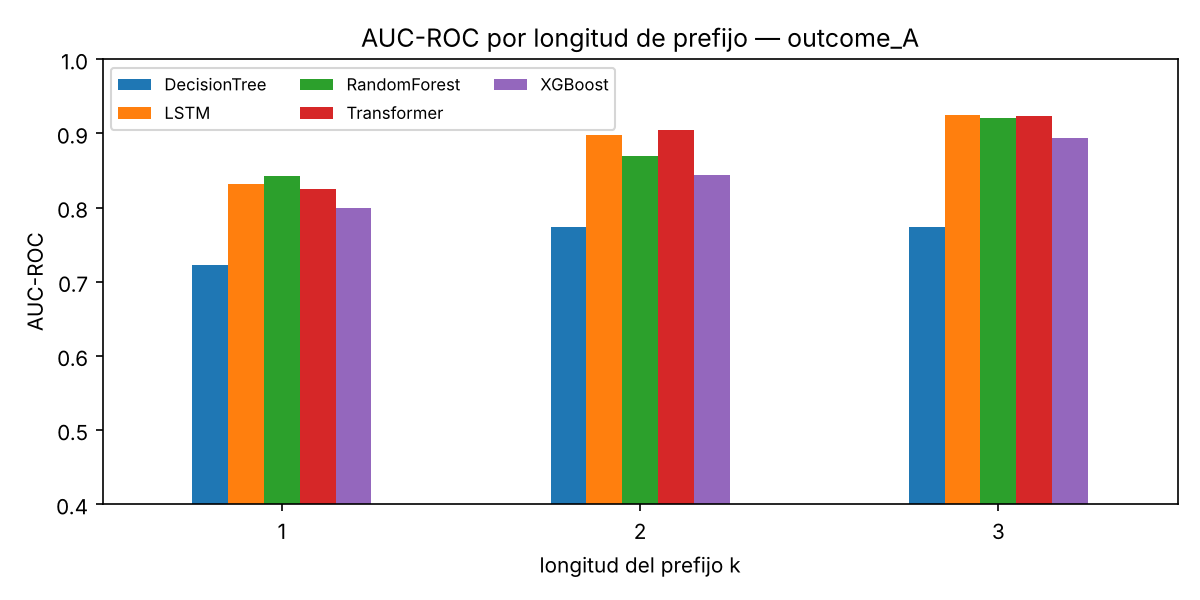
\includegraphics[width=\textwidth]{outcome_A_auc_por_prefijo}
\caption{AUC-ROC per prefix length.}
\label{fig:tarea2_k}
\end{subfigure}
\hfill
\begin{subfigure}[t]{0.42\textwidth}
\centering
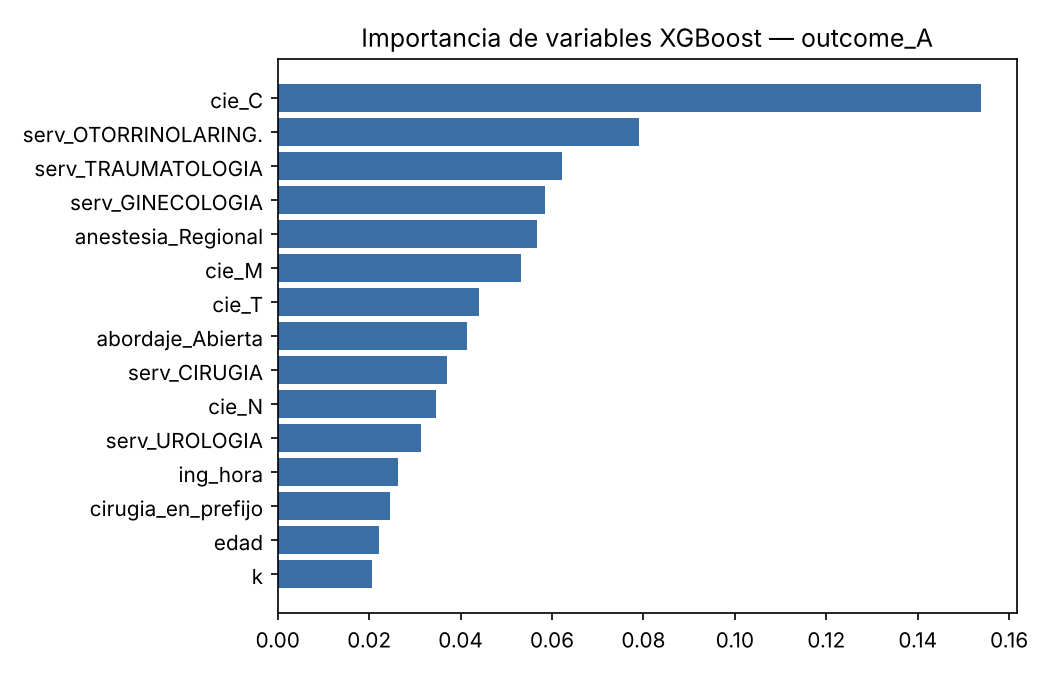
\includegraphics[width=\textwidth]{outcome_A_importancia_xgb}
\caption{Variable importance (XGBoost).}
\label{fig:tarea2_imp}
\end{subfigure}
\caption{Prediction 2: evolution with the prefix and variable importance.}
\label{fig:tarea2_evol}
\end{figure}

The most important variables (Figure~\ref{fig:tarea2_imp}) are, for RF, ICD chapter C (neoplasms, importance 0.12), age (0.12), the hour of admission (0.10), the elapsed times (0.07), the day of the week, and the orthopedics and otorhinolaryngology services as low-risk indicators. For XGBoost, the most important are chapter C again (0.15), otorhinolaryngology, orthopedics and gynecology, regional anesthesia, chapters M and T, and the open approach. The signal lies in the patient and surgery attributes, not in the order of the events, which explains why the tree-based models come so close to the networks. The results agree with those obtained on version 2 of the event log (0.85--0.88): variant A contains the same information, and therefore the new event log changes nothing when the destination is ignored.

\section{Prediction 3: Prolonged Length of Stay}

Prolonged length of stay is defined as a stay above the 90th percentile of the population, 8.74 days (148 cases). Table~\ref{tab:tarea3} and Figure~\ref{fig:tarea3_curvas} report the test results (1,160 prefixes, 137 positives, prevalence 11.8\%).

\begin{table}[htbp]
\centering
\caption{Prediction 3: test results, mean $\pm$ standard deviation over three seeds.}
\label{tab:tarea3}
\small
\begin{tabular}{lccccccc}
\toprule
Model & AUC-ROC & AUC-PR & F1 & Recall & Prec. & Brier & Time (s) \\
\midrule
DT & 0.829 $\pm$ 0.000 & 0.416 $\pm$ 0.000 & 0.569 & 0.64 & 0.51 & 0.148 & 0.0 \\
RF & 0.896 $\pm$ 0.000 & 0.475 $\pm$ 0.012 & 0.581 & 0.60 & 0.57 & \textbf{0.091} & 1.9 \\
XGBoost & 0.883 $\pm$ 0.004 & 0.478 $\pm$ 0.013 & 0.540 & 0.53 & 0.55 & 0.119 & 0.2 \\
LSTM & \textbf{0.901} $\pm$ 0.002 & \textbf{0.547} $\pm$ 0.010 & \textbf{0.606} & 0.64 & 0.58 & 0.127 & 14.3 \\
Transformer & 0.887 $\pm$ 0.002 & 0.533 $\pm$ 0.006 & 0.547 & 0.53 & 0.57 & 0.148 & 28.9 \\
\bottomrule
\end{tabular}
\end{table}

\begin{figure}[htbp]
\centering
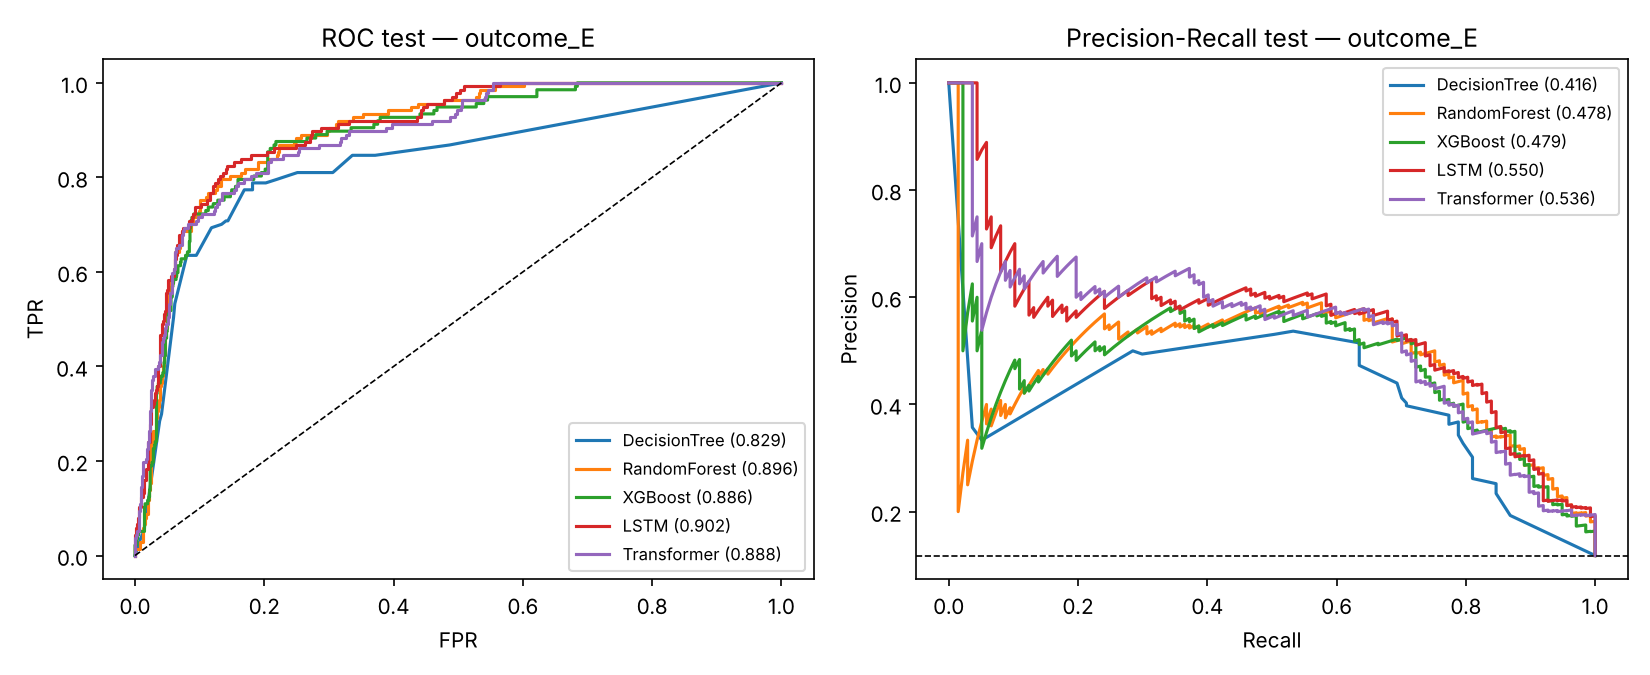
\includegraphics[width=\textwidth]{outcome_E_curvas}
\caption{Prediction 3: ROC and precision--recall curves on test.}
\label{fig:tarea3_curvas}
\end{figure}

Prolonged length of stay is the \textbf{best-predicted target}: AUC-ROC of 0.88 to 0.90 and AUC-PR of 0.47 to 0.55, four to five times the prevalence of 11.8\%, values of the order of those published in the PPM literature for this target. The pattern of Prediction~2 is repeated: LSTM wins in AUC-ROC, AUC-PR and F1-score, RF is half a point behind and is the best calibrated (Brier 0.091, against 0.119 for XGBoost, 0.127 for LSTM and 0.148 for DT and Transformer), and Transformer is slightly behind LSTM. The target depends largely on what is known at admission (the service, with general surgery as the main risk indicator, the type and duration of the surgery and the age) and on the time already elapsed, as the evolution by prefix length in Table~\ref{tab:tarea3_k} shows.

\begin{table}[htbp]
\centering
\caption{Prediction 3: AUC-ROC per prefix length on test.}
\label{tab:tarea3_k}
\begin{tabular}{lcccccc}
\toprule
$k$ & $n$ (positives) & DT & RF & XGBoost & LSTM & Transformer \\
\midrule
1 & 295 (29) & 0.762 & 0.836 & 0.817 & \textbf{0.840} & 0.819 \\
2 & 269 (28) & 0.780 & 0.879 & 0.866 & \textbf{0.899} & 0.882 \\
3 & 265 (28) & 0.840 & \textbf{0.922} & 0.906 & 0.919 & 0.913 \\
4 & 263 (27) & 0.838 & \textbf{0.920} & 0.907 & 0.918 & 0.908 \\
5 & 53 (17) & 0.785 & 0.820 & 0.817 & \textbf{0.842} & 0.840 \\
6 & 15 (8) & 0.688 & 0.589 & 0.696 & 0.732 & \textbf{0.750} \\
\bottomrule
\end{tabular}
\end{table}

By prefix length (Table~\ref{tab:tarea3_k} and Figure~\ref{fig:tarea3_k}), the starting point at admission is 0.82--0.84 and after the operating theater 0.92 is reached. From $k=5$ onward the AUC-ROC drops, but those prefixes are few (53 and 15 in test) and correspond to already complicated episodes, in which a third or a half are positive: distinguishing between patients who have already been admitted for several days is a different and harder problem. Elapsed time is the main variable (importance 0.16 in RF and 0.12 in XGBoost, Figure~\ref{fig:tarea3_imp}); in XGBoost it is followed by the general surgery service, the \code{Gral-UCI} and general anesthesia and the orthopedics service, and in RF by the hour of admission, age, surgery duration, the general surgery service and the \code{Gral-UCI} anesthesia. It is a legitimate variable, since at prediction time it is known how long the patient has been admitted, but it should be made explicit: a prefix that is already on day 7 is almost certainly positive. Run without the planning information, the prediction loses between 1.5 and 2 points of AUC-ROC (LSTM 0.885, RF 0.879): the planned destination informs about the length of stay but does not determine it, and the ranking of the models does not change.

\begin{figure}[htbp]
\centering
\begin{subfigure}[t]{0.56\textwidth}
\centering
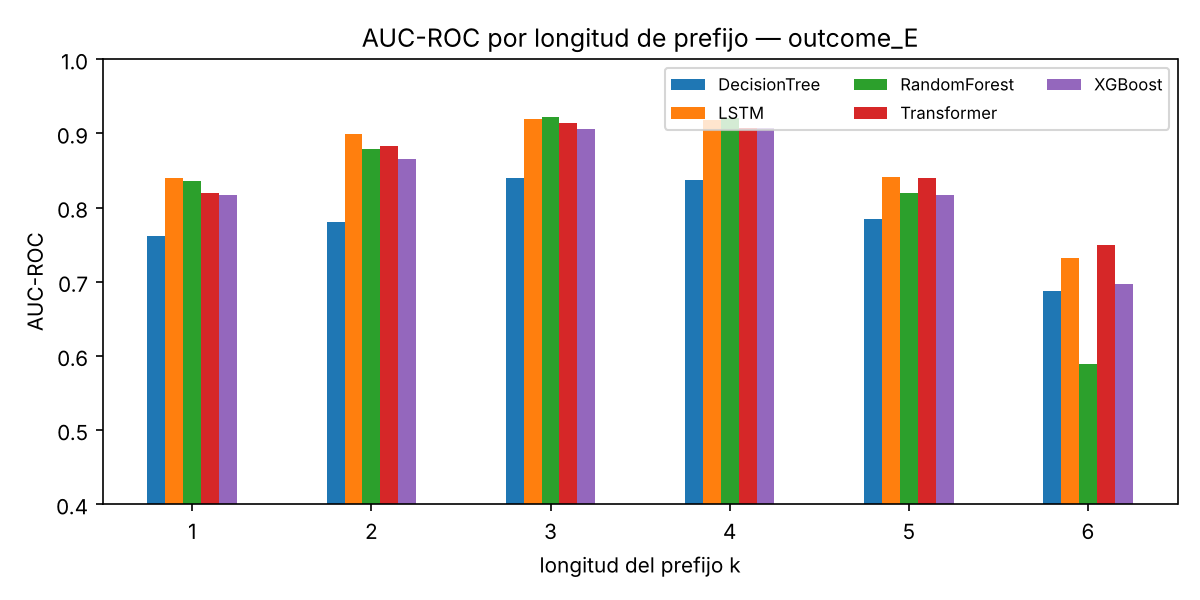
\includegraphics[width=\textwidth]{outcome_E_auc_por_prefijo}
\caption{AUC-ROC per prefix length.}
\label{fig:tarea3_k}
\end{subfigure}
\hfill
\begin{subfigure}[t]{0.42\textwidth}
\centering
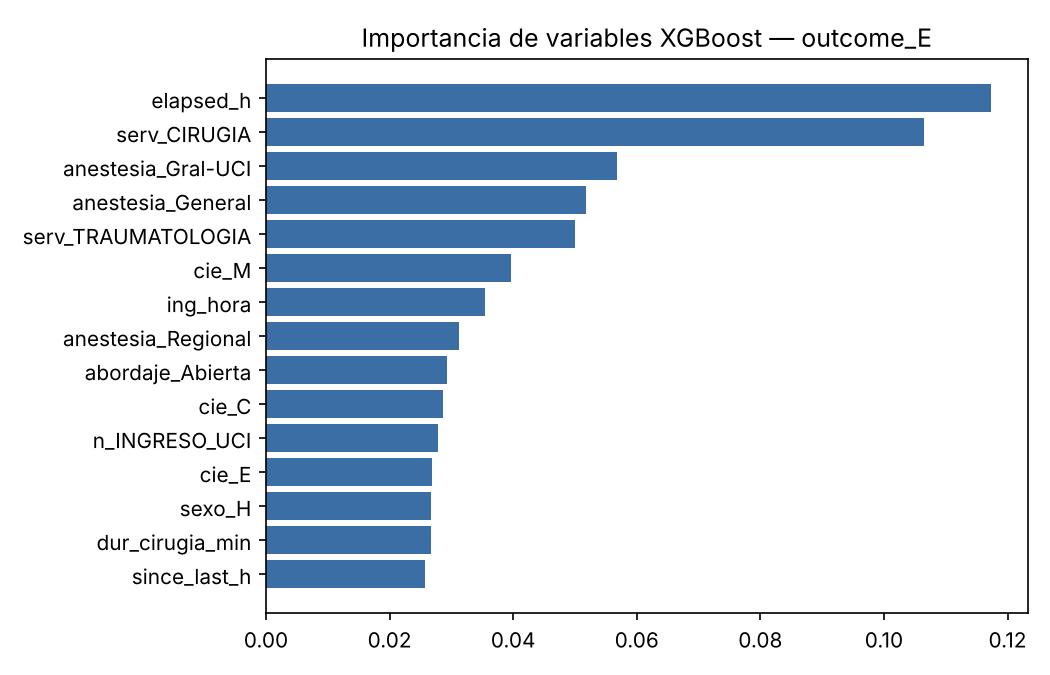
\includegraphics[width=\textwidth]{outcome_E_importancia_xgb}
\caption{Variable importance (XGBoost).}
\label{fig:tarea3_imp}
\end{subfigure}
\caption{Prediction 3: evolution with the prefix and variable importance.}
\label{fig:tarea3_evol}
\end{figure}

\section{Complementary Analyses}

The three predictions above are completed with four complementary analyses, which do not add new predictions but justify the design of Prediction~2 and measure the sensitivity of the results. The first two, B and C, are the other two ways of asking the ICU admission question introduced in Section~\ref{sec:destino_uci}: with the planning information in the prefix (B) and restricted to the unplanned admissions (C). The third, D, evaluates the broad postoperative complication label of Table~\ref{tab:etiquetas}. The fourth measures what happens when the number of coded diagnoses, excluded as leakage in Section~\ref{sec:fugas}, is included.

\subsection{ICU Admission With the Destination in the Prefix (B)}
\label{sec:compl_b}

When Prediction~2 is run with the \code{DESTINO\_*} events and the original anesthesia, AUC-ROC rises to 0.969 (RF) and 0.960 (LSTM), and AUC-PR to 0.80 (Table~\ref{tab:compl_bc}, Figure~\ref{fig:B}). By prefix length, RF goes from 0.844 at admission to 0.978 in the operating theater (with the \code{Gral-UCI} anesthesia) and to \textbf{0.999 once the destination is in the prefix}. With the destination, the prediction is trivial; before the destination, the anesthesia already reveals almost the same. That is why B is not a predictive result but the measure of how much of ICU admission is decided in advance, which is most of it, and why Prediction~2 is variant A.

\begin{table}[htbp]
\centering
\caption{Complementary B and C: AUC-ROC and AUC-PR on test (B) and out of sample with cross-validation (C, prefix at the exit of the operating theater).}
\label{tab:compl_bc}
\begin{tabular}{lcccc}
\toprule
 & \multicolumn{2}{c}{B: with destination} & \multicolumn{2}{c}{C: unplanned ICU} \\
\cmidrule(lr){2-3}\cmidrule(lr){4-5}
Model & AUC-ROC & AUC-PR & AUC-ROC & AUC-PR \\
\midrule
DT & 0.882 & 0.695 & 0.657 $\pm$ 0.053 & 0.035 \\
RF & \textbf{0.969} & \textbf{0.806} & \textbf{0.873} $\pm$ 0.021 & 0.059 \\
XGBoost & 0.936 & 0.744 & 0.635 $\pm$ 0.007 & 0.025 \\
LSTM & 0.960 & 0.800 & 0.679 $\pm$ 0.059 & 0.035 \\
Transformer & 0.956 & 0.785 & 0.715 $\pm$ 0.033 & \textbf{0.070} \\
\bottomrule
\end{tabular}
\end{table}

\begin{figure}[htbp]
\centering
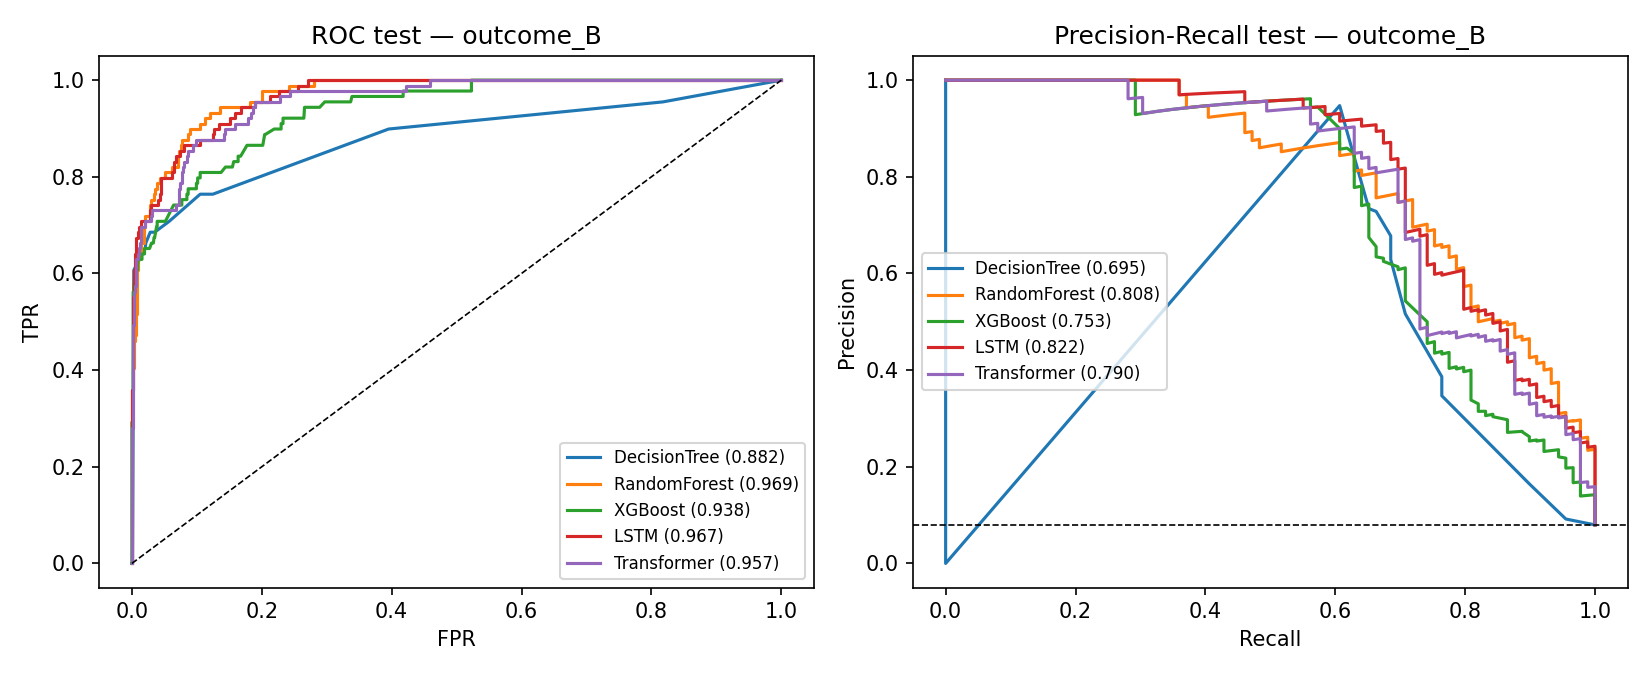
\includegraphics[width=\textwidth]{outcome_B_curvas}
\caption{Complementary B: ROC and precision--recall curves with the destination in the prefix.}
\label{fig:B}
\end{figure}

\subsection{Unplanned ICU Admission (C)}
\label{sec:compl_c}

The target is the 21 episodes that ended up in the ICU without a planned ICU destination, in the population of 1,365 cases without \code{DESTINO\_UCI}; here the planned destination is legitimate information, because no positive has it. With the temporal split the test set would contain only three positives, and therefore the evaluation uses stratified five-fold cross-validation by case with three repetitions, measuring on the prefix ending in \code{DESTINO\_*}, i.e., at the exit of the operating theater (1,220 prefixes, 11 positives, prevalence 0.9\%). RF separates the cases well (AUC-ROC 0.873, Figure~\ref{fig:C}) and assigns the ward patients who ended up in the ICU an average risk four times higher than the rest (0.099 versus 0.023). However, with that prevalence the AUC-PR is 0.06: out of every 15 or 20 alerts, one would be a real case. The deep models and XGBoost do not learn with 21 positives (0.64--0.72). It is the most clinically relevant target, but with 21 cases it allows only an exploratory analysis.

\begin{figure}[htbp]
\centering
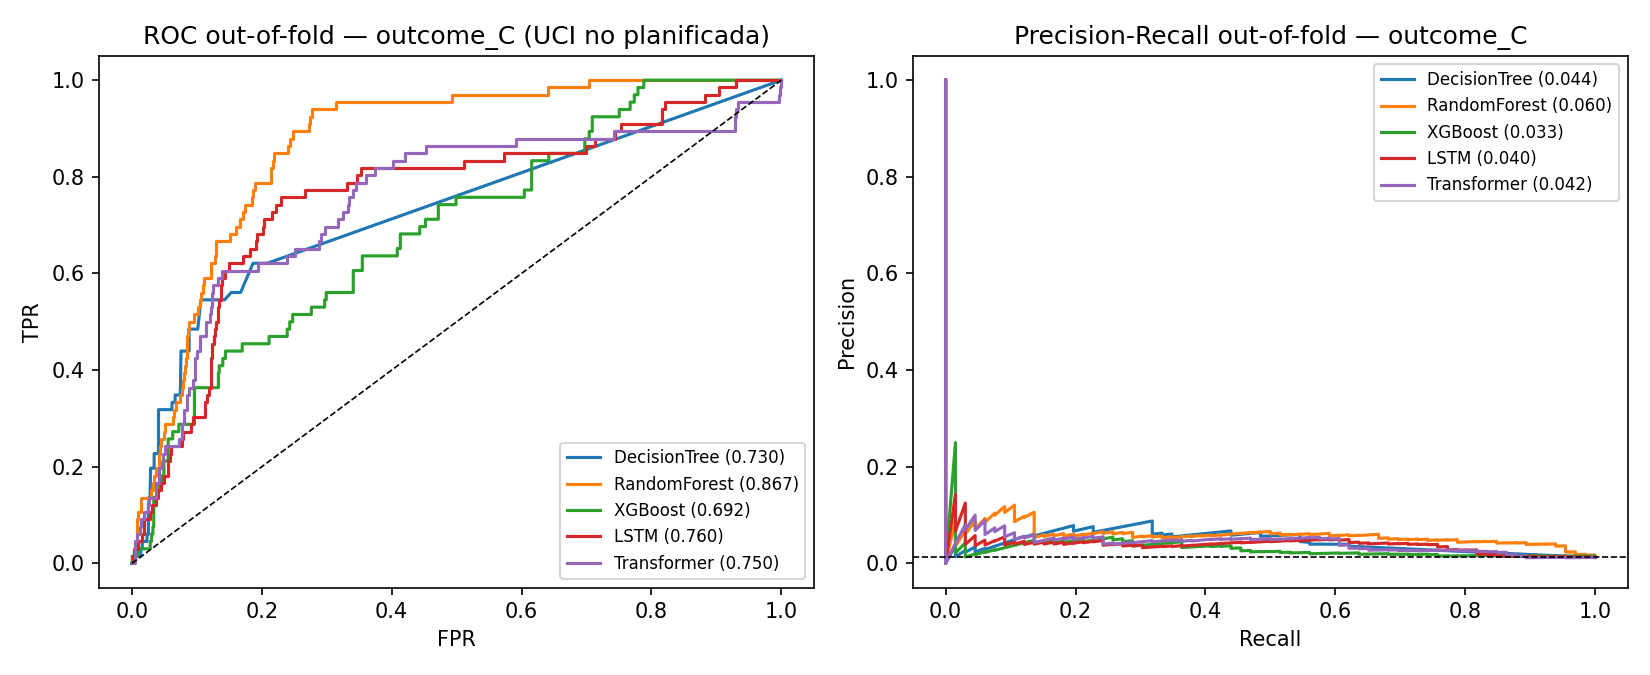
\includegraphics[width=\textwidth]{outcome_C_cv_curvas}
\caption{Complementary C: out-of-sample curves (cross-validation) for unplanned ICU admission.}
\label{fig:C}
\end{figure}

\subsection{The Broad Postoperative Complication (D)}

The postoperative complication label (240 cases: 114 postoperative ICU admissions, 165 postoperative specialist consultations, nine deaths and one transfer) was tested with the same recipe as Prediction~2. It is the hardest target (Table~\ref{tab:D}, Figure~\ref{fig:D}): AUC-ROC of 0.76 to 0.78 and AUC-PR of 0.37 to 0.42, three times the prevalence (13.2\%). It is also the only one in which the tree-based models beat the deep models: RF is the best in all metrics and the sequence models are two points below. The reason lies in the label: two thirds of the positives are postoperative consultations, a soft event that may be routine rather than complication, and 105 are planned ICU admissions (105 of the 110 cases with destination ICU; in the other five the transfer is recorded before the first surgery and does not count as postoperative). With the destination in the prefix RF rises to 0.845 / 0.636, far from the 0.999 of B: the unplanned part of the complication remains hard with or without destination. By prefix length, the signal is already present at the entry into the operating theater ($k=2$, AUC-ROC 0.81 for RF) and the postoperative events add nothing afterward, which again points to the heterogeneity of the label rather than to a lack of information in the prefix. For these reasons it is not included as a prediction of the work; if it were to be recovered, a reasonable alternative would be to define an `unplanned complication' excluding the 105 cases with \code{DESTINO\_UCI} (135 positives).

\begin{table}[htbp]
\centering
\caption{Complementary D: postoperative complication without planning, test results (835 prefixes, 110 positives).}
\label{tab:D}
\begin{tabular}{lcccc}
\toprule
Model & AUC-ROC & AUC-PR & F1 & Brier \\
\midrule
DT & 0.761 $\pm$ 0.000 & 0.313 $\pm$ 0.000 & 0.366 & 0.197 \\
RF & \textbf{0.781} $\pm$ 0.004 & \textbf{0.422} $\pm$ 0.012 & \textbf{0.444} & \textbf{0.129} \\
XGBoost & 0.775 $\pm$ 0.007 & 0.380 $\pm$ 0.015 & 0.432 & 0.162 \\
LSTM & 0.758 $\pm$ 0.001 & 0.374 $\pm$ 0.023 & 0.411 & 0.176 \\
Transformer & 0.761 $\pm$ 0.008 & 0.372 $\pm$ 0.011 & 0.410 & 0.162 \\
\bottomrule
\end{tabular}
\end{table}

\begin{figure}[htbp]
\centering
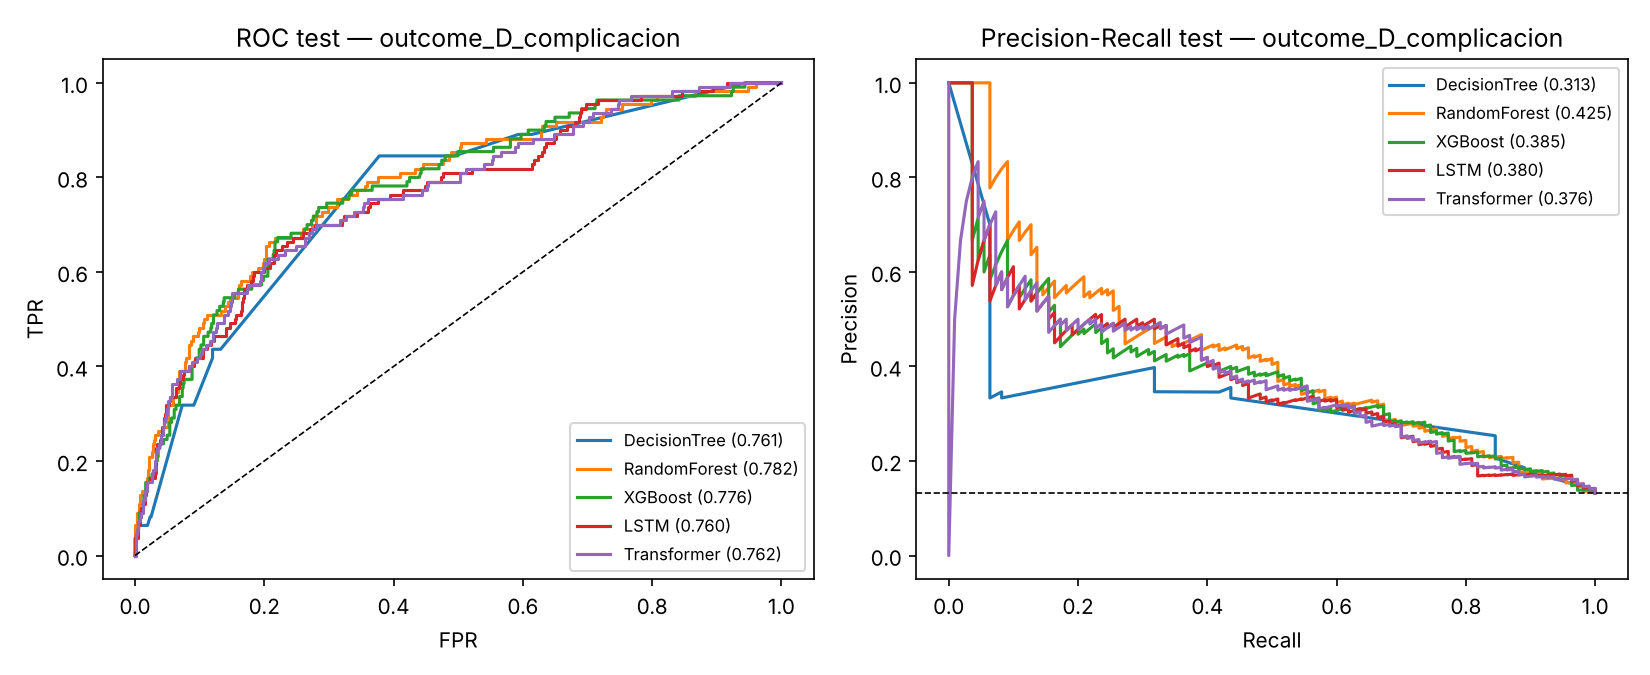
\includegraphics[width=\textwidth]{outcome_D_complicacion_curvas}
\caption{Complementary D: ROC and precision--recall curves for postoperative complication.}
\label{fig:D}
\end{figure}

\subsection{Sensitivity to the Number of Diagnoses}
\label{sec:sens_ndiag}

All the previous results exclude the \code{n\_diag} variable. Table~\ref{tab:ndiag} shows what happens when it is included. In the predictions with signal of their own the effect is mixed and small; in unplanned ICU admission, \code{n\_diag} doubles the AUC-PR and becomes the most important variable (0.21). It is the leakage symptom that was to be expected, since the complication generates diagnoses, and confirms the decision to exclude it. In the test on version 2 of the event log, the static-variable filter of LSTM and Transformer already excluded it unintentionally; in the final version the models are compared with the same information.

\begin{table}[htbp]
\centering
\caption{Sensitivity to \code{n\_diag}: AUC-ROC / AUC-PR with and without the variable.}
\label{tab:ndiag}
\begin{tabular}{lcc}
\toprule
Experiment & Without \code{n\_diag} (main) & With \code{n\_diag} \\
\midrule
Prediction~2 $\cdot$ RF & 0.876 / 0.399 & 0.853 / 0.451 \\
Prediction~2 $\cdot$ XGBoost & 0.846 / 0.280 & 0.755 / 0.353 \\
B $\cdot$ RF & 0.969 / 0.806 & 0.954 / 0.760 \\
C $\cdot$ RF, exit of the operating theater & 0.873 / 0.059 & 0.928 / 0.116 \\
\bottomrule
\end{tabular}
\end{table}

\section{Synthesis and Comparison With the Entropy-Driven Next Activity Prediction Approach}

\subsection{The Three Targets Side by Side}

Figure~\ref{fig:sintesis} shows the main metric of each prediction by model, and Table~\ref{tab:sintesis} gathers the main results of the three outcome-based targets (Predictions~2 and 3 and the complementary analysis D). Together they allow three observations.

\begin{figure}[htbp]
\centering
\begin{tikzpicture}
\begin{axis}[
  ybar, width=0.95\textwidth, height=7.6cm, bar width=11pt,
  ymin=0.70, ymax=0.98, xmin=-0.6, xmax=4.6,
  ylabel={Main metric on test (mean of three seeds)}, ylabel style={font=\small},
  xtick={0,1,2,3,4}, xticklabels={DT, RF, XGBoost, LSTM, Transformer},
  tick label style={font=\footnotesize},
  nodes near coords, nodes near coords style={font=\tiny, rotate=90, anchor=west, /pgf/number format/fixed, /pgf/number format/precision=3, /pgf/number format/fixed zerofill},
  axis x line*=bottom, axis y line*=left,
  legend style={at={(0.5,-0.14)}, anchor=north, legend columns=3, font=\footnotesize, draw=black!30}]
\addplot[fill=green!55!black, draw=green!55!black] coordinates {(0,0.746) (1,0.883) (2,0.906) (3,0.913) (4,0.912)};
\addplot[fill=blue!60, draw=blue!60] coordinates {(0,0.754) (1,0.876) (2,0.846) (3,0.886) (4,0.886)};
\addplot[fill=orange!80, draw=orange!80] coordinates {(0,0.829) (1,0.896) (2,0.883) (3,0.901) (4,0.887)};
\legend{Prediction~1: accuracy, Prediction~2: AUC-ROC, Prediction~3: AUC-ROC}
\draw[green!55!black, dashed] (axis cs:-0.6,0.867) -- (axis cs:4.6,0.867);
\node[font=\tiny, green!45!black, anchor=north west] at (axis cs:-0.58,0.866) {Prediction~1 baseline 0.867};
\end{axis}
\end{tikzpicture}
\caption{Main metric of each prediction on test by model: accuracy for Prediction 1 and AUC-ROC for Predictions 2 and 3, mean of three seeds. The dashed line is the most-frequent-transition baseline of Prediction 1.}
\label{fig:sintesis}
\end{figure}

\begin{table}[htbp]
\centering
\caption{Synthesis: AUC-ROC / AUC-PR on test for the three outcome targets.}
\label{tab:sintesis}
\small
\begin{tabular}{lccc}
\toprule
Model & Prediction~2 ICU & Prediction~3 Stay & D Complication \\
 & (8.1\%) & (11.8\%) & (13.2\%) \\
\midrule
DT & 0.754 / 0.205 & 0.829 / 0.416 & 0.761 / 0.313 \\
RF & 0.876 / 0.399 & 0.896 / 0.475 & \textbf{0.781 / 0.422} \\
XGBoost & 0.846 / 0.280 & 0.883 / 0.478 & 0.775 / 0.380 \\
LSTM & \textbf{0.886 / 0.413} & \textbf{0.901 / 0.547} & 0.758 / 0.374 \\
Transformer & \textbf{0.886 / 0.411} & 0.887 / 0.533 & 0.761 / 0.372 \\
\midrule
AUC-PR / prevalence & $\times$5.1 & $\times$4.6 & $\times$3.2 \\
Minimum Brier & 0.081 (RF) & 0.091 (RF) & 0.129 (RF) \\
\bottomrule
\end{tabular}
\end{table}

First, the order of difficulty of the targets is length of stay $<$ ICU admission $<$ complication. The length of stay depends on what is known at admission. ICU admission depends on it only partly, and what is missing is revealed by the surgery. The broad complication includes events that depend on the evolution and on the practice of each service. Second, the winner depends on the signal: with enough signal (Predictions~1, 2 and 3) the sequence models win in ranking, but by a small margin over RF: 3.0 points of accuracy in Prediction~1, 1.0 point of AUC-ROC in Prediction~2 and 0.5 in Prediction~3. With weak signal or few positives (complementary analyses D and C) RF wins. Transformer and LSTM are indistinguishable in Prediction~1 (0.912 versus 0.913) and in Prediction~2 (0.886 for both), and LSTM is 1.4 points ahead in Prediction~3. Third, RF is the best calibrated in the three targets (Brier 0.08--0.13 versus 0.13--0.18 for the deep models), the one that suffers least when the target gets harder and the cheapest (2 s versus 13--40 s). Transformer does not outperform LSTM in any case with traces of one to six events.

\subsection{Comparison with the Protocol of the Entropy-Driven Next Activity Prediction Approach}

Table~\ref{tab:zare_vs} contrasts the experimental protocol of this work with that of the reference paper, based on the parameters it publishes (its Section 4.1 and its Tables 2 and 3).

\begin{table}[htbp]
\centering
\caption{Experimental protocol of the Entropy-Driven Next Activity Prediction Approach versus that of this work.}
\label{tab:zare_vs}
\small
\begin{tabular}{L{2.4cm}L{5.4cm}L{5.4cm}}
\toprule
Parameter & Entropy-Driven Next Activity Prediction Approach & This work \\
\midrule
Predictions & Next-activity prediction only & Next-activity prediction (Prediction~1) and two outcome-based predictions (Predictions~2 and 3) \\
Event logs & Six public ones, from 781 to 150,370 cases & One built for this work, 1,475 cases \\
Prefixes & Complete history padded to the longest trace & $k$-prefixes from 1 to 6; with a median of five they cover almost the whole history \\
Split & 80 / 20 training--validation, `separate' test set without details & Temporal by case, 64 / 16 / 20 \\
Repetitions & No seeds or standard deviations reported & Three seeds, mean $\pm$ standard deviation \\
Imbalance & Subsampling, only for the Transformer on Road Traffic Fine & Class weights in the models \\
Metrics & Accuracy and entropy of the confusion matrix & AUC-ROC, AUC-PR, F1-score, Brier, AUC per prefix; accuracy and macro F1-score \\
Recurrent model & CNN-BiLSTM: convolutions 64/128/256, BiLSTM 400, 300 epochs, batch 32 & LSTM 64 units, embedding 16, up to 80 epochs, batch 64 \\
Transformer & DAW-Transformer: embedding 256, 8 heads, FFN 256, batch 2, 50 epochs & $d=32$, 4 heads, 2 layers, FFN 64, dropout 0.1 \\
Tree-based models & Hyperparameters not published & DT depth 6; RF 300 trees; XGBoost 400 trees with early stopping \\
\bottomrule
\end{tabular}
\end{table}

Three differences deserve comment. The deep models of this work are much smaller than those of the paper ($d=32$ versus 256; 64 units versus 400). This is consistent with the size of the event log (four to six thousand prefixes versus tens or hundreds of thousands of events), but it leaves open the question of whether a larger model would change the conclusion. The paper uses the complete history of the case and criticizes fixed-length windows; in this event log, with a median of five events, six prefixes are practically the whole history, and therefore the difference is only nominal. Moreover, the protocol of this work is stricter in three respects (temporal split, repetition with seeds and imbalance-sensitive metrics), which makes it possible to trust that differences of half a point between models are not noise.

The conclusion, on the other hand, is shared: on a medium-entropy event log, the advantage of the deep models over the classical ensemble is small. What the paper shows with six public event logs on next-activity prediction is reproduced here with a clinical event log built for this work and on three predictions.

\chapter{Conclusions}
\label{cap:conclusiones}

This chapter presents the conclusions drawn during the work and after its completion: the personal ones, those derived from the study in relation to the objectives set, and the limitations and lines of future work.

\section{Personal Conclusions}

This work has been the point where the subjects of the master's degree stopped being separate pieces and became one method. The subject \emph{Process Mining} (SJK013) gave me the vocabulary and the tools of the first half of the work: the event log, the discovery algorithms, conformance checking and the way of reading a process from its data. \emph{Machine Learning} (SJK003) gave me the models and, above all, the discipline of the evaluation protocol: a temporal split, class imbalance, several seeds and metrics that answer the clinical question and not only the numerical one. \emph{Big Data Analytics} (SJK006) gave me the habits of working with data in Python, from the loading and cleaning of tables to the reproducible organization of scripts, results and figures. Without the three subjects this work would not have been possible in the time available.

The main lesson has been that, with real clinical data, most of the effort goes to the data and not to the models. The database had to be understood table by table, the scope had to be reduced twice before the event log was useful, and every activity and attribute had to be justified. The most valuable finding of the work, that the postoperative destination is planning and not prediction, did not come from a model but from reading the conformance results and the attributes by phase. I have learned to distrust a very good result and to look for the leak before celebrating it. My professional background in information security and auditing helped me here, because the questions are the same: where does this information come from, who recorded it and when.

I have also learned the value of defining the scope early and of documenting each phase as it closes. The intermediate reports of the event log, the discovery and the experiments were what made it possible to write this report in a short time and to answer the questions of the supervisors with evidence. Finally, the work has shown me that process mining and predictive process monitoring are a realistic way of bringing artificial intelligence to a hospital: they start from the data the hospital already records, they produce models that the clinical staff can read, and they make explicit what the organization plans and what it does not foresee. I would like to continue in this line, with a larger event log and in contact with the clinical team of the project.

\section{Conclusions Derived From the Study}

The development of the work has made it possible to fulfill the objectives set in the proposal, with the scope narrowed to the elective surgical admission process. The methodology followed (iterative construction of the event log, validation with several PM tools, incremental experimental design and evaluation with a strict protocol) has produced consistent and reproducible results. In relation to the objectives of Section~\ref{sec:objetivos}, numbered as there, the following conclusions stand out:

\begin{itemize}[leftmargin=*]
  \item \textbf{Objective 1. Transformation of the database into an event log.} An event log of 1,475 episodes, 7,780 events and 14 activities was built from four event tables of \code{ftr\_cige\_v01}, with a design decision that proved decisive: separating the planned postoperative destination (a decision recorded in the operating theater) from the actual transfer (a movement with its own time). The four PM tools read the event log identically.
  \item \textbf{Objective 2. Analysis of the event log through discovery and conformance.} The Heuristics Miner is the best discovered model (fitness 0.97--0.98 in ProM and PM4Py, and precision 0.92 in PM4Py). The reference BPMN model, with the ICU bed reservation read as the postoperative destination, explains 81\% of the traces in two independent implementations (Celonis and PM4Py) and flags the unplanned ICU admission as a deviation from the planned destination. The central finding is that \textbf{the postoperative destination is planning, not prediction}: \code{DESTINO\_UCI} implies \code{INGRESO\_UCI} in all 110 cases.
  \item \textbf{Objectives 3 and 4. State-of-the-art study and algorithm selection.} The Entropy-Driven Next Activity Prediction Approach \cite{zare2025} (five algorithms, process entropy as framework) and the evaluation protocol of Teinemaa et al.\ for the outcome-based predictions were adopted. The entropy of the event log, 3.39 bits, places it in the medium band of the paper, for which the paper predicts that interpretable models perform close to deep ones.
  \item \textbf{Objectives 5 and 7. Implementation and evaluation of the algorithms.} The three predictions run in a single reproducible run of 551 s on CPU. The next activity is predicted with an accuracy of 0.91, 4.6 points above the baseline; ICU admission without planning information is anticipated with an AUC-ROC of 0.89 (0.84 already at admission, 0.92 after the operating theater); and prolonged length of stay with 0.90 and an AUC-PR of 0.55. Unplanned ICU admission, the most clinically relevant target, shows signal (RF 0.87 at the exit of the operating theater) but with 21 cases it allows only an exploratory analysis.
  \item \textbf{Objectives 6 and 8. Comparison of the predictive approaches.} The sequence models (LSTM and Transformer) win in ranking when there is enough signal, but by only 0.5 to 1 point of AUC-ROC over RF, which is the most robust model, the best calibrated in all the targets and the one that wins when the signal is scarce. Transformer does not outperform LSTM with traces of one to six events. The predictive signal lies in the patient and surgery attributes rather than in the sequence of events. This conclusion agrees with that of the Entropy-Driven Next Activity Prediction Approach \cite{zare2025} for medium-entropy event logs and is reproduced here with a clinical event log built for this work and on three predictions.
\end{itemize}

Another conclusion of the work is methodological: a substantial part of the effort did not consist in training models, but in identifying which information is legitimate at each prediction point. Variant B (AUC-ROC 0.999 once the destination is in the prefix) and the sensitivity to the number of diagnoses (which doubles the apparent performance on the scarcest target) show that, in real clinical data, an excellent result is frequently a symptom of leakage and not of predictive ability. Conformance analysis and the study of the attributes by phase were the tools that made it possible to detect it.

\section{Limitations and Future Work}

The work has limitations that must be taken into account:

\begin{itemize}[leftmargin=*]
  \item The event log has 1,475 episodes and the test set 295; the variability of the metrics across seeds is high and the targets with fewer than 30 positives cannot be evaluated with a temporal split.
  \item The five algorithms were run with basic configuration, without hyperparameter tuning; XGBoost and the deep models would probably improve with it.
  \item The deep models are much smaller than those of Zare et al.\ \cite{zare2025} ($d = 32$ versus 256), in accordance with the size of the event log, but it has not been checked whether a larger model would change the conclusion.
  \item The ICD chapter of the main diagnosis comes from the coding at discharge and is kept with reservations; the alternative would be to code the admission diagnosis, which is free text.
  \item The split is by case and not by patient (1,308 patients for 1,475 episodes), and therefore a patient may appear in both training and test.
  \item In prolonged length of stay, elapsed time dominates the prediction; evaluation at a fixed point of the process, such as the exit of the operating theater, could be considered.
  \item The data come from a single hospital and a single period, which limits generalization.
\end{itemize}

From these limitations, the following lines of future work are proposed, in order of priority:

\begin{itemize}[leftmargin=*]
  \item Hyperparameter tuning with temporal cross-validation in Predictions~2 and 3, and calibration of the deep models.
  \item Explainability of RF and XGBoost through SHAP values, to contrast with clinical judgment which variables support each prediction.
  \item Definition of an `unplanned complication' that excludes the planned ICU admissions (135 positives), as an intermediate target between unplanned ICU admission (21) and the broad complication (240).
  \item Extension of the population to all surgical admissions, not only elective ones, to provide more cases for the unplanned ICU admission target; this requires reopening the agreed scope.
  \item Testing of the process-model-based approaches (annotated transition systems), considered in the proposal and not addressed, to complete the comparison between the two PPM families.
  \item Development of a decision-support tool based on the Prediction~2 model, which presents the risk of ICU admission at admission and after the operating theater.
\end{itemize}

In short, the work constitutes a first step in the application of PPM to a real surgical process in an FTR context, and establishes an event log, a validated reference model and a reproducible experimental pipeline on which further research can be built.


% =====================================================================
\backmatter
% Estilo IEEE numérico por orden de aparición (IEEEtran.bst está en Overleaf)
\renewcommand{\bibname}{References}
\bibliographystyle{IEEEtran}
\bibliography{bibliografia}

\end{document}
